\documentclass[12pt,a4paper]{extreport}
\usepackage[utf8]{inputenc}
%\usepackage[T5]{fontenc}
\usepackage[utf8]{vietnam}
%\usepackage{times}
\usepackage{enumerate}
\usepackage{enumitem}
\usepackage{multicol}
\usepackage{listings}
\usepackage[a4paper, top=3.5cm,bottom=3cm,left=3.5cm,right=2cm]{geometry}
\usepackage{verbatim}
\usepackage{graphicx}
\usepackage{url}
\usepackage{fancyhdr}
\usepackage{fancybox,framed}
\linespread{1.3}
\usepackage{lastpage}
\usepackage{floatrow}
\usepackage{floatrow}
\usepackage{array}
\usepackage{longtable}

\pagenumbering{arabic}
%\pagestyle{fancy}
\newfloatcommand{capbtabbox}{table}[][\FBwidth]
\usepackage{caption}
%\captionsetup[figure]{font=normalsize}
\usepackage{blindtext}
\usepackage{titlesec}
\usepackage[nottoc]{tocbibind}
\usepackage{bookmark}
%\usepackage[backend=bibtex,style=numeric,defernumbers=true,sorting=none]{biblatex}
% \usepackage[backend=biber]{biblatex}
%\bibliographystyle{plain}
%\bibliography{References/references.bib}

% ******************************************************************************
%\setlength{\topmargin}{-0.5cm} % Lề trên
%\setlength{\oddsidemargin}{-0.5cm} % Lề trái
%\setlength{\evensidemargin}{-0.5cm} % Lề phải
\setlength{\textwidth}{15.5cm} % Chiều rộng văn bản
\setlength{\textheight}{24cm} % Chiều cao văn bản
\setlength{\footskip}{1cm} % Khoảng cách giữa nội dung và số trang

% For line spacing 1.5
%\usepackage{setspace}
%\renewcommand{\baselinestretch}{1.5}

% ******************************************************************************
\usepackage{hyperref}
% \usepackage{hyperref}

% Cấu hình cho \paragraph để nó xuống hàng sau tiêu đề
\titleformat{\paragraph}[block]
{\normalfont\normalsize\bfseries}{\theparagraph}{1em}{}

\titlespacing*{\paragraph}
{0pt}{3.25ex plus 1ex minus .2ex}{1.5ex plus .2ex}

\setcounter{secnumdepth}{4}
\setcounter{tocdepth}{4}

\usepackage{array} % Gói cần thiết cho kiểu cột m{}

\titleformat*{\section}{\LARGE\bfseries}
\titleformat*{\subsection}{\Large\bfseries}
\titleformat*{\subsubsection}{\large\bfseries}


\usepackage{mdframed}

\usepackage{alltt}
\usepackage{color}
\usepackage{tocloft}

\usepackage{tikz}
\usetikzlibrary{calc}
\newcommand\HRule{\rule{\textwidth}{1pt}}
\fancyfoot[C]{\thepage}

% Math
\usepackage{amsfonts}

\usepackage[numbers]{natbib}

%\newcommand{\tenSV}{Hoàng~Minh~Thanh} % Dấu ~ là khoảng trắng không được tách (các chữ nối với nhau bằng dấu ~ sẽ nằm cùng 1 dòng
%\newcommand{\mssv}{21C11029}
%\newcommand{\tenKL}{OPENHUMAN: HỆ THỐNG} % Chú ý dấu ~ trong tên khóa luận
\newcommand{\tenSV}{Phan~Minh~Tâm~-~Hoàng~Minh~Thanh} % Dấu ~ là khoảng trắng không được tách (các chữ nối với nhau bằng dấu ~ sẽ nằm cùng 1 dòng
\newcommand{\mssv}{18424059-18424062}
\newcommand{\tenKL}{ĐỰ~ĐOÁN~LIÊN~KẾT~TRONG~ĐỒ~THỊ~TRI~THỨC} % Chú ý dấu ~ trong tên khóa luận
\newcommand{\tenGVHD}{ThS.~Lê~Ngọc~Thành}
\newcommand{\tenBM}{BM. Khoa~Học~Máy~Tính}

\usepackage{amsmath}
\usepackage{amssymb}
\usepackage{stmaryrd}

\usepackage[font=small,labelfont=bf]{subcaption}
\usepackage{listings}
\usepackage{color}

\usepackage{tocloft}
\usepackage{tabularx}
\usepackage{booktabs}
\usepackage{multirow}

\usepackage{tocloft}
\usepackage{tabularx}
\usepackage{booktabs}


% Chèn và định dạng mã giả
\usepackage{algorithm}
% \usepackage[ruled,vlined,linesnumbered]{algorithm2e}
\usepackage[noend]{algpseudocode}
\makeatletter
\def\BState{\State\hskip-\ALG@thistlm}
\makeatother


\usepackage{float}



\usepackage{cleveref}


% Vẽ hình
\usetikzlibrary{arrows,shapes,positioning, decorations, babel, quotes}
\usepackage[babel,german=quotes]{csquotes}

% Coordinate
\usepackage{pgfplots, pgfplotstable}

\usepackage{ltablex}
% Redefine \tiny
\renewcommand{\tiny}{\fontsize{6.01}{7.21}\selectfont}    % MS Word 6pt ≈ LaTeX 6.01pt

% Redefine \scriptsize
\renewcommand{\scriptsize}{\fontsize{7.01}{8.41}\selectfont}  % MS Word 7pt ≈ LaTeX 7.01pt

% Redefine \footnotesize
\renewcommand{\footnotesize}{\fontsize{8.03}{9.63}\selectfont} % MS Word 8pt ≈ LaTeX 8.03pt

% Redefine \small
\renewcommand{\small}{\fontsize{12.03}{14.43}\selectfont}  % MS Word 12pt ≈ LaTeX 12.03pt

% Redefine \normalsize
\renewcommand{\normalsize}{\fontsize{13.04}{15.65}\selectfont} % MS Word 13pt ≈ LaTeX 13.04pt

% Redefine \large
\renewcommand{\large}{\fontsize{14.08}{16.90}\selectfont}  % MS Word 14pt ≈ LaTeX 14.08pt

% Redefine \Large
\renewcommand{\Large}{\fontsize{16.16}{19.26}\selectfont}  % MS Word 16pt ≈ LaTeX 16.16pt

% Redefine \LARGE
\renewcommand{\LARGE}{\fontsize{18.19}{21.83}\selectfont}  % MS Word 18pt ≈ LaTeX 18.19pt

% Redefine \huge
\renewcommand{\huge}{\fontsize{20.22}{24.26}\selectfont}   % MS Word 20pt ≈ LaTeX 20.22pt

% Redefine \Huge
\renewcommand{\Huge}{\fontsize{24.27}{29.12}\selectfont}   % MS Word 24pt ≈ LaTeX 24.27pt




% \titleformat{\section}[block]{\normalfont\Large\bfseries}{\thesection}{1em}{}

% \titleformat{\chapter}[display]
%   {\normalfont\LARGE\bfseries}   % Font size and weight for chapter title
%   {\thechapter}                  % Chapter number formatting
%   {1em}                          % Space between number and title
%   {}

% \makeatletter
% \def\@makechapterhead#1{
%   \vspace*{50pt}  % Vertical space before the chapter title
%   {\normalfont\Huge\bfseries\MakeUppercase{#1}}  % Font size and uppercase
%   \par\nobreak
%   \vskip 40pt
% }
% \makeatother


% \makeatletter
% \def\@makechapterhead#1{
%   \vspace*{50pt}  % Vertical space before the chapter title
%   {\normalfont\Huge\bfseries \MakeUppercase{Chapter \thechapter: #1}}  % "Chapter" text and uppercase title
%   \par\nobreak
%   \vskip 40pt
% }
% \makeatother

%********************* Custom *********************

% \Huge
% Customize chapter title (equivalent to Word styles)
\titleformat{\chapter} % Adjust the chapter heading
  {\LARGE\bfseries}     % Font size: Huge (24.27pt), bold
  {\chaptername\ \MakeUppercase\thechapter.}       % Chapter number with a period
  {20pt}               % Space between the number and title
  {\MakeUppercase}     % Title format

% Customize section title (equivalent to Word styles)
\titleformat{\section} % Adjust the section heading
  {\Large\bfseries}    % Font size: LARGE (18.19pt), bold
  {\thesection}        % Section numbering
  {15pt}               % Space between the number and title
  {\LARGE\bfseries}    % Title format

% Customize subsection title
\titleformat{\subsection} % Adjust the subsection heading
  {\large\bfseries}      % Font size: Large (16.16pt), bold
  {\thesubsection}       % Subsection numbering
  {10pt}                 % Space between the number and title
  {\Large\bfseries}      % Title format

% Customize subsubsection title
\titleformat{\subsubsection} % Adjust the subsubsection heading
{\normalsize\bfseries}      % Font size: Large (16.16pt), bold
{\thesubsubsection}       % Subsection numbering
{10pt}                 % Space between the number and title
{\normalsize\bfseries}      % Title format

%********************* Custom *********************

\definecolor{customlinkcolor}{HTML}{0064E0}
\definecolor{customcitecolor}{HTML}{00AF19}
\definecolor{custompinkcolor}{HTML}{AF00E6}


% custom color
\definecolor{awesome}{rgb}{1.0, 0.13, 0.32}
\definecolor{azure}{rgb}{0.0, 0.5, 1.0}
\definecolor{amber}{rgb}{1.0, 0.75, 0.0}
\definecolor{deepmagenta}{rgb}{0.8, 0.0, 0.8}
\definecolor{darkpastelgreen}{rgb}{0.01, 0.75, 0.24}
\definecolor{deepskyblue}{rgb}{0.0, 0.75, 1.0}
\definecolor{deepcarminepink}{rgb}{0.94, 0.19, 0.22}
\definecolor{gray}{rgb}{0.5, 0.5, 0.5}


\definecolor{codegreen}{rgb}{0,0.6,0}
\definecolor{codegray}{rgb}{0.5,0.5,0.5}
\definecolor{codepurple}{rgb}{0.58,0,0.82}
\definecolor{backcolour}{rgb}{0.95,0.95,0.92}
\lstdefinestyle{mystyle}{
    backgroundcolor=\color{backcolour},   
    commentstyle=\color{codegreen},
    keywordstyle=\color{magenta},
    numberstyle=\tiny\color{codegray},
    stringstyle=\color{codepurple},
    basicstyle=\footnotesize,
    breakatwhitespace=false,         
    breaklines=true,                 
    captionpos=b,                    
    keepspaces=true,                 
    numbers=left,                    
    numbersep=5pt,                  
    showspaces=false,                
    showstringspaces=false,
    showtabs=false,                  
    tabsize=2
}
\lstset{style=mystyle}


\hypersetup{
	colorlinks=true,
	linkcolor=customlinkcolor,
	citecolor=customcitecolor,
	filecolor=magenta,
	urlcolor=custompinkcolor,
	citebordercolor=red,
	breaklinks=true,
	bookmarksopen=true,
	frenchlinks=true,
	linkbordercolor={0 0 1},
	menubordercolor={0 0 1},
	plainpages=false,
	urlbordercolor={0 0 1},
	pdftitle={Link Prediction In Knowledge Graphs Using Graph Collaborative Attention Network},
	pdfauthor={Hoang Minh Thanh - Phan Minh Tam},
	pdfpagemode=FullScreen,
	pdfborder={0 0 0}
}


% Abstract
\usepackage{changepage}

\newcommand{\der}[2]{\frac{d#1}{d#2}}
\newcommand{\nder}[3]{\frac{d^#1 #2}{d #3 ^ #1}}
\newcommand{\pder}[2]{\frac{\partial #1}{\partial #2}}
\newcommand{\npder}[3]{\frac{\partial ^#1 #2}{\partial #3^#1}}
\newcommand{\sentencelist}{def}
\newcommand{\overbar}[1]{\mkern 1.5mu\overline{\mkern-1.5mu#1\mkern-1.5mu}\mkern 1.5mu}
\newcommand{\lined}{\overbar}
\newcommand{\perm}[2]{{}^{#1}\!P_{#2}}
\newcommand{\comb}[2]{{}^{#1}C_{#2}}
\newcommand{\intall}{\int_{-\infty}^{\infty}}
\newcommand{\Var}[1]{\text{Var}\left(#1\right)}
\newcommand{\E}[1]{\text{E}\left(#1\right)}
\newcommand{\define}{\equiv}
\newcommand{\diff}[1]{\mathrm{d}#1}
\newcommand{\empy}[1]{{\color{darkorange}\emph{#1}}}
\newcommand{\empr}[1]{{\color{cardinalred}\emph{#1}}}

%********************* Custom ********************* 
\newcommand{\vardbtilde}[1]{\tilde{\raisebox{0pt}[0.85\height]{$\tilde{#1}$}}}
\newcommand{\defeq}{\coloneqq}
\newcommand{\grad}{\nabla}
%\newcommand{\E}{\mathbb{E}}
%\newcommand{\Var}{\mathrm{Var}}
\newcommand{\Cov}{\mathrm{Cov}}
\newcommand{\Ea}[1]{\E\left[#1\right]}
\newcommand{\Eb}[2]{\E_{#1}\!\left[#2\right]}
\newcommand{\Vara}[1]{\Var\left[#1\right]}
\newcommand{\Varb}[2]{\Var_{#1}\left[#2\right]}
\newcommand{\kl}[2]{D_{\mathrm{KL}}\!\left(#1 ~ \| ~ #2\right)}
\newcommand{\pdata}{{p_\mathrm{data}}}
\newcommand{\bA}{\mathbf{A}}
\newcommand{\bI}{\mathbf{I}}
\newcommand{\bJ}{\mathbf{J}}
\newcommand{\bH}{\mathbf{H}}
\newcommand{\bL}{\mathbf{L}}
\newcommand{\bM}{\mathbf{M}}
\newcommand{\bQ}{\mathbf{Q}}
\newcommand{\bR}{\mathbf{R}}
\newcommand{\bzero}{\mathbf{0}}
\newcommand{\bone}{\mathbf{1}}
\newcommand{\bb}{\mathbf{b}}
\newcommand{\bu}{\mathbf{u}}
\newcommand{\bv}{\mathbf{v}}
\newcommand{\bw}{\mathbf{w}}
\newcommand{\bx}{\mathbf{x}}
\newcommand{\by}{\mathbf{y}}
\newcommand{\bz}{\mathbf{z}}
\newcommand{\bxh}{\hat{\mathbf{x}}}
\newcommand{\btheta}{{\boldsymbol{\theta}}}
\newcommand{\bphi}{{\boldsymbol{\phi}}}
\newcommand{\bepsilon}{{\boldsymbol{\epsilon}}}
\newcommand{\bmu}{{\boldsymbol{\mu}}}
\newcommand{\bnu}{{\boldsymbol{\nu}}}
\newcommand{\bSigma}{{\boldsymbol{\Sigma}}}


% Định nghĩa
\newtheorem{definition}{Definition}

\renewcommand{\chaptername}{Chapter}
\renewcommand{\figurename}{Figure}
\renewcommand{\tablename}{Table}
\renewcommand{\contentsname}{Table of Contents}
\renewcommand{\listfigurename}{List of Figures}
\renewcommand{\listtablename}{List of Tables}
\renewcommand{\listalgorithmname}{List of Algorithms}
\renewcommand{\appendixname}{Appendix}
\renewcommand{\algorithmname}{Algorithm}


% ******************************************************************************
% Chapter and section structure
\renewcommand{\thechapter}{\arabic{chapter}} % Use natural numbers for chapter numbering
\renewcommand{\thesection}{\thechapter.\arabic{section}} % Use natural numbers for section numbering
%\renewcommand{\thesubsection}{\arabic{section}.\arabic{subsection}} % Use for subsection numbering
%\renewcommand{\thesubsubsection}{\arabic{section}.\arabic{subsection}.\arabic{subsubsection}} % Use for subsubsection numbering

% Number figures, tables, and equations by chapter
\renewcommand{\thefigure}{\thechapter.\arabic{figure}} % Number figures as Chapter.Figure
\renewcommand{\thetable}{\thechapter.\arabic{table}}   % Number tables as Chapter.Table
\renewcommand{\theequation}{\thechapter.\arabic{equation}} % Number equations as Chapter.Equation
% \renewcommand{\thealgorithm}{\thealgorithm.\arabic{algorithm}}

% \renewcommand{\thefigure}{\arabic{figure}} % Use flat numbering for figures
% \renewcommand{\theequation}{\arabic{equation}} % Use flat numbering for equations
\renewcommand{\thealgorithm}{\arabic{algorithm}} % Number algorithms with natural numbers
% \thealgorithm.

% Define acronym list command
\newcommand{\acronym}[2]{\textbf{#1} (\textit{#2})}

% Customize figure list title and spacing
\renewcommand{\cftfigpresnum}{Figure~} % Prefix before figure number in list
% \renewcommand{\cftfigpresnum}{Figure~} % Vietnamese: Hình~
\renewcommand{\cftfigaftersnum}{:} % Character after figure number
\addtolength{\cftfignumwidth}{3em} % Increase space between number and caption in figure list

% Configure table list title and spacing
\renewcommand{\cfttabpresnum}{Table~}
% \renewcommand{\cfttabpresnum}{Table~} % Vietnamese: Bảng~
\renewcommand{\cfttabaftersnum}{:}
\addtolength{\cfttabnumwidth}{3em} % Increase space between number and caption in table list

% Create list of algorithms
\makeatletter
\begingroup
\let\newcounter\@gobble
\let\setcounter\@gobbletwo
\globaldefs\@ne
\let\c@loadepth\@ne
\newlistof{algorithms}{loa}{\listalgorithmname}
\endgroup
\let\l@algorithm\l@algorithms
\makeatother

% Customize algorithm list
\renewcommand\cftalgorithmsaftersnum{:}
\renewcommand\cftalgorithmspresnum{Algorithm~}
% \renewcommand\cftalgorithmspresnum{Algorithm~} % Vietnamese: Thuật toán~
\cftsetindents{algorithms}{1.5em}{7em}

% \settocstyle{algorithm}{%
	%   \tocstyle{list}[\textbf{Algorithms}]{\thealgorithm}%
	%   \contentsline{algorithm}{\ignorespaces\thealgorithm}{\thealgorithm}%
	% }
% \tocstyle{algorithm}{\listofalgorithms}

% ******************************************************************************
% Autoreference labels (used by \autoref)
\renewcommand{\figureautorefname}{Figure}
\renewcommand{\tableautorefname}{Table}
\renewcommand{\sectionautorefname}{Section}
\renewcommand{\chapterautorefname}{Chapter}
\renewcommand{\subsectionautorefname}{Subsection}
\renewcommand{\subsubsectionautorefname}{Subsubsection}
\renewcommand{\equationautorefname}{Equation}
\renewcommand{\appendixautorefname}{Appendix}

\providecommand{\algorithmautorefname}{Algorithm}
\renewcommand{\algorithmautorefname}{Algorithm}


\graphicspath{ {images/} }

\begin{document}

\begin{titlepage}

\begin{center}
%ĐẠI HỌC QUỐC GIA THÀNH PHỐ HỒ CHÍ MINH\\
TRƯỜNG ĐẠI HỌC KHOA HỌC TỰ NHIÊN\\
\textbf{KHOA CÔNG NGHỆ THÔNG TIN}\\[2cm]


{ \Large \bfseries Hoàng Minh Thanh - Phan Minh Tâm\\[2cm] } 

%Tên đề tài Khóa luận tốt nghiệp/Đồ án tốt nghiệp

{ \Large \bfseries DỰ ĐOÁN LIÊN KẾT TRONG\\ĐỒ THỊ PHỨC\\KNOWLEDGE GRAPH EMBEDDING FOR LINKING PREDICTION\\[2cm] } 


%Chọn trong các dòng sau
\large KHÓA LUẬN TỐT NGHIỆP CỬ NHÂN\\
%\large ĐỒ ÁN TỐT NGHIỆP CỬ NHÂN\\
%\large THỰC TẬP TỐT NGHIỆP CỬ NHÂN\\
%Đưa vào dòng này nếu thuộc chương trình Chất lượng cao, hoặc lớp Cử nhân tài năng
\large CHƯƠNG TRÌNH HOÀN CHỈNH ĐẠI HỌC\\
%\large CHƯƠNG TRÌNH CHẤT LƯỢNG CAO\\
%\large CHƯƠNG TRÌNH CỬ NHÂN TÀI NĂNG\\[2cm]

\begin{tikzpicture}[remember picture, overlay]
  \draw[line width = 2pt] ($(current page.north west) + (2cm,-2cm)$) rectangle ($(current page.south east) + (-1.5cm,2cm)$);
\end{tikzpicture}

\vfill
Tp. Hồ Chí Minh, tháng 09/2020

\end{center}

\pagebreak



\begin{center}

TRƯỜNG ĐẠI HỌC KHOA HỌC TỰ NHIÊN\\
\textbf{KHOA CÔNG NGHỆ THÔNG TIN}\\[2cm]


{\large \bfseries Hoàng Minh Thanh - 18424062\\} 
{\large \bfseries Phan Minh Tâm - 18424059\\[2cm]}

%Tên đề tài Khóa luận tốt nghiệp/Đồ án tốt nghiệp

{ \Large \bfseries DỰ ĐOÁN LIÊN KẾT TRONG\\ĐỒ THỊ PHỨC\\KNOWLEDGE GRAPH EMBEDDING FOR LINKING PREDICTION\\[2cm] } 


%Chọn trong các dòng sau
\large KHÓA LUẬN TỐT NGHIỆP CỬ NHÂN\\
%\large ĐỒ ÁN TỐT NGHIỆP CỬ NHÂN\\
%Đưa vào dòng này nếu thuộc chương trình Chất lượng cao, hoặc lớp Cử nhân tài năng
\large CHƯƠNG TRÌNH HOÀN CHỈNH ĐẠI HỌC\\[2cm]
%\large CHƯƠNG TRÌNH CHẤT LƯỢNG CAO\\[2cm]
%\large CHƯƠNG TRÌNH CỬ NHÂN TÀI NĂNG\\[2cm]

\textbf{GIÁO VIÊN HƯỚNG DẪN}\\
Th.S Lê Ngọc Thành\\

\begin{tikzpicture}[remember picture, overlay]
  \draw[line width = 2pt] ($(current page.north west) + (2cm,-2cm)$) rectangle ($(current page.south east) + (-1.5cm,2cm)$);
\end{tikzpicture}

\vfill
Tp. Hồ Chí Minh, tháng 09/2020

\end{center}

\end{titlepage}

\chapter*{Lời cam đoan}
\label{reassurances}

Tôi xin cam đoan đây là công trình nghiên cứu của riêng chúng tôi. Các số liệu và kết quả nghiên cứu trong luận văn này là trung thực và không trùng lặp với các đề tài khác.

\chapter*{Lời cảm ơn}
\label{thanks}

Tôi xin chân thành cảm ơn ...


% Prevent the table of contents from including itself
\addtocontents{toc}{\protect\setcounter{tocdepth}{-1}}
% Center the text "Table of Contents"
% Remove the default heading of \tableofcontents
\renewcommand{\contentsname}{}

%\renewcommand{\cftchappresnum}{\chaptername222 \quad \ \MakeUppercase} 
% Adjust chapter number formatting in TOC
\renewcommand{\cftchappresnum}{\chaptername\ \MakeUppercase} 
% Adjust spacing between chapter number and title in TOC
\setlength{\cftchapnumwidth}{6em} % Set chapter number width
\setlength{\cftchapindent}{0em}   % Set chapter indentation

\begin{center}
	\textbf{\huge Table of Contents}
\end{center}
%\addcontentsline{toc}{chapter}{Table of Contents}

\tableofcontents
% Restore TOC depth for following entries
\addtocontents{toc}{\protect\setcounter{tocdepth}{2}}

\pagebreak


% Manually add "List of Figures" to the table of contents without using \listoffigures
\phantomsection
\addcontentsline{toc}{section}{Danh mục hình ảnh}

% Temporarily disable adding entries to the table of contents
\addtocontents{toc}{\protect\setcounter{tocdepth}{-1}}

% Use \listoffigures without automatically adding it to the table of contents
%LIST OF FIGURES
\renewcommand{\listfigurename}{\makebox[\linewidth]{\Large DANH MỤC HÌNH ẢNH}}

\listoffigures

% Restore table of contents depth for subsequent sections
\addtocontents{toc}{\protect\setcounter{tocdepth}{2}}

\pagebreak

% Manually add "List of Tables" to the table of contents without relying on \listoftables
\phantomsection
\addcontentsline{toc}{section}{List of Tables}

% Temporarily disable adding entries to the table of contents
\addtocontents{toc}{\protect\setcounter{tocdepth}{-1}}

% Use \listoftables without automatically adding it to the table of contents
% LIST OF TABLES
\renewcommand{\listtablename}{\makebox[\linewidth]{\Large LIST OF TABLES}}

\listoftables

% Restore table of contents depth for subsequent sections
\addtocontents{toc}{\protect\setcounter{tocdepth}{2}}

\pagebreak
% Add "List of Algorithms" to the table of contents manually (without using \listoftables)
\phantomsection
\addcontentsline{toc}{section}{List of Algorithms}
% List of Algorithms

% Temporarily disable adding entries to the table of contents
\addtocontents{toc}{\protect\setcounter{tocdepth}{-1}}

\pagebreak
\phantomsection

% Use \listofalgorithms without automatically adding it to the table of contents
% LIST OF ALGORITHMS
\renewcommand{\listalgorithmname}{\makebox[\linewidth]{\Large LIST OF ALGORITHMS}}

\listofalgorithms

% Restore table of contents depth for subsequent sections
\addtocontents{toc}{\protect\setcounter{tocdepth}{2}}

\pagebreak

\pagebreak
\phantomsection
\addcontentsline{toc}{section}{Danh mục các ký hiệu, các chữ viết tắt}
%List of Symbols and Abbreviations
%LIST OF SYMBOLS AND ABBREVIATIONS
\section*{\textbf{ \Large DANH MỤC CÁC KÝ HIỆU, CÁC CHỮ VIẾT TẮT}}


%\renewcommand{\listalgorithmname}{\makebox[\linewidth]{\Large DANH MỤC THUẬT TOÁN}}
%
%\listofalgorithms
%
%\addtocontents{toc}{\protect\setcounter{tocdepth}{2}}

\begin{center}
	\begin{longtable}{|p{2cm}|p{14cm}|}
		\caption*{Danh sách Ký hiệu} \\
		\hline
		\textbf{Ký hiệu} & \textbf{Mô tả} \\
		\hline
		$\mathcal{G}$ & Đồ thị \\
		\hline
		$\mathcal{G}_{\text{mono}}$ & Đồ thị đồng nhất \\
		\hline
		$\mathcal{G}_{\text{hete}}$ & Đồ thị không đồng nhất \\
		\hline
		$\mathcal{G}_{\text{know}}$ & Đồ thị tri thức \\
		\hline
		$V, E$ & Tập hợp đỉnh, Tập hợp cạnh \\
		\hline
		$e, e_i$ & Thực thể, thực thể thứ $i$ \\
		\hline
		$r, r_k$ & Quan hệ, quan hệ thứ $k$ \\
		\hline
		$t_{ijk}, t_{ij}^k$ & Một cạnh/bộ ba \\
		\hline
		$\overrightarrow{e}, \overrightarrow{r}$ & Thực thể nhúng, quan hệ nhúng \\
		\hline
		$\langle h, r, t \rangle$ & Bộ ba gồm thực thể đỉnh (head), quan hệ (relation), thực thể đuôi (tail) \\
		\hline
		$T^v, T^e$ & Tập hợp loại đỉnh, loại cạnh \\
		\hline
		$N_e, N_r$ & Số lượng tập thực thể, tập quan hệ \\
		\hline
		$N_{\text{head}}$ & Số lượng đỉnh tự chú ý \\
		\hline
		$\mathbb{R}$ & Tập số thực \\
		\hline
		$\mathbf{E}, \mathbf{R}$ & Ma trận nhúng thực thể, quan hệ \\
		\hline
		$\mathbf{S}$ & Tập dữ liệu huấn luyện \\
		\hline
		$\ast$ & Phép tính tích chập \\
		\hline
		$\sigma$ & Hàm biến đổi phi tuyến tính \\
		\hline
		$\mathbf{W}$ & Ma trận trọng số \\
		\hline
		$\bigparallel_{k=1}^{K}$ & Phép ghép chồng từ $1$ đến $K$ lớp \\
		\hline
		$||$ & Phép ghép chồng \\
		\hline
		${.}^T$ & Phép chuyển vị \\
		\hline
		$|| W ||^2_2$ & Chuẩn hóa L2 \\
		\hline
		$\vee, \wedge$ & Phép hội, phép giao \\
		\hline
		$\oplus$ & Phép toán hai ngôi \\
		\hline
		$\cap$ & Phép hợp \\
		\hline
		$\neg$ & Phép phủ định \\
		\hline
		$\bigwedge^n_{i=1}$ & Phép nối liền \\
		\hline
		$\gamma$ & Biên lề \\
		\hline
		$\mu$ & Tốc độ học \\
		\hline
		$\omega$ & Số lượng lớp tích chập \\
		\hline
		$\Omega$ & Bộ lọc tính tích chập \\
		\hline
	\end{longtable}
\end{center}


\pagebreak

\pagebreak
\phantomsection
\addcontentsline{toc}{section}{Bảng chú thích thuật ngữ}
%GLOSSARY OF TERMS
\section*{\textbf{ \Large BẢNG CHÚ THÍCH THUẬT NGỮ}}

%\begin{center}
%\begin{tabular}{|p{5cm}|p{10cm}|}
%\hline
%\textbf{Abbreviation} & \textbf{Full Meaning} \\
%\hline
%DDPM & Denoising Diffusion Probabilistic Models \\
%\hline
%OHGesture & Proposed model of the thesis \\
%\hline
%Sampling/Inference & The process of sampling or inference in the model \\
%\hline
%KL & Kullback–Leibler Divergence \\
%\hline
%MAE & Mean Absolute Error \\
%\hline
%MSE & Mean Squared Error \\
%\hline
%Forward Diffusion Process & A noise-adding process without weight-based training \\
%\hline
%\end{tabular}
%\end{center}

\begin{center}
	\begin{longtable}{|p{5cm}|p{10cm}|}
		\hline
		\textbf{Thuật ngữ} & \textbf{Ý nghĩa đầy đủ} \\
		\hline
		\endfirsthead
		
		\hline
		\textbf{Thuật ngữ} & \textbf{Ý nghĩa đầy đủ} \\
		\hline
		\endhead
		
		\hline
		\endfoot
		
		\hline
		\endlastfoot
		
		AnyBURL & Anytime Bottom-up Rule Learning - Thuật toán học luật từ dưới lên bất kỳ lúc nào \\
		\hline
		
		Knowledge Graph ($\mathcal{G}_{\text{know}}$) & Đồ thị tri thức - Tập hợp các ground atoms hoặc facts \\
		
		\hline
		
		ConvE / ConvKB & Mô hình CNN cho nhúng đồ thị - Biến thể dùng vector nhúng cho $\langle h, r, t \rangle$ \\
		\hline
		
		Graph Attention Network (GAT) & Mạng đồ thị chú ý - Sử dụng attention để tổng hợp thông tin từ lân cận \\
		\hline
		
		KBGAT & GAT có vector nhúng quan hệ - Biến thể GAT kết hợp thêm nhúng quan hệ \\
		\hline
		
%		Unary Rules ($U_d$) & Quy tắc đơn nguyên kết thúc bằng đỉnh treo - Head atoms chỉ chứa 1 biến \\
%		\hline
%		Unary Rules ($U_c$) & Quy tắc đơn nguyên kết thúc bằng atom - Head atoms chỉ chứa 1 biến \\
%		\hline
%		Confidence Score & Độ tin cậy - Tỷ lệ body atoms dẫn đến head atoms \\
%		\hline
		Saturation (SAT) & Độ bão hòa - Tỷ lệ luật mới học được so với luật đã học \\
		\hline
	\end{longtable}
\end{center}

\pagebreak


\pagenumbering{arabic}

%\chapter{INTRODUCTION}
%\label{Introduction}
\chapter{Introduction}
\label{chap:Introduction}

Nowadays, graphs have been applied in all aspects of life. Social network graphs (e.g., Facebook \cite{ugander2011anatomy}) illustrate how individuals are connected to each other, the places we visit, and the information we interact with. Graphs are also used as core structures in video recommendation systems (e.g., YouTube \cite{baluja2008video}), flight networks, GPS navigation systems, scientific computations, and even brain connectivity analysis. Google’s Knowledge Graph \cite{googlekg:2020}, introduced in 2012 \cite{ji2020survey}, is a notable example of how information can be structured and utilized in knowledge graphs.

Effectively exploiting knowledge graphs provides users with deeper insight into the underlying data, which can benefit many real-world applications. However, in practice, new knowledge is continuously generated, and the acquired information is often incomplete or missing. This leads to the problem of knowledge graph completion or link prediction in knowledge graphs.

Most current approaches aim to predict a new edge connecting two existing nodes. Such methods help make the graph more complete—i.e., denser—by introducing additional connecting edges. However, these approaches primarily address the problem of completion rather than the challenge of integrating new knowledge into the graph, which remains an open question. Currently, research in knowledge graph completion follows two main directions: one is optimizing an objective function to make predictions with minimal error, as in RuDiK \cite{ortona2018robust}, AMIE \cite{galarraga2015fast}, and RuleN \cite{meilicke2018fine}, which are typically used in vertex or edge classification applications. The other approach generates a ranked list of \(k\) candidate triples, where the score reflects decreasing confidence, as seen in studies such as TransE \cite{bordes2013translating} and ConvKB \cite{vu2019capsule}, which are commonly used in recommendation systems. Our approach follows this second direction of producing a candidate list.

Within these approaches, there are two main methodologies: rule-based systems such as AnyBURL \cite{burl}, and embedding-based methods such as ConvE \cite{dettmers2017convolutional}, TransE \cite{bordes2013translating}, and ComplEx \cite{trouillon2016complex}. With the goal of gaining a systematic understanding of these methods, we chose to explore both directions in this thesis. For the rule-based approach, we selected AnyBURL \cite{burl}, and for the graph embedding-based method, we chose KBAT \cite{nathani2019learning}, which employs attention mechanisms.

Our contribution in the AnyBURL method includes a Python implementation \footnote{https://github.com/MinhTamPhan/mythesis}, along with two proposed strategies for adding new knowledge to the graph, which we term *online-to-offline* and *online-to-online*. The *online-to-offline* strategy extends AnyBURL by generating rules when a batch (set) of new knowledge is added. The *online-to-online* strategy generates rules immediately when a single new piece of knowledge (edge) is added.

For the embedding-based method, we present a review of attention mechanisms \cite{vaswani2017attention}, their application in knowledge graphs via Graph Attention Networks (GATs) \cite{velivckovic2017graph}, and the KBAT model \cite{nathani2019learning}.

Our contribution in the deep learning approach includes a publicly available implementation and training process on GitHub \footnote{https://github.com/hmthanh/GCAT}, with both training code and model results openly provided.


\chapter{Các công trình liên quan}
\label{chap:RelatedWork}

Trong phần này chúng tôi sẽ trình bày về các định nghĩa cơ bản về đồ thị tri thức, để từ đó hiểu được nhiệm vụ dự đoán liên kết trong đồ thị tri thức là gì cũng như các hướng nghiên cứu bên khác liên quan về đồ thị tri thức.

\section{Định nghĩa đồ thị tri thức}

Các định nghĩa cơ bản về đồ thị tri thức được nhóm tác giả Cai, Hongyun\cite{cai2018comprehensive} và Goyal, Palash\cite{goyal2018graph} tổng hợp và phân loại như sau :

\begin{figure}[htp]
	\centering
	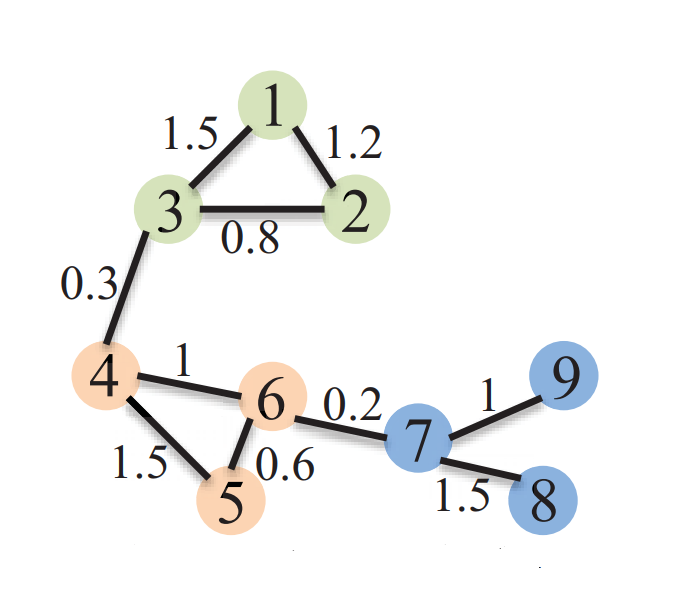
\includegraphics[width=7 cm]{images/graph_emb_1.png}
	\caption{Ví dụ về đồ thị đầu vào}
	\label{fig:graphInput}
\end{figure}

\begin{itemize}
	\item \begin{definition}[Đồ thị]\label{def:defGraph}
		\(\mathcal{G} = (V, E)\), trong đó \(v \in V\) là một đỉnh và \(e \in E\) là một cạnh. \(\mathcal{G}\) được liên kết với hàm ánh xạ loại đỉnh \(f_v: V \to T^v\) và hàm ánh xạ loại cạnh: \(f_e: E \to T^e\) .
	\end{definition}
	
	Trong đó: \(T^v\) và \(T^e\) lần lượt là tập hợp các loại đỉnh và loại cạnh. Mỗi đỉnh \(v_i \in V\) thuộc về một loại cụ thể, tức là, \(f_v(v_i) \in T^v\). Tương tự, đối với \(e_{ij} \in E, f_e (e_{ij}) \in T^e\).
	
	\item
	\begin{definition}[Đồ thị đồng nhất]\label{def:homogeneous}
		Đồ thị đồng nhất (homogeneous graph) : \textit{ $\mathcal{G}_{homo} = (V, E)$ là đồ thị trong đó $\mid T^v \mid = \mid T^e \mid = 1$. Tất cả các đỉnh trong $\mathcal{G}$ thuộc về một loại duy nhất và tất cả các cạnh thuộc về một loại duy nhất}.
	\end{definition}
	
	\item
	\begin{definition}[Đồ thị không đồng nhất]\label{def:heterogeneous}
		Đồ thị không đồng nhất (heterogeneous graph) : \textit{$\mathcal{G}_{hete} = (V, E)$ là một đồ thị trong đó $\mid T^v \mid > 1$ hoặc $\mid T^e \mid > 1$. Tức là có nhiều hơn một loại đỉnh hoặc nhiều hơn một loại cạnh}.
	\end{definition}
	
	\item
	\begin{definition}[Đồ thị tri thức]\label{def:knowledgeGraph}
		Đồ thị tri thức (knowledge graph)
		$\mathcal{G}_{know} = (V, R, E)$ là một đồ thị có hướng, có tập đỉnh là biểu diễn cho các thực thể (entities), tập quan hệ biểu diễn các mối quan hệ (relations) giữa các đỉnh, tập cạnh (edges) biểu diễn các sự kiện $E \subseteq V\times R \times V$ là gồm bộ ba subject-property-object. Mỗi cạnh là một mẫu gồm $(\text{entity}_{\text{head}}, \text{relation}, \text{entity}_{\text{tail}})$ (ký hiệu là $\langle h, r, t \rangle$) biểu thị mối quan hệ của $r$ từ thực thể $h$ đến thực thể $t$ .
	\end{definition}
	Trong đó $h, t \in V$ là các thực thể và $r \in R$ là các quan hệ. Chúng ta gọi $\langle h, r, t \rangle$ một bộ ba (triples) đồ thị tri thức.
	
	Ví dụ: trong hình \ref{fig:graphExample} có hai bộ ba: $\langle \text{Tom\ Cruise,\ born_in,\ New\ York} \rangle$ và $\langle \text{New York, state_of, U.S} \rangle$. Lưu ý rằng các thực thể và quan hệ trong đồ thị tri thức thường có các loại khác nhau. Do đó, đồ thị tri thức có thể được xem như là một ví dụ của đồ thị không đồng nhất.
\end{itemize}

\section{Dự đoán liên kết trong đồ thị tri thức}

Dự đoán liên kết (link prediction) hay hoàn thiện đồ thị tri thức (knowledge graph completion) là nhiệm vụ khai thác những sự kiện có sẵn trong đồ thị tri thức để suy luận ra sự kiện còn thiếu. Điều này tương đương với việc đoán đúng thực thể đuôi $\langle h, r, ? \rangle$ (dự đoán đuôi) hoặc $\langle ?, r, t \rangle$ (dự đoán đầu). Để đơn giản,  thay vì gọi dự đoán đầu hoặc đuôi, một cách tổng quát chúng ta gọi thực thể nguồn (source) là thực thể đã biết trong việc dự đoán, thực thể đích (target) là cái chúng ta cần dự đoán.


Hầu hết các nghiên cứu hiện tại về việc dự đoán liên kết của đồ thị tri thức đều liên quan đến các phương pháp tiếp cận tập trung vào khái niệm nhúng một đồ thị đã cho trong một không gian vectơ có số chiều thấp. Ngược lại với các tiếp cận này là một phương pháp đựa trên luật được nghiên cứu trong \cite{burl}. Thuật toán cốt lõi của nó dựa trên lấy mẫu một luật bất kỳ, sau đó khái quát  thành các quy tắc Horn\cite{wiki:Horn}. Tiếp đó dùng thống kê để tính độ tin cậy của các luật được khái quát. Khi dự đoán một liên kết mới (cạnh mới) của đồ thị chúng ta dự đoán một đỉnh có cạnh nối với một quan hệ cụ thể (label) với đỉnh còn lại hay không. Cũng đã có rất nhiều phương pháp được nghiên cứu, đề xuất để học các các luật trong đồ thị chẳng hạn như trong  RuDiK\cite{ortona2018robust}, AMIE\cite{galarraga2015fast}, RuleN\cite{meilicke2018fine}. 
Như đã nói trong phần trước có hai cách tiếp cận chính cho bài toán này một là tối ưu hóa hàm mục tiêu. Tìm ra một bộ quy tắc nhỏ bao gồm phần lớn các ví dụ là đúng và ít sai sót nhất có thể như được ngiên cứu trong RuDiK\cite{ortona2018robust}. Còn cách tiếp cận còn lại cũng là cách tiếp cận mà chúng tôi chọn nghiên cứu là cố gắng tìm hiểu mọi quy tắc khả thi có thể sau đó tạo xếp hạng \(k\) ứng viên tiềm năng với một độ tin cậy nhất định được đo trên tập huấn luyện.

Phương pháp đựa trên luật của chúng tôi phần lớn dựa vào phương pháp Anytime Bottom-Up Rule Learning for Knowledge Graph Completion \cite{meilicke2019anytime} mà sau đây chúng tôi gọi là \textbf{AnyBURL}. Như tên của phương pháp này phương pháp chủ yếu chú trọng vào vấn đề hoàn thành đồ thị, điền những phần còn thiếu vào đồ thị. Vấn đề tồn đọng lại ở mô hình này khi có một cạnh mới hay một tri thức mới được thêm vào đồ thị sẽ phải đào tạo lại toàn bộ mô hình. Chúng tôi giải quyết vẫn đề này theo hai chiến lược offline-to-online tức là khi thêm vào đồ thị tập hợp các cạnh thì mới thực hiện lại quá trình đào tạo lại một phần của đồ thị và chiến lược thứ 2 là online-to-online  khi thêm một cạnh mới sẽ thực hiện đào tạo lại ngay một phần có liên quan tới cạnh vừa thêm vào.

% GAT
Trong nhánh các phương pháp về học sâu, rất nhiều kỹ thuật học sâu thành công trong xử lý ảnh và xử lý ngôn ngữ tự nhiên được áp dụng vào đồ thị tri thức như : Mạng Neural Tích Chập (Convolution Neural Network - CNN \cite{lecun1999object}), Mạng Neural Hồi Quy (Recurrent Neural Network\cite{hopfield2007hopfield}), và gần đây như Transformer (\cite{yang2019xlnet}), Mạng Neural Bao Bọc (Capsule Neural Network - CapsNet \cite{sabour2017dynamic}). Bên cạnh đó các nghiên cứu còn sử dụng một số kỹ thuật khác như Random Walks, các mô hình dựa trên cấu trúc phân cấp, .. Ưu điểm chung của nhóm các phương pháp học sâu trên đồ thị tri thức đó là tự động rút trích các đặc trưng và có thể khái quát hóa cấu trúc phức tạp của đồ thị dựa trên một lượng lớn dữ liệu huấn luyện. Tuy nhiên, một số phương pháp chỉ chủ yếu tập trung vào cấu trúc dạng lưới mà không giữ được đặc trưng không gian của đồ thị tri thức. 
Cơ chế chú ý hay lớp chú ý đa đỉnh (multi-head attention layer) đã được áp dụng vào đồ thị bằng mô hình Mạng Đồ Thị Chú Ý (Graph Attention Network - GAT \cite{velivckovic2017graph}) giúp tổng hợp thông tin của một thực thể dựa vào trọng số chú ý của thực thể gốc đối với các thực thể lân cận. Tuy nhiên, mô hình đồ thị chú ý lại thiếu thông tin của vector nhúng quan hệ cũng như các vector nhúng lân cận của một thực thể gốc, một phần rất quan trọng giúp thể hiện vai trò của từng thực thể. Vấn đề đó đã được giải quyết trong báo cáo Learning Attention-based Embeddings for Relation Prediction in
Knowledge Graphs (\textbf{KBAT} \cite{nathani2019learning}), mô hình được chúng tôi chọn làm cơ sở nghiên cứu.
Cơ chế chú ý đang là một trong những cấu trúc học sâu đạt được hiệu quả nhất hiện nay (state-of-the-art) vì nó đã được chứng minh là thay thế cho bất kỳ phương pháp tính tích chập nào \cite{cordonnier2019relationship},
hơn nữa nó cũng nằm trong cấu trúc cơ bản để áp dụng trên các mô hình mới nhất trên ngôn ngữ tự nhiên như mô hình Megatron-LM \cite{shoeybi2019megatron}, và trên phân đoạn hình ảnh như mô hình HRNet-OCR (Hierarchical Multi-Scale Attention \cite{tao2020hierarchical}). Một số phương pháp thú vị \cite{cordonnier2020multi} đã cải tiến dựa trên cơ chế chú ý, tuy nhiên nó lại chưa được áp dụng vào đồ thị tri thức, vì vậy chúng tôi chọn nhóm phương pháp này để áp dụng các cải tiến mới nhất vào đồ thị tri thức.

\section{Các lĩnh vực nghiên cứu về đồ thị tri thức}

\begin{figure}[htp]
	\centering
	\tikzset{
		category/.style  = {draw, font=\sffamily, thin, align=center},
		subcat/.style={rectangle, rounded corners=6pt},
		center/.style = {category, ellipse, fill=blue!60, text width=4em},
		group/.style = {category, subcat, fill=blue!30, rounded corners=6pt, text width=6em},
		yellowbox/.style = {category, subcat, fill=yellow!30},
		greenbox/.style = {category, subcat, fill=green!30},
		redbox/.style = {category, subcat, fill=red!30},
		bluebox/.style = {category, subcat, fill=cyan!30},
		leafbox/.style = {category, subcat, fill=black!10, rounded corners=0mm}
	}
	\resizebox{\textwidth}{!}{%
		\begin{tikzpicture}
			\node[center] (root) {Đồ thị tri thức};
			\node[group][above left=1cm of root] (c1) {Học biểu diễn tri thức};
			\node[group][above right=8mm of root] (c2) {Nhận biết tri thức};
			\node[group][below left=5mm of root] (c3) {Thu nhận tri thức};
			\node[group][below right=20mm of root, xshift=-2cm] (c4) {Đồ thị tri thức thời gian};
			
			\begin{scope}[every node/.style={yellowbox}]
				\node[above=8mm of c1, xshift=-1cm] (c11) {Biểu diễn không gian};
				\node[left=of c1, yshift=9mm, xshift=-10mm] (c12) {Hàm đánh giá};
				\node[left=15mm of c1, yshift=-5mm] (c13) {Mã hóa mô hình};
				\node[left=of c1, yshift=-20mm] (c14) {Thông tin tương tự};
			\end{scope}
			
			\begin{scope}[every node/.style={redbox}]
				\node[above left=of c2, text width=35mm, yshift=1mm, xshift=18mm] (c21) {Hiểu ngôn ngữ tự nhiên};
				\node[above=1cm of c2, yshift=5mm, xshift=13mm] (c22) {Trả lời câu hỏi};
				\node[right=of c2, yshift=15mm] (c23) {Hệ thống hội thoại};
				\node[right=of c2, yshift=-2mm] (c24) {Hệ thống gợi ý};
				\node[below=5mm of c2, xshift=5mm] (c25) {Ứng dụng khác};
			\end{scope}
			
			\begin{scope}[every node/.style={greenbox}]
				\node[left=1cm of c3, yshift=5mm] (c31) {Khai phá thực thể};
				\node[below left=of c3, yshift=1cm, xshift=3mm] (c32) {Rút trích quan hệ};
				\node[below right=5mm of c3, xshift=-4cm] (c33) {Hoàn thiện đồ thị};
			\end{scope}
			
			\begin{scope}[every node/.style={bluebox}]
				\node[below=of c4, xshift=-15mm, yshift=-35mm] (c41) {Lý giải logic thời gian};
				\node[below=of c4, xshift=2cm, yshift=-23mm] (c42) {Quan hệ thời gian độc lập};
				\node[below right=of c4,xshift=-2mm, yshift=-10mm] (c43) {Thực thể động};
				\node[right=of c4, yshift=-2cm, xshift=15mm] (c44) {Nhúng thời gian};
			\end{scope}
			
			\begin{scope}[every node/.style={leafbox}]
				\node[above=5mm of c11] (c11x) {
					\begin{tabular}{@{}l@{}@{}l@{}}
						-Point-wise & -Đa tạp \\
						-Số phức & -Gausian \\
						-Rời rạc & \\
					\end{tabular}
				};
				\node[above=5mm of c12, xshift=-5mm] (c12x) {
					\begin{tabular}{@{}l@{}}
						-Khoảng cách \\
						-Ngữ nghĩa \\
						-Khác \\
					\end{tabular}
				};
				\node[left=of c13, yshift=5mm] (c13x) {
					\begin{tabular}{@{}l@{}}
						-Tuyến tính/ \\song tuyến tính \\
						-Ma trận hóa \\
						-Neural Nets \\
						-CNN \\
						-RNN \\
						-Transformers \\
						-GCN \\
					\end{tabular}
				};
				\node[below left=5mm of c14, xshift=6mm, yshift=-7mm] (c14x) {
					\begin{tabular}{@{}l@{}c@{}l@{}}
						-Văn bản & -Kiểu & -Trực quan \\
					\end{tabular}
				};
				%%%%%%%%%%%% 
				\node[below left=of c31] (c31x) {
					\begin{tabular}{@{}l@{}}
						-Nhận dạng \\
						-Định kiểu \\
						-Phân biệt \\
						-Sắp xếp \\
					\end{tabular}
				};
				\node[below=of c32, xshift=-5mm] (c32x) {
					\begin{tabular}{@{}l@{}}
						-Neural Nets\\
						-Chú ý \\
						-GCN \\
						-GAN \\
						-RL \\
						-Khác \\
					\end{tabular}
				};
				\node[below=5mm of c33] (c33x) {
					\begin{tabular}{@{}l@{}}
						-Nhúng dựa trên xếp hạng\\
						-Lý giải đựa trên đoạn \\
						-Lý giải dựa trên luật \\
						-Học siêu quan hệ \\
						-Phân loại bộ ba \\
					\end{tabular}
				};
				%%%%%%%%%%%%%%%%%
				\node[above=5mm of c22] (c22x) {
					\begin{tabular}{@{}l@{}}
						-Single-fact QA\\
						-Lý giải nhiều bước \\
					\end{tabular}
				};
				\node[below right=5mm of c25, yshift=15mm] (c25x) {
					\begin{tabular}{@{}l@{}}
						-Sinh câu hỏi\\
						-Công cụ tìm kiếm \\
						-Ứng dụng y khoa \\
						-Hồi phục sức khỏe \\
						-Phân loại ảnh zero-shot\\
						-Sinh văn bản\\
						-Phân tích ngữ nghĩa\\
					\end{tabular}
				};
				
			\end{scope}
			
			\foreach \value in {1,...,4}
			\draw[->, line width=0.8mm] (root) -> (c\value);
			
			\foreach \value in {1,...,4}
			\draw[->, ultra thick] (c1) -> (c1\value);
			\foreach \value in {1,...,4}
			\draw[->, thick] (c1\value) -> (c1\value x);
			
			\foreach \value in {1,...,5}
			\draw[->, ultra thick] (c2) -> (c2\value);
			\foreach \value in {2,5}
			\draw[->, thick] (c2\value) -> (c2\value x);
			
			\foreach \value in {1,...,3}
			\draw[->, ultra thick] (c3) -> (c3\value);
			\foreach \value in {1,...,3}
			\draw[->, ultra thick] (c3\value) -> (c3\value x);
			
			\foreach \value in {1,...,4}
			\draw[->, ultra thick] (c4) -> (c4\value);
			
	\end{tikzpicture}}
	\caption{
		Danh mục các lĩnh vực nghiên cứu trên đồ thị tri thức}
	\label{fig:categoriesResearch}
\end{figure}

Biểu diễn tri thức đã từng có lịch sử phát triển suốt chiều dài lịch sử trong lĩnh vực logic và trí tuệ nhân tạo. Trên đồ thị tri thức, có 4 bốn nhóm nghiên cứu chính đã được phân loại và tổng hợp ở báo cáo \cite{ji2020survey} bao gồm : Học Biểu Diễn Tri Thức (Knowledge Representation Learning), Thu Nhận Tri Thức (Knowledge Acquisition), Đồ Thị Tri Thức Về Thời Gian (Temporal Knowledge Graphs), Ứng Dụng Nhận Biết Tri Thức (Knowledge-aware Applications). Tất cả các danh mục nghiên cứu được minh họa ở hình \ref{fig:categoriesResearch}.

\textbf{Học biểu diễn tri thức}

Học biểu diễn tri thức là vấn đề tìm hiểu thiết yếu của đồ thị tri thức giúp mở ra rất nhiều ứng dụng trong thực tế. Học biểu diễn tri thức được phân loại thành bốn nhóm con bao gồm : 

\begin{itemize}
	\item \textit{Biểu Diễn Không Gian} (Representation Space) nghiên cứu về cách các thực thể và quan hệ được biểu diễn trong không gian. Biểu diễn không gian bao gồm không gian điểm (point-wise), đa tạp (manifold), không gian vector số phức (complex), phân phối Gaussian và không gian rời rạc.
	
	\item \textit{Hàm Đánh Giá} (Scoring Function) nghiên cứu về hàm đo lường giá trị của một bộ ba trong thực tế, bao gồm các hàm đánh giá dựa trên khoảng cách hoặc dựa trên sự tương đồng.
	
	\item \textit{Mã Hóa Mô Hình} (Encoding Models) nghiên cứu về cách biểu diễn và học các tương tác giữa các mối quan hệ. Đây là hướng nghiên cứu chính hiện nay, bao gồm các mô hình tuyến tính hoặc phi tuyến tính, phân rã ma trận hoặc mạng neural.
	
	\item \textit{Thông Tin Bổ Trợ} (Auxiliary Information) nghiên cứu về cách kết hợp vào các phương pháp nhúng, các thông tin bổ trợ bao gồm văn bản, hình ảnh và loại thông tin .
\end{itemize}

\textbf{Thu nhận tri thức}

Thu nhận tri thức nghiên cứu về cách thu nhận tri thức dựa trên đồ thị tri thức, bao gồm hoàn thiện đồ thị (knowledge graph completion), khai thác quan hệ và khai phá thực thể. Khai thác quan hệ và khai phát thực thể là nhóm phương pháp khai thác tri thức mới (bao gồm các quan hệ hoặc thực thể) trong đồ thị từ văn bản. Hoàn thiện đồ thị là nhiệm vụ mở rộng đồ thị tri thức dựa trên đồ thị đang có. Hoàn thiện đồ thị bao gồm các hướng nghiên cứu như : xếp hạng dựa trên nhúng (embedding-based ranking), dự đoán đường đi quan hệ (relation path reasoning), dự đoán dựa trên luật (rule-based reasoning) và học siêu quan hệ.
Khai phá thực thể bao gồm nhận dạng, phân biệt, định kiểu và sắp xếp. 
Các mô hình khai thác quan hệ sử dụng cơ chế chú ý, mạng đồ thị tích chập (graph
convolutional networks), huấn luyện đối nghịch (adversarial training), học tăng cường (reinforcement learning), học sâu và học chuyển tiến (transfer learning), đây là hướng nghiên cứu trong phương pháp đề xuất của chúng tôi.

Ngoài ra, trên đồ thị tri thức còn có các hướng nghiên cứu như \textbf{đồ thị tri thức về thời gian} và \textbf{ứng dụng nhận biết tri thức}. Đồ thị tri thức về thời gian sẽ kết hợp thêm thông tin thời gian trên đồ thị để học cách biểu diễn, còn ứng dụng nhận biết tri thức bao gồm hiểu ngôn ngữ tự nhiên (natural language understanding), trả lời câu hỏi (question answering), hệ thống gợi ý (recommendation systems) và nhiều nhiệm vụ khác trong thế giới thực mà nó tích hợp tri thức vào để cải thiện quá trình học biểu diễn .
\chapter{Phương pháp dựa trên luật}
\label{chap:RuleBase}

Trong phần này chúng tôi mô tả lại cách mô hình hóa lại bài toán theo phương pháp dựa trên luật AnyBURL,thuật toán lấy mẫu luật (đường đẫn) và thuật toán khái quát hóa một luật để lưu trữ trở thành tri thức của mô hình. Cùng với những cải tiến của chúng tôi trong quá trình đào tạo khi có một tri thức mới được thêm vào đồ thị(thêm cạnh).

\section{Luật Horn}
Trong logic toán học, một công thức nguyên tử (\textbf{atomic formula})\cite{wiki:Atomic} còn được gọi đơn giản là một (nguyên tử-\textbf{atom}) là một công thức không có cấu trúc mệnh đề, nghĩa là một công thức không chứa các liên kết logic (\(\vee, ~ \wedge\)) hoặc tương đương (\(\Leftrightarrow\)) là một công thức không có các mẫu con nghiêm ngặt (tức là atom không thể chia nhỏ ra thành các atom con nữa). Do đó, các công thức nguyên tử là công thức đơn giản nhất để hình thành luật của logic. Các công thức hợp được hình thành bằng cách kết hợp các công thức nguyên tử bằng cách sử dụng các liên kết logic.

Một \textbf{literal}\cite{wiki:Literal} là một công thức nguyên tử (atom) hoặc phủ định của nó. Định nghĩa chủ yếu xuất hiện trong lý thuyết logic cổ điển. \textbf{Literal} có thể được chia thành hai loại: Một \textbf{positive literal} chỉ là một nguyên tử (ví dụ: \(x\)). Một \textbf{negative literal} là phủ định của một nguyên tử (ví dụ: \(\neg x\)). Sự phân chia của \textbf{literal} là \textbf{positive literal} hay \textbf{negative literal} tùy thuộc vào việc \textbf{literal} được định nghĩa.

Một mệnh đề (clause) là một literal hoặc nối rời của hai hoặc nhiều literal. Ở dạng \textbf{Horn} một mệnh đề có nhiều nhất một positive literal. Lưu ý: Không phải mọi công thức trong logic mệnh đề đều có thể đưa về dạng Horn.Mệnh đề xác định không có literal đôi khi được gọi là mệnh đề đơn vị (unit clause) và một mệnh đề đơn vị không có biến đôi khi được gọi là \textit{facts}\cite{wiki:Horn}.Một công thức nguyên tử được gọi là \textit{ground} hoặc \textit{ground atoms} nếu nó được xây dựng hoàn toàn từ các mệnh đề đơn vị; tất cả các \textit{ground atoms} có thể ghép lại từ một tập hợp hàm và các ký hiệu vị từ nhất định tạo nên cơ sở Herbrand cho các bộ ký hiệu này\cite{wiki:Term}.

\section{Định nghĩa ngôn ngữ đồ thị  tri thức} \label{kg}

Khác với các định nghĩa về đồ thị tri thức tổng quát được đùng cho các phương pháp nhúng đồ thị. Trong phương pháp dựa trên luật của chúng tôi. Chúng tôi xem đồ thị như là một ngôn ngữ hình thức. Dưới đây là các định nghĩa theo ngôn ngữ hình thức của đồ thị tri thức.

Một đồ thị tri thức \(\mathbb{G}\) được định nghĩa trên một bộ từ vựng \(\langle \mathbb{C}, \mathbb{R} \rangle\) trong đó \(\mathbb{C}\) là tập hợp các hằng số và \(\mathbb{R}\) là tập hợp các vị từ nhị phân.Khi đó, \(\mathbb{G} = \{r (a, b) \mid r \in \mathbb{R}, a, b \in \mathbb{C}\}\) là tập hợp các \textit{ground atoms} hoặc \textit{facts}. Một vị từ nhị phân được gọi là quan hệ và hằng số (hoặc hằng số được đề cập đến) được gọi là thực thể (entity) tương ứng với một dòng dữ liệu trong tập huấn luyện. Sau đây chúng tôi sử dụng các chữ cái viết thường cho các hằng và chữ in hoa cho các biến cho các thảo luận dưới đây. Vì chúng ta không học các quy tắc Horn tùy ý, và chỉ học đối với loại quy tắc nào có thể được khái quát hóa như được thảo luận dưới đây.

Chúng ta định nghĩa một quy tắc là \(h(c_0, c_n) \gets b_1(c_0, c_1) ,\dots ,b_n(c_{n}, c_{n + 1})\) là một đường dẫn ground atoms có chiều dài \(n\). Trong đó \(h(\dots)\) được gọi là \textit{head atoms} và \( b_1(c_0, c_1) ,\dots ,b_n(c_{n}, c_{n + 1})\) được gọi là \textit{body atoms}. Chúng tôi sẽ phân biệt dưới đây ba loại quy tắc mà chúng tôi gọi là: \textit{quy tắc nhị phân} \((\mathbf{B})\) là quy tắc trong head atoms chứa 2 biến, quy tắc đơn nguyên kết thúc bằng một đỉnh treo  và atom này chỉ chứa biến không chứa hằng số\((\mathbf{U_d})\) và head atoms chỉ chứa 1 biến. Còn quy tắc đơn nguyên kết thúc bằng một atom \((\mathbf{U_c)}\) và head atoms cũng chỉ chứa 1 biến.\((\mathbf{U_c)}\)  có thể là một đỉnh treo tới một hằng số bất kì nếu hằng số này trùng mới hằng số trong head atom thì tạo thành một đường đẫn có chu trình.

\[B \hspace{3.7cm} h(A_0,A_n) \gets  \bigwedge^n_{i=1} b_i(A_{i-1}, A_i)\]
\[U_d \hspace{3.8cm} h(A_0,c) \gets  \bigwedge^n_{i=1} b_i(A_{i-1}, A_i)\]
\[U_c \hspace{1cm} h(A_0,c) \gets  \bigwedge^{n-1}_{i=1} b_i(A_{i-1}, A_i) \wedge b_n(A_{n-1}, c^{\prime})\]

Chúng tôi gọi các quy tắc của các loại này là quy tắc đường đi (path rules), bởi vì các body atoms (phần sau đấu \(\gets\)) tạo thành một đường đi. Lưu ý rằng nó cũng bao gồm các biến thể quy tắc với các biến được đảo ngược trong các nguyên tử: được đưa ra trong đồ thị tri thức \(\mathbb{G}\), đường dẫn có độ dài \(n\) là một chuỗi gồm \(n\) bộ ba \(p_i (c_i, c_i + 1)\) với \(p_i (c_i, c_i + 1) \in \mathbb{G}\) hoặc \(p_i (c_i + 1, c_i) \in \mathbb{G}\) với \(0 \geq i \leq n\). Các mẫu quy tắc trừu tượng (abstract rule patterns) được cho ở trên có độ dài \(n\) vì body atoms của chúng có thể được khởi tạo thành một đường dẫn có độ dài \(n - 1\). Ví dụ như \hyperref[fig:burl]{hình 3.1}. Khi lấy mẫy đường đãn với độ dài bằng 3 chúng ta có thể có hai quy tắc sau: Quy tắc được đánh đấu màu xanh lá cây và quy tắc được đánh dấu màu đỏ 
\[speaks(ed, d) \gets married(ed, lisa) \wedge born(lisa, a) ~~~ \text{(xanh lá cây)}\]
\[\hspace{0.7cm}speaks(ed, d) \gets lives(ed, nl) \wedge lang(nl, d) ~~~ \text{(đỏ)} \]

\begin{figure*}[htp]
	\centering
	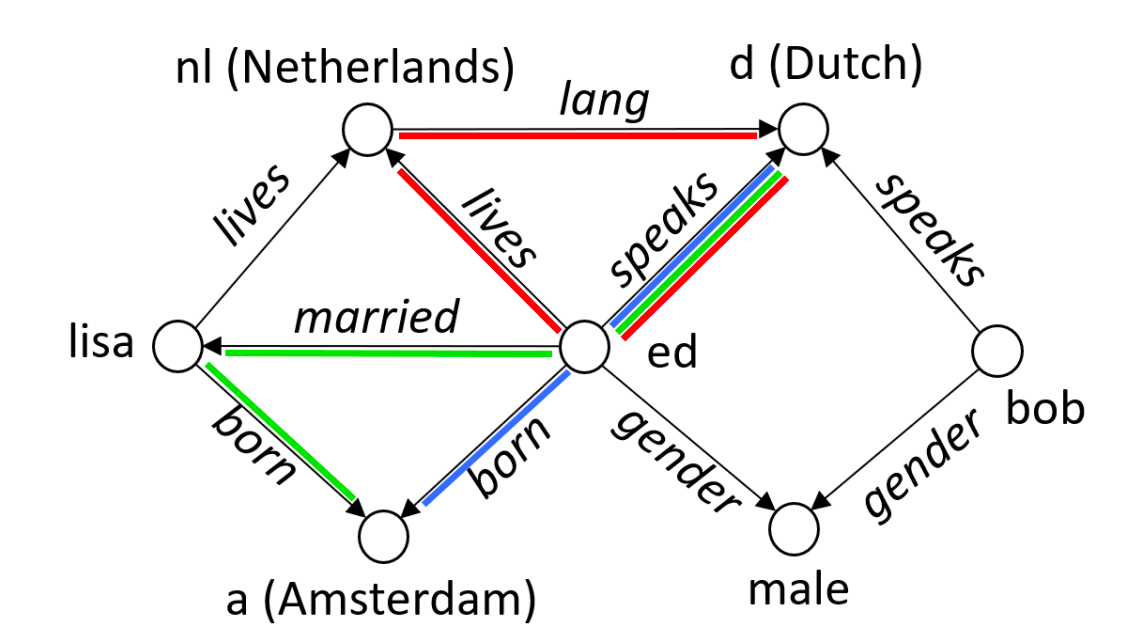
\includegraphics[width=12cm]{burl-ago.png}
	\caption{Ví dụ đồ thị tri thức}
	\label{fig:burl}
\end{figure*}

Ngoài ra Quy tắc \(B\) và quy tắc \(U_c\) cũng được gọi là quy tắc kết nối kín. Chúng có thể được học bởi hệ thống khai thác AMIE được mô tả trong \cite{AMIE,galarraga2015fast}. Quy tắc \(U_d\) là quy tắc không đóng hay đường đi không tạo thành chu trình vì \(A_n\) là biến chỉ xuất hiện một lần. Ví dụ:
\[
\begin{matrix}
	\textit{speaks}(X, Y ) & \gets & \textit{lives}(X, Y) & \quad (1) \\
	\textit{lives\_in\_city}(X, Y ) & \gets & \textit{lives}(X, A),\textit{within}(Y, A)  & \quad  (2) \\
	\textit{gen}(X, female) & \gets & \textit{married}(X, A), \textit{gen}(A, male)  & \quad  (3) \\
	\textit{profession}(X, actor) &  \gets & \textit{acted\_in}(X, A)  & \quad (4)
\end{matrix}
\]
Quy tắc (1) là quy tắc \textbf{B}(quy tắc nhị phân) quy tắc này nói rằng nếu một người (thực thể) \(X\) nói nguôn ngữ \(Y\) nếu người \(X\) sống  ở đất nước \(Y\).Rõ ràng quy tắc này là một quy tắc khái quát miễn khi nào thực thể \(X\) có cạnh nối với thực thể \(Y\) với nhãn là \textit{lives} thì có thể kết thêm 1 cạnh với nhãn \textit{speaks} giữa \(X\) và \(Y\). Quy tắc (2), (3) điều là quy tắc \(U_c\) ,quy tắc (2) nói rằng người \(X\) sống ở thành phố \(Y\) nếu người \(X\) sống ở quốc gia \(A\) và thành phố \(Y\) nằm trong quốc gia \(A\), quy tắc (3) nói rằng nếu một người \(X\) là nữ nếu họ kết hôn với một người \(A\) và người \(A\) có giới tính nam. Ở quy tắc (3) không tạo thành chu trình trên đồ thị như quy tắc (2) đỉnh (Y) lặp lại  ở \textit{head atom} và đỉnh cuối cùng trong \textit{body atoms}. Quy tắc (4) là quy tắc \(U_d\) nói rằng người \(X\) là một điễn viên nếu người \(X\) đóng trong một bộ phim \(A\).

Tất cả các quy tắc được xem xét sẽ được lọc lại đựa trên điểm được gọi là độ tin cậy của quy tắc là được đo trên tập dữ liệu huấn luyện. Độ tin cậy này được đo bằng tỷ lệ body atoms dẫn đến head atoms chia cho tất cả các đường đẫn chứa body atoms.Ví dụ khi ta có quy tắc sau:
\(\textit{gen}(X, female) \gets \textit{married}(X, A), \textit{gen}(A, male) \). Khi đó chúng ta thực hiện đếm tất cả các cặp thực thể có quan hệ  \(\textit{married}(X, A), \textit{gen}(A, male) \) được gọi là số đường dẫn chứa body atoms, sau đó thực hiện đếm tất cả các  thực thể thỏa quan hệ \(\textit{gen}(X, female) \gets \textit{married}(X, A), \textit{gen}(A, male) \) được gọi là số body atoms dẫn đến head atoms. Sau đó chia số body atoms dẫn đến head atoms cho  đường dẫn chứa body atoms được gọi là độ tin cậy của quy tắc.

\section{Thuật toán AnyBURL} \label{myalgorithm}
Trong phần này chúng tôi mô tả lại thuật toán chính của phương pháp AnyBURL nó cũng được mô tả trong \cite{burl} cũng như hai thuật toán mở rộng của chúng tôi để giải quyết vấn đề khi đồ thị được thêm một hoặc một lượng tri thức mới (thêm cạnh). Ngoài ra chúng tôi cũng mô tả sơ lược lại cách khởi tạo một luật cũng như cách thức tính toán độ tin cậy bằng cách lấy mẫu trên tập huấn luyện và vấn đề độ tin cậy khi dự đoán một luật khi tính toán độ tin cậy bằng việc lấy mẫu.
\subsection{AnyBURL}
\begin{algorithm}
	\caption{Anytime Bottom-up Rule Learning}\label{algorithm1}
	\begin{algorithmic}[1]
		\Procedure{AnyBURL($\mathbb{G}$, s, sat, Q, ts)}{}
		\State $\textit{n} = \text{2}$
		\State $R = \emptyset$
		\Loop
		\State $R_s = \emptyset$
		\State $start = currentTime()$
		\Repeat
		\State $p = samplePath(\mathbb{G}, n)$
		\State $R_p = generateRules(p)$
		\For {$r \in R_p$}
		\State $score(r, s)$
		\If {$Q(r)$}
		\State $R_s = R_s \cup \{r\}$
		\EndIf
		\EndFor
		\Until {$currentTime() > start + ts$}
		\State $R^{\prime}_s = R_s \cap R$
		\If {$ \mid R^{\prime} \mid / \mid R \mid > SAT$}
		\State $n = n + 1$
		\EndIf
		\State $R = R_s \cap R$
		\EndLoop
		\Return R
		\EndProcedure
	\end{algorithmic}
\end{algorithm}

Đầu vào của thuật toán \(\mathbb{G}, S, SAT, Q, TS\). Đầu ra là tập hợp \(R\) các luật học được. Trong đó \(\mathbb{G}\) là một đồ thị tri thức được cho từ tập dữ liệu đào tạo. \(S\) là tham số cho biết kích thước của một lần lấy mẫu trên dữ liệu đào tạo để tính toán độ tin cậy. \(SAT\) cho biết độ bão hòa(saturation) của các luật được sinh ra trong 1 lần lặp độ bão hòa này được tính bằng số luật \textbf{mới} học được ở lần lặp hiện tại so với số luật đã học được. Nếu nhỏ hơn độ bão hòa thì chúng tôi cho rằng vẫn còn tiềm năng để khai thác các luật với độ dài \(n\). Ngược lại chúng tôi tăng độ dài của luật sau đó tiếp tục khai thác. \(Q\) là một ngưỡng để xác định xem luật mới được sinh ra có được thêm vào kết quả trả về hay không. Còn \(TS\) cho biết thời gian học của thuật toán. Chúng tôi bắt đầu với \(n\) bằng \(2\) tức là các luật có độ dài đường đẫn bằng 2 vì trong path rule yêu cầu ít nhất 1 literal trong head atom và 1 trong body atoms. Ở phần lấy mẫu 1 luật(\textit{samplePath}) chỉ đơn giản là chúng ta chọn một đỉnh bất kì trong đồ thị duyệt qua tất cả các đường đẫn từ đỉnh đó đi qua \(n\) đỉnh khác, sau đó chọn ngẫu nhiên một đường đẫn trong số các trường đẫn duyệt được.

\subsection{Tạo luật}
\begin{algorithm}
	\caption{Generate Rules(p)}\label{algorithm2}
	\begin{algorithmic}[1]
		\Procedure{generate\_rules(p)}{}
		\State $\textit{generalizations} = \emptyset$
		\State $is\_binary\_rule = random.choices([true,false])$
		\If {$is\_binary\_rule$}
		\State $replace\_all\_head\_by\_variables(p)$
		\State $replace\_all\_tail\_by\_variables(p)$
		\State $add(generalizations, p)$
		\Else:
		\State $replace\_all\_head\_by\_variables(p)$
		\State $add(generalizations, p)$
		\State $replace\_all\_tail\_by\_variables(p)$
		\State $add(generalizations, p)$
		\EndIf
		\Return $generalizations$
		\EndProcedure
	\end{algorithmic}
\end{algorithm}

Ở thuật toán này chúng tôi thay các hằng số vào các head và tail trong toàn bộ path rule  của luật được lấy mẫu ở bước trước nếu luật cần học là luật nhị phân ngược lại chúng tôi chỉ thay hoặc head hoặc tail rồi thêm vào luật trả về sau đó chúng tôi lấy mẫu trên tập huấn luyện 1 tập hợp các luật sau đó tính toán độ tin cây như được mô tả trong phần \hyperref[kg]{2.3.2}. Để giảm chi phí tính toán chúng tôi chọn cách lấy mẫu trên tập huấn luyện để tính toán. Khi đưa ra dự đoán các ứng cử viên của một luật chúng tôi sẽ tính toán lại bằng cách thêm vào một lượng biểu diễn số luật bị sai mà chúng tôi chưa nhìn thấy trong quá trình lấy mẫu để tính toán độ tin cậy. Đối với mô hình của chúng thôi sau khi thử nghiệm tham số trong khoảng \([5, 10]\) cho kết quả tốt nhất.
\section{Thuật toán AnyBURL mở rộng}
\subsection{Thuật toán 3 học offline-to-online}

\begin{algorithm}
	\caption{AnyBURL Learning batch size}\label{algorithm3}
	\begin{algorithmic}[1]
		\Procedure{AnyBURLbatch($\mathbb{G}$, s, sat, Q, ts, batch\_edge)}{}
		\State $is\_connected = add(\mathbb{G}, batch\_edge)$
		\If {$is\_connected$}
		\State  $ G^{\prime} = \mathbb{G} \oplus batch\_edge$
		\Else
		\State  $ G^{\prime} = batch\_edge$
		\EndIf
		\State $\textit{n} = \text{2}$
		\State $R = \emptyset$
		\Loop
		\State $R_s = \emptyset$
		\State $start = currentTime()$
		\Repeat
		\State $p = samplePath(batch\_edge, n)$
		\State $R_p = generateRules(p)$
		\For {$r \in R_p$}
		\State $score(r, s)$
		\If {$Q(r)$}
		\State $R_s = R_s \cup \{r\}$
		\EndIf
		\EndFor
		\Until {$currentTime() > start + ts$}
		\State $R^{\prime}_s = R_s \cap R$
		\If {$ \mid R^{\prime} \mid / \mid R \mid > SAT$}
		\State $n = n + 1$
		\EndIf
		\State $R = R_s \cap R$
		\EndLoop
		\Return R
		\EndProcedure
	\end{algorithmic}
\end{algorithm}

Thuật toán này là phần bổ xung của chúng tôi để tránh việc phải đào tạo lại toàn bộ mô hình khi có một lượng tri thức mới được thêm vào đồ thị. Khi thêm vào đồ thị chúng tôi kiểm trả xem phần tri thức mới có kết nối với tri thức cũ hay không (tính liên thông) nếu có chúng tôi thực hiện phép toán \(\oplus\) lấy  tất cả các phần trong \(batch\_edge\) thêm với 1 phần liên thông với những cạnh liên thông với đồ thị với dộ dài là \(5\), Nếu không chúng tôi lấy tất cả các phần trong \(batch\_edge\) sau đó thực hiện lại các bước như thuật toán Anytime Bottom-up Rule Learning.

\subsection{Thuật toán 4 học online-to-online}
\begin{algorithm}
	\caption{AnyBURL Learning batch size}\label{euclid}
	\begin{algorithmic}[1]
		\Procedure{AnyBURLbatch($\mathbb{G}$, s, sat, Q, ts, edge)}{}
		\State $is\_connected = add(\mathbb{G}, edge)$
		\State $R = \emptyset$
		\If {$is\_connected$}
		\State $\textit{n} = \text{2}$
		\State $R_s = \emptyset$
		\Repeat
		\State $p = samplePath(edge, n)$
		\State $R_p = generateRules(p)$
		\For {$r \in R_p$}
		\State $score(r, s)$
		\If {$Q(r)$}
		\State $R_s = R_s \cup \{r\}$
		\EndIf
		\EndFor
		\Until {$currentTime() > start + ts$}
		\State $R^{\prime}_s = R_s \cap R$
		\If {$ \mid R^{\prime} \mid / \mid R \mid > SAT$}
		\State $n = n + 1$
		\EndIf
		\State $R = R_s \cap R$
		\State \Return R
		\EndIf
		\EndProcedure
	\end{algorithmic}
\end{algorithm}

Thuật toán này là một phần bổ xung cho thuật toán 3 ở trên. Sở dĩ chúng tôi gọi là online-to-online là vì khi có một cạnh mới(tri thức mới) được thêm vào đồ thị chúng tôi sẽ thực hiện việc học ngay tức khắc trên các path rule liên quan tới cạnh đó không giống như ở thuật toán 3 khi có đủ 1 lượng tri thức mới được thêm vào.


%\chapter{METHOD PROPOSAL}
%\label{chap:Chapter3}
\chapter{DEEP LEARNING-BASED METHODS}
\label{chap:DeeLearning}

In this chapter, we present Knowledge Graphs and describe the task of Graph Embedding, providing an overview of current graph embedding techniques. We will revisit the attention mechanism and explain how it is applied to knowledge graphs through the Graph Attention Network (GAT) model \cite{velivckovic2017graph}. Additionally, we present an improved method based on the graph attention model—KBGAT \cite{nathani2019learning}—which incorporates relation information and neighboring relations.

\section{Graph Embedding}
\label{sec:graphEmbedding}

In the real world, representing entities and relations as vectors can be intuitively understood as the process of mapping features and attributes of an object into a lower-dimensional space, with each component representing a specific unit-level feature.

For example, we know Donald Trump is 1.9 meters tall and has a wife named Melania. Thus, we could represent the entity "Donald Trump" as a vector:

\[
\overrightarrow{e_\text{Trump}} = [1.9_{\text{height}}, 0_{\text{area}}, 1_{\text{wife is Melania}}, 0_{\text{wife is Taylor}}].
\]

For features that cannot be measured or have no value (e.g., \texttt{.area}), we assign 0. For categorical features without magnitude (e.g., \texttt{.wife}), we represent them using probabilities of unit features (e.g., \texttt{.wife is Melania}, \texttt{.wife is Taylor}). Therefore, any object in the real world can be \textit{embedded} as a vector in an interpretable way.

To understand graph embedding techniques, we begin with several fundamental definitions:

\begin{itemize}
	\item
	\begin{definition}[First-Order Proximity]\label{def:firstOrderProximity}
		First-order proximity between vertex \(v_i\) and vertex \(v_j\) is the edge weight \(A_{i, j}\) of the edge \(e_{ij}\).
	\end{definition}
	
	Two vertices are more similar if they are connected by an edge with a higher weight. Thus, the first-order proximity between \(v_i\) and \(v_j\) is denoted as \(s^{(1)}_{ij} = A_{i, j}\). Let \(s^{(1)}_i = \begin{bmatrix} s^{(1)}_{i1}, s^{(1)}_{i2}, \dots, s^{(1)}_{i|V|} \end{bmatrix}\) represent the first-order proximities between \(v_i\) and other vertices.
	
	Using the graph in \autoref{fig:graphInput} as an example, the first-order proximity between \(v_1\) and \(v_2\) is the weight of edge \(e_{12}\), denoted as \(s^{(1)}_{12} = 1.2\). The vector \(s^{(1)}_1\) records the edge weights connecting \(v_1\) to all other vertices in the graph, i.e.,
	
	\[
	s^{(1)}_{1} = \begin{bmatrix} 0, 1.2, 1.5, 0, 0, 0, 0, 0, 0 \end{bmatrix}.
	\]
	
	\item
	\begin{definition}[Second-Order Proximity]\label{def:secondOrderProximity}
		Second-order proximity \(s^{(2)}_{ij}\) between vertex \(v_i\) and \(v_j\) is defined as the similarity between \(v_i'\)'s first-order neighborhood vector \(s^{(1)}_i\) and \(v_j'\)'s vector \(s^{(1)}_j\).
	\end{definition}
	
	For example, in \autoref{fig:graphInput}, the second-order proximity \(s^{(2)}_{12}\) is the similarity between \(s^{(1)}_1\) and \(s^{(1)}_2\). As introduced above:
	
	\[
	s^{(1)}_1 = \begin{bmatrix} 0, 1.2, 1.5, 0, 0, 0, 0, 0, 0 \end{bmatrix}, \quad s^{(1)}_2 = \begin{bmatrix} 1.2, 0, 0.8, 0, 0, 0, 0 , 0, 0 \end{bmatrix}.
	\]
	
	We compute the cosine similarity:
	
	\[
	s^{(2)}_{12} = \cos(s^{(1)}_1, s^{(1)}_2) = 0.43, \quad s^{(2)}_{15} = \cos(s^{(1)}_1, s^{(1)}_5) = 0.
	\]
	
	We observe that the second-order proximity between \(v_1\) and \(v_5\) is 0 because they share no common 1-hop neighbors. \(v_1\) and \(v_2\) share a common neighbor \(v_3\), thus their second-order proximity \(s^{(2)}_{12}\) is greater than 0.
	
	Higher-order proximities can be defined similarly. For example, the \(k\)-th order proximity between \(v_i\) and \(v_j\) is the similarity between \(s^{(k-1)}_i\) and \(s^{(k-1)}_j\).
	
	\item
	\begin{definition}[Graph Embedding]\label{def:graphEmbedding}
		Given a graph input \(\mathcal{G} = (V, E)\) and a predefined embedding dimension \(d\) where \(d \ll |V|\), the graph embedding problem is to map \(\mathcal{G}\) into a \(d\)-dimensional space while preserving as much graph property information as possible. These properties can be quantified using proximity measures such as first-order and higher-order proximity. Each graph is represented either as a \(d\)-dimensional vector (for the entire graph) or a set of \(d\)-dimensional vectors where each vector encodes a part of the graph (e.g., node, edge, substructure).
	\end{definition}
\end{itemize}


Graph embedding is the process of transforming graph features into vectors or sets of low-dimensional vectors. The more effective the embedding, the higher the accuracy in subsequent graph mining and analysis tasks. The biggest challenge in graph embedding depends on the problem setting, which includes both the embedding input and output, as illustrated in \autoref{fig:graphEmbeddingSettingTree}.

\begin{figure}[htp]
	\centering
	\resizebox{0.8\textwidth}{!}{%
		\begin{tikzpicture}[
			rec/.style  = {draw, text width=2cm, font=\sffamily, rectangle, thin},
			root/.style = {rec, rounded corners=6pt, align=center, fill=green!60, text width=10em},
			level 1/.style={sibling distance=8cm},
			level 2/.style={rec, rounded corners=6pt, fill=green!30,align=center, text width=10em},
			level 3/.style = {rec, align=left, fill=pink!30, text width=9.5em, yshift=-20pt},
			edge from parent/.style={->,draw, very thick},
			>=latex]
			
			% root of the the initial tree, level 1
			\node[root] {Graph Embedding}
			child {node[level 2] (c1) {Graph Embedding Input}}
			child {node[level 2] (c2) {Graph Embedding Output}};
			
			% The second level, relatively positioned nodes
			\begin{scope}[every node/.style={level 3}]
				\node [below of = c1, xshift=30pt, yshift=15pt, xshift=15pt] (c11) {Homogeneous Graph};
				\node [below of = c11, yshift=5pt] (c12) {Heterogeneous Graph};
				\node [below of = c12, yshift=-5pt] (c13) {Graph with Auxiliary Information};
				\node [below of = c13, yshift=-13pt] (c14) {Graph Structured from Non-relational Data};
				
				\node [below of = c2, xshift=30pt, yshift=15pt, xshift=15pt] (c21) {Node Embedding};
				\node [below of = c21, yshift=15pt] (c22) {Edge Embedding};
				\node [below of = c22, yshift=15pt] (c23) {Joint Embedding};
				\node [below of = c23, yshift=5pt] (c24) {Whole-Graph Embedding};
			\end{scope}
			
			% lines from each level 1 node to every one of its "children"
			\foreach \value in {1,...,4}
			\draw[->] (c1.195) |- (c1\value.west);
			
			\foreach \value in {1,...,4}
			\draw[->] (c2.195) |- (c2\value.west);
		\end{tikzpicture}
	}
	\caption{Graph Embedding Techniques}
	\label{fig:graphEmbeddingSettingTree}
\end{figure}




Based on the embedding input, we categorize the surveyed methods in \cite{cai2018comprehensive} as follows: 
Homogeneous Graph, Heterogeneous Graph, Graph with Auxiliary Information, and Graph Constructed from Non-relational Data.

Different types of embedding inputs preserve different information in the embedding space and therefore pose different challenges for the graph embedding problem. 
For example, when embedding a graph with only structural information, the connections between nodes are the primary target to preserve. However, for graphs with node labels or entity attribute information, auxiliary information provides additional context for the graph and can therefore also be considered during the embedding process. Unlike embedding input, which is fixed and provided by the dataset, the embedding output is task-specific.

For instance, the most common embedding output is \textbf{node embedding}, which represents each node as a vector that reflects similarity between nodes. Node embeddings are beneficial for node-related tasks such as node classification, node clustering, etc.

However, in some cases, the tasks may involve more fine-grained graph components such as node pairs, subgraphs, or the entire graph. Therefore, the first challenge of embedding is to determine the appropriate type of embedding output for the application of interest. Four types of embedding outputs are illustrated in \autoref{fig:graphInput}, including: **Node Embedding** (\ref{fig:nodeEmbedding}), **Edge Embedding** (\ref{fig:edgeEmbedding}), **Hybrid Embedding** (\ref{fig:substructureEmbedding}), and **Whole-Graph Embedding** (\ref{fig:wholeGraphEmbedding}). Different output granularities have distinct criteria and present different challenges. For example, a good node embedding retains similarity with its neighbors in the embedding space. Conversely, a good whole-graph embedding represents the entire graph as a vector that preserves graph-level similarity.

\subsection{Graph Embedding Problem Settings}

While the input is determined by the type of information to be preserved, the output varies depending on the downstream graph mining task. Therefore, we discuss in more detail the embedding methods based on the type of output required by the embedding problem.

\textbf{Node Embedding}
\label{sec:nodeEmbedding}

\begin{figure}[htp]
	\centering
	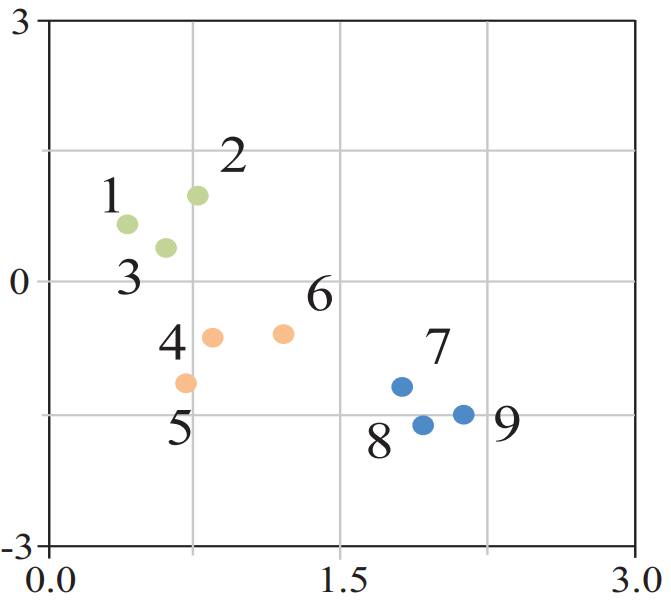
\includegraphics[width=7 cm]{images/graph_emb_2.png}
	\caption{
		Node embedding with each vector representing node features}
	\label{fig:nodeEmbedding}
\end{figure}

Node embedding represents each node as a low-dimensional vector. Nodes that are *close* in the graph have similar vector representations. The difference among graph embedding methods lies in how they define the *closeness* between two nodes. First-order proximity (Definition \ref{def:firstOrderProximity}) and second-order proximity (Definition \ref{def:secondOrderProximity}) are two commonly used metrics to measure pairwise node similarity. Higher-order proximity has also been explored to some extent. For example, capturing k-step (k = 1, 2, 3, ···) neighborhood relationships during embedding is discussed in the study by Cao, Shaosheng \cite{cao2015grarep}.

\textbf{Edge Embedding}
\label{sec:edgeEmbedding}

\begin{figure}[htp]
	\centering
	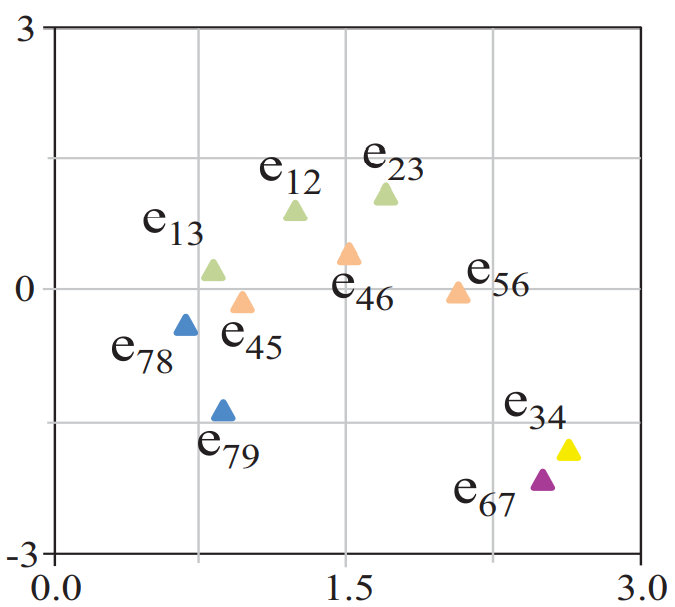
\includegraphics[width=7 cm]{images/graph_emb_3.png}
	\caption{Edge embedding with each vector representing edge features}
	\label{fig:edgeEmbedding}
\end{figure}

In contrast to node embedding, edge embedding aims to represent an edge as a low-dimensional vector. Edge embedding is useful in two cases:

First, in knowledge graph embedding. Each edge is a triple $\langle h, r, t \rangle$ (Definition \ref{def:knowledgeGraph}). The embedding is learned to preserve the relation $r$ between $h$ and $t$ in the embedding space so that a missing entity or relation can be accurately predicted given the other two components in $\langle h, r, t \rangle$.

Second, some methods embed a pair of nodes as a vector to compare it with other node pairs or to predict the existence of a link between the two nodes. Edge embedding benefits graph analyses that involve edges (node pairs), such as link prediction, relation prediction, and knowledge-based entity inference.

\textbf{Hybrid Embedding}

\begin{figure}[htp]
	\centering
	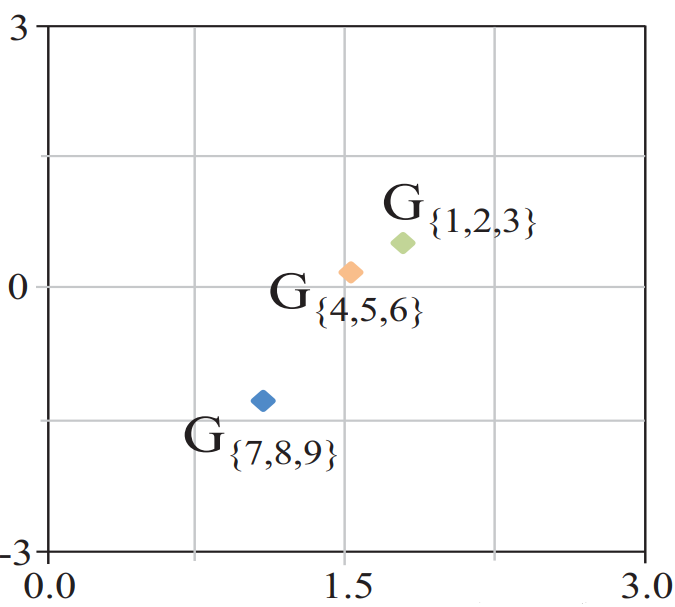
\includegraphics[width=6 cm]{images/graph_emb_4.png}
	\caption{Embedding a graph substructure}
	\label{fig:substructureEmbedding}
\end{figure}

Hybrid embedding refers to embedding combinations of different graph components, e.g., node + edge (i.e., substructure), or node + parts. Substructure or part embeddings can also be derived by aggregating individual node and edge embeddings. However, such *indirect* approaches are not optimized to capture the structure of the graph. Moreover, node and part embeddings can reinforce each other. Node embeddings improve by learning from high-order neighborhood attention, while part embeddings become more accurate due to the collective behavior of their constituent nodes.

\textbf{Whole-Graph Embedding}

\begin{figure}[htp]
	\centering
	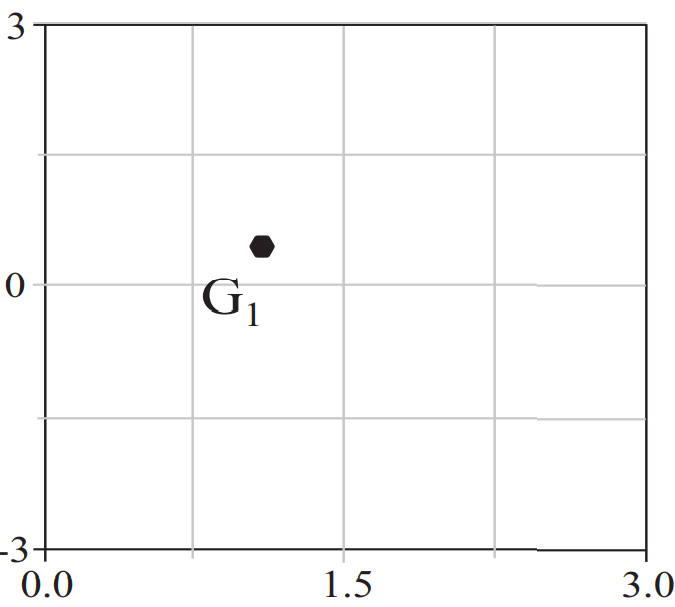
\includegraphics[width=6 cm]{images/graph_emb_5.png}
	\caption{Whole-graph embedding}
	\label{fig:wholeGraphEmbedding}
\end{figure}

Whole-graph embedding is typically used for small graphs such as proteins, molecules, etc. In this case, an entire graph is represented as a vector, and similar graphs are embedded close to each other. Whole-graph embedding is useful for graph classification tasks by providing a simple and effective solution for computing graph similarity. To balance embedding time (efficiency) and information retention (expressiveness), **hierarchical graph embedding** \cite{mousavi2017hierarchical} introduces a hierarchical embedding framework. It argues that accurate understanding of global graph information requires processing substructures at multiple scales. A graph pyramid is formed where each level is a coarsened graph at a different scale. The graph is embedded at all levels and then concatenated into a single vector. Whole-graph embedding requires collecting features from the entire graph, thus is generally more time-consuming than other settings.


\subsection{Graph Embedding Techniques}

\begin{figure}[htp]
	\centering
	\resizebox{\textwidth}{!}{
		\begin{tikzpicture}[
			rec/.style  = {draw, text width=2cm, font=\sffamily, rectangle, thin},
			root/.style = {rec, rounded corners=6pt, align=center, fill=green!60, text width=10em},
			level 1/.style={sibling distance=50mm},
			level 2/.style={rec, rounded corners=6pt, fill=green!30,align=center, text width=8em},
			level 3/.style = {rec, align=left, fill=pink!30, text width=8em, yshift=-20pt},
			edge from parent/.style={->,draw, very thick},
			>=latex]
			
			\node[root] {Graph Embedding Techniques}
			child {node[level 2] (c1) {Deep Learning}}
			child {node[level 2] (c2) {Matrix Factorization}}
			child {node[level 2] (c3) {Edge Reconstruction}}
			child {node[level 2] (c4) {Core Graph}}
			child {node[level 2] (c5) {Generative Models}};
			
			\begin{scope}[every node/.style={level 3}]
				\node [below of = c1, xshift=30pt] (c11) {With random walk};
				\node [below of = c11] (c12) {Without random walk};
				
				\node [below of = c2, xshift=30pt] (c21) {Laplacian Eigenmaps};
				\node [below of = c21] (c22) {Matrix factorization via node approximation};
				
				\node [below of = c3, xshift=25pt] (c31) {Maximizing edge reconstruction probability};
				\node [below of = c31, yshift=-20pt] (c32) {Minimizing distance-based loss};
				\node [below of = c32, yshift=-20pt] (c33) {Minimizing margin-based ranking loss};
				
				\node [below of = c4, xshift=25pt] (c41) {Graphlet-based};
				\node [below of = c41] (c42) {Tree pattern-based};
				\node [below of = c42] (c43) {Random walk-based};
				
				\node [below of = c5, xshift=30pt] (c51) {Latent space-based embedding};
				\node [below of = c51] (c52) {Semantic fusion embedding};
			\end{scope}
			
			\foreach \value in {1,2}
			\draw[->, very thick] (c1.195) |- (c1\value.west);
			
			\foreach \value in {1, 2}
			\draw[->, very thick] (c2.195) |- (c2\value.west);
			
			\foreach \value in {1,...,3}
			\draw[->, very thick] (c3.195) |- (c3\value.west);
			
			\foreach \value in {1,...,3}
			\draw[->, very thick] (c4.195) |- (c4\value.west);
			
			\foreach \value in {1,...,2}
			\draw[->, very thick] (c5.195) |- (c5\value.west);
		\end{tikzpicture}
	}
	\caption{Graph Embedding Techniques}
	\label{fig:graphEmbeddingTechniquesTree}
\end{figure}

In this section, we categorize graph embedding methods based on the techniques used. As previously stated, the goal of graph embedding is to represent a graph in a lower-dimensional space while preserving as much of the original graph information as possible. The main differences among embedding techniques lie in how they define which intrinsic graph properties should be preserved. Since the primary focus of our work is on graph embedding methods based on deep learning, we provide only brief overviews of the other method categories.


\textbf{Deep Learning}

In this section, we present in detail the research directions of deep learning techniques, including: using random walks and not using random walks. Deep learning techniques are widely used in graph embedding due to their speed and efficiency in automatically capturing features. Among these deep learning-based methods, three types of input-based graph settings (excluding graphs constructed from non-relational data) and all four output types (as shown in \autoref{fig:graphEmbeddingSettingTree}) can adopt deep learning approaches.

\textit{Deep learning techniques with random walks}

In this category, the second-order proximity (Definition \ref{def:secondOrderProximity}) in the graph is preserved in the embedding space by maximizing the probability of observing a vertex's neighborhood conditioned on its embedding vector. The graph is represented as a set of samples obtained via random walks, and then deep learning methods are applied to ensure the structural properties (i.e., path-based information) are preserved. Representative methods in this group include: DeepWalk \cite{perozzi2014deepwalk}, LINE \cite{tang2015line}, Node2Vec \cite{grover2016node2vec}, Anonymous Walk \cite{ivanov2018anonymous}, NetGAN \cite{bojchevski2018netgan}, etc.

\textit{Deep learning techniques without random walks}

This approach applies multi-layer learning structures effectively and efficiently to transform the graph into a lower-dimensional space. It operates over the entire graph. Several popular methods have been surveyed and presented in \cite{rossi2020knowledge}, as follows:

\begin{itemize}
	\item \textbf{Convolutional Neural Networks (CNNs)}
	
	This model uses multiple convolutional layers: each layer performs convolution on the input data using low-dimensional filters. The result is a feature map, which then passes through a fully connected layer to compute the probability values. For example, \textbf{ConvE} \cite{dettmers2017convolutional}: each entity and relation is represented as a low-dimensional vector ($d$-dimensional). For each triple, it concatenates and reshapes the head $h$ and relation $r$ embeddings into a single input $[h, r]$ with shape $d_m \times d_n$. This is then passed through a convolutional layer with a filter $\omega$ of size $m \times n$, followed by a fully connected layer with weights $W$. The final result is combined with the tail embedding $t$ using a dot product. This architecture can be considered a \textit{multi-class classification} model.
	
	Another popular model is \textbf{ConvKB} \cite{nguyen2017novel}, which is similar to ConvE but concatenates the three embeddings $h$, $r$, and $t$ into a matrix $[h, r, t]$ of shape $d \times 3$. It is then passed through a convolutional layer with $T$ filters of size $1 \times 3$, resulting in a feature map of size $T \times 3$. This is further passed through a fully connected layer with weights $\mathbf{W}$. This architecture can be considered a binary classification model.
	
	\item \textbf{Recurrent Neural Networks (RNNs)}
	
	These models apply one or more recurrent layers to analyze the entire path (a sequence of events/triples) sampled from the training set, instead of treating each event independently. For example, RSN \cite{guo2019learning} notes that traditional RNNs are unsuitable for graphs because each step only takes the relation information without considering the entity embedding from the previous step. Therefore, it fails to clearly model the transitions among entity-relation paths. To address this, they propose RSN (Recurrent Skipping Networks \cite{guo2019learning}): at each step, if the input is a relation, a hidden state is updated to reuse the entity embedding. The output is then dot-multiplied with the target embedding vector.
	
	\item \textbf{Capsule Neural Networks}
	
	Capsule networks group neurons into "capsules" \label{capsule}, where each capsule encodes specific features of the input, such as representing a particular part of an image. One advantage of capsule networks is their ability to capture spatial relationships that are lost in conventional convolution. Each capsule produces feature vectors. For instance, \textbf{CapsE} \cite{vu2019capsule}: each entity and relation is embedded into vectors, similar to ConvKB. It concatenates the embeddings $h$, $r$, and $t$ into a matrix of shape $d \times 3$, then applies $E$ convolutional filters of size $1 \times 3$, resulting in a $d \times E$ matrix. Each $i$-th row encodes distinct features of $h[i]$, $r[i]$, and $t[i]$. This matrix is then fed into a capsule layer, where each capsule (\ref{capsule}) processes a column, thus receiving feature-specific information from the input triple. A second capsule layer is used to produce the final output.
	
	\item \textbf{Graph Attention Networks (GATs)}
	
	This category uses the attention mechanism \cite{vaswani2017attention}, which has achieved notable success in NLP tasks. For each embedding vector, information from neighboring entities is aggregated using attention weights. These are then combined and passed through a fully connected layer with learnable weights to obtain the final embeddings. For example, GAT \cite{velivckovic2017graph} applies multi-head attention to each training triple to generate an embedding vector. This embedding is then transformed via a weight matrix to produce a higher-dimensional vector that aggregates information from neighboring nodes in the original triple. An improved version, KBGAT \cite{nathani2019learning}, incorporates the relation embedding into the attention mechanism. These methods will be discussed in detail in the subsequent sections.
	
	\item \textbf{Other methods}
	
	There are also other approaches, such as autoencoder-based techniques like Structural Deep Network Embedding (SDNE) \cite{wang2016structural}.
\end{itemize}




\textbf{Matrix Factorization}

Matrix factorization-based graph embedding represents the structural characteristics of a graph (e.g., similarity or proximity between vertex pairs) in the form of a matrix and then factorizes this matrix to obtain vertex embeddings. The input for this category of methods is typically high-dimensional non-relational features, and the output is a set of vertex embeddings. There are two matrix factorization-based graph embedding methods: Graph Laplacian Eigenmaps and Node Proximity Matrix Factorization.

\begin{itemize}
	\item \textit{Graph Laplacian Eigenmaps}
	
	This approach preserves graph properties by analyzing similar vertex pairs and heavily penalizes embeddings that place highly similar nodes far apart in the embedding space.
	
	\item \textit{Node Proximity Matrix Factorization}
	
	This approach approximates neighboring nodes in a low-dimensional space using matrix factorization techniques. The objective is to preserve neighborhood information by minimizing the approximation loss.
\end{itemize}

\textbf{Edge Reconstruction}

The edge reconstruction method builds edges based on the vertex embeddings so that the reconstructed graph is as similar as possible to the input graph. This method either maximizes the edge reconstruction probability or minimizes edge reconstruction loss. Additionally, the loss can be distance-based or margin-based ranking loss.

\begin{itemize}
	\item \textit{Maximize Edge Reconstruction Probability}
	
	In this method, a good vertex embedding maximizes the likelihood of generating observed edges in the graph. In other words, a good vertex embedding should allow for reconstructing the original input graph. This is achieved by maximizing the generative probability of all observed edges using vertex embeddings.
	
	\item \textit{Minimize Distance-Based Loss}
	
	In this approach, embeddings of neighboring nodes should be as close as possible to the observed neighboring nodes in the original graph. Specifically, vertex proximity can be measured using their embeddings or heuristically based on observed edges. The difference between these two types of proximity is then minimized to ensure consistent similarity.
	
	\item \textit{Minimize Margin-Based Ranking Loss}
	
	In this approach, the edges in the input graph represent correlations between vertex pairs. Some vertices in the graph are often linked with related vertex sets. This method ensures that embeddings of related nodes are closer together than unrelated ones by minimizing a margin-based ranking loss.
\end{itemize}

\textbf{Graph Kernels}

Graph kernel methods represent the entire graph structure as a vector containing counts of basic substructures extracted from the graph. Subcategories of graph kernel techniques include: graphlets, subtree patterns, and random walk-based methods.

This approach is designed to embed whole graphs, focusing only on global graph features. The input is typically homogeneous graphs or graphs with auxiliary information.

\textbf{Generative Models}

A generative model is defined by specifying a joint distribution over input features and class labels, parameterized by a set of variables. There are two subcategories of generative model-based methods: embedding graphs into latent space and incorporating semantics for embedding. Generative models can be applied to both node and edge embeddings. They are commonly used to embed semantic information, with inputs often being heterogeneous graphs or graphs with auxiliary attributes.

\begin{itemize}
	\item \textit{Embedding Graphs into Latent Semantic Space}
	
	In this group, vertices are embedded into a latent semantic space where the distance between nodes captures the graph structure.
	
	\item \textit{Incorporating Semantics for Embedding}
	
	In this method, each vertex is associated with graph semantics and should be embedded closer to semantically relevant vertices. These semantic relationships can be derived from descriptive nodes via a generative model.
\end{itemize}

\textbf{Summary}: Each graph embedding method has its own strengths and weaknesses, which have been summarized by Cai, Hongyun \cite{cai2018comprehensive} and are presented in \autoref{tab:graphEmbeddingTechCompare}. The \textit{matrix factorization} group learns embeddings by analyzing pairwise global similarities. The \textit{deep learning} group, in contrast, achieves promising results and is suitable for graph embedding because it can learn complex representations from complex graph structures.

\newcolumntype{L}{>{\arraybackslash}m{0.25\textwidth}}
\newcolumntype{M}{>{\arraybackslash}m{0.2\textwidth}}
\begin{longtable}{|p{0.2\textwidth}|p{0.22\textwidth}|L|p{0.22\textwidth}|}
	\caption{Comparison of Advantages and Disadvantages of Graph Embedding Techniques} \label{tab:graphEmbeddingTechCompare} \\
	\hline
	Method & Subcategory & Advantages & Disadvantages \\
	\hline \hline
	\endfirsthead
	
	%	\multicolumn{4}{c}%
	%	{{\bfseries \tablename\ \thetable{} -- continued from previous page}} \\
	\hline
	Method & Subcategory & Advantages & Disadvantages \\
	\hline \hline
	\endhead
	
	%	\hline \multicolumn{4}{|r|}{{Continued on next page}} \\ \hline
	\endfoot
	
	\hline
	\endlastfoot
	
	Matrix Factorization & Graph Laplacian Eigenmaps & \multirow{3}{=}{Considers global neighborhood structure} &
	\multirow{2}{=}{Requires large computation time and space} \\ \cline{2-2}
	& Node Proximity Matrix Factorization & & \\
	\hline
	\multirow{3}{=}{Edge Reconstruction} & Maximize edge reconstruction probability & \multirow{3}{=}{Relatively efficient training} & \multirow{3}{=}{Only optimizes local information, e.g., first-order neighbors or ranked node pairs} \\ \cline{2-2}
	& Minimize distance-based loss & & \\ \cline{2-2}
	& Minimize margin-based ranking loss & & \\ \hline
	\multirow{3}{=}{Graph Kernels} & Based on graphlet & \multirow{3}{=}{Efficient, considers only desired primitive structures} & \multirow{3}{=}{Substructures are not independent. Embedding dimensionality increases exponentially} \\ \cline{2-2}
	& Based on subtree patterns & & \\ \cline{2-2}
	& Based on random walk & & \\ \hline
	
	Generative Model & Embedding into latent space & Embedding is interpretable & Difficult to tune distribution selection \\ \cline{2-3}
	
	& Incorporate semantics & Leverages multiple information sources & Requires a large amount of naturally labeled data\\
	\hline
	
	Deep Learning & With random walk & \multirow{2}{=}{Efficient and fast. No need for manual feature extraction} & Considers only local path content. Difficult to find optimal sampling strategy \\ \cline{2-2} \cline{4-4} 
	& Without random walk & & High computational cost \\ \hline
\end{longtable}




%\newcolumntype{L}{>{\arraybackslash}m{5cm}}
%\begin{table}[htbp]
%	\begin{center}
%		\caption{Bảng so sánh ưu và nhược điểm của kỹ thuật nhúng đồ thị}
%		\label{tab:graphEmbeddingTechCompare2}
%		\resizebox{\textwidth}{!}{
%			\begin{tabular}{|p{2cm}|p{8cm}|L|p{8cm}|}
%				\hline
%				Phương pháp & Danh mục con & Ưu điểm & Nhược điểm \\
%				\hline \hline
%				Phân rã ma trận & Đồ thị toán tử Laplace Eigenmap & \multirow{3}{5cm}{Xem xét toàn cục các đỉnh lân cận}&
%				\multirow{2}{8cm}{Sử dụng không gian và thời gian tính toán lớn }\\
%				\cline{2-2}
%				& Phân rã ma trận bằng xấp xỉ đỉnh & & \\
%				\hline
%				\multirow{3}{2cm}{Tái cấu trúc cạnh} & Cực đại hóa xác suất tái cấu trúc cạnh & \multirow{3}{5cm}{Huấn luyện tương đối hiệu quả} & \multirow{3}{8cm}{Tối ưu chỉ sử dụng thông tin cục bộ. Ví dụ như các cạnh (hàng xóm 1 nước) hoặc cặp đỉnh xếp hạng } \\ \cline{2-2}
%				& Tối thiểu hóa mất mát dựa trên khoảng cách & & \\ \cline{2-2}
%				& Tối thiểu hóa xếp hạng mất mát dựa trên lề & & \\ \hline
%				\multirow{3}{2cm}{Đồ thị lõi} & Dựa trên graphlet & \multirow{3}{5cm}{Hiệu quả, chỉ tính những nhánh cấu trúc đơn vị mong muốn} & \multirow{3}{8cm}{Nhánh cấu trúc thì không độc lập. Số chiều nhúng tăng lên theo hàm mũ} \\ \cline{2-2}
%				& Dựa trên mẫu nhánh cây   & & \\ \cline{2-2}
%				& Dựa trên bước nhảy ngẫu nhiên & & \\ \hline
%				
%				Mô hình sinh & Nhúng đồ thị dựa trên không gian ẩn & Phép nhúng có thể giải thích được & Khó điều chỉnh lựa chọn phân bố \\ \cline{2-3}
%				
%				& Nhúng kết hợp ngữ nghĩa & Tận dụng nhiều thông tin nguồn & Yêu cầu một lượng lớn dữ liệu huấn luyện một cách tự nhiên\\
%				\hline
%				
%				Học sâu & Sử dụng bước ngẫu nhiên & \multirow{2}{5cm}{Hiệu quả và nhanh chóng Không phải trích đặc trưng} & Chỉ xem xét đến nội dung cục bộ trong một đường đi. Khó để tìm kiếm chiến lược lấy mẫu tối ưu \\ \cline{2-2} \cline{4-4} 
%				& Không sử dụng bước ngẫu nhiên &  & Chi phí tính toán cao \\ \hline
%			\end{tabular}
%		}
%	\end{center}
%\end{table}
	

Graph embedding methods based on random walk in deep learning have lower computational cost compared to those using full deep learning models. Traditional methods often treat graphs as grids; however, this does not reflect the true nature of graphs. In the \textit{edge reconstruction} group, the objective function is optimized based on observed edges or by ranking triplets. While this approach is more efficient, the resulting embedding vectors do not account for the global structure of the graph. The \textit{graph kernel} methods transform graphs into vectors, enabling graph-level tasks such as graph classification. Therefore, they are only effective when the desired primitive structures in a graph can be enumerated. The \textit{generative model} group naturally integrates information from multiple sources into a unified model. Embedding a graph into a latent semantic space produces interpretable embedding vectors using semantics. However, assuming the modeling of observations using specific distributions can be difficult to justify. Moreover, generative approaches require a large amount of training data to estimate a model that fits the data well. Hence, they may perform poorly on small graphs or when only a few graphs are available.

Among these methods, deep learning-based graph embedding allows learning complex representations and has shown the most promising results. Graph attention networks (GATs), which are based on attention mechanisms, aggregate the information of an entity using attention weights from its neighbors relative to the central entity. We believe this research direction is aligned with studies on the relationship between attention and memory \cite{memoryandattention:2020}, where the distribution of attention determines the weight or importance of one entity relative to another. Likewise, the embedding vector representing an entity is influenced by the attention or importance of its neighboring embeddings. Therefore, this is the approach we selected among the existing graph embedding methods.

\section{Multi-head Attention Mechanism}

In 2014, the multi-head attention mechanism was introduced by Bahdanau, Dzmitry \cite{bahdanau2014neural}, but it only gained widespread popularity in 2017 through the Transformer model by Vaswani, Ashish \cite{vaswani2017attention}. The attention mechanism is an effective method to indicate the importance of a word with respect to other words in a sentence, and it has been shown to be a generalization of any convolution operation as reported by Cordonnier, Jean-Baptiste \cite{cordonnier2019relationship}. To understand how multi-head attention is applied to graphs, in this section we will detail the mechanism so we can better understand how it is used in link prediction tasks within knowledge graphs.

\subsection{Attention Mechanism}
\label{sec:attentionMechanism}

The input of the attention mechanism consists of two embedding matrices $\mathbf{X} = \Big\{\overrightarrow{x_1}, \overrightarrow{x_2}, ...,  \overrightarrow{x_{N_x}}\Big\}$ and $\mathbf{Y} = \Big\{\overrightarrow{y_1}, \overrightarrow{y_2}, ...,  \overrightarrow{y_{N_y}}\Big\}$, where each row $i^{\text{th}}$ or $j^{\text{th}}$ in matrix $\mathbf{X}$ or $\mathbf{Y}$ is an embedding vector $\overrightarrow{x_i} \in \mathbb{R}^{1 \times D_{\text{in}}}$, $\overrightarrow{y_j} \in \mathbb{R}^{1 \times D_{\text{in}}}$.

The attention mechanism transforms input vectors of $D_{\text{in}}$ dimensions into output vectors of $D_{\text{attention}}$ dimensions to represent the importance of each of the $N_x$ elements $x$ with respect to all $N_y$ elements $y$. Given $\mathbf{X} \in \mathbb{R}^{N_x \times D_\text{in}}$ and $\mathbf{Y} \in \mathbb{R}^{N_y \times D_\text{in}}$ as input embedding matrices, and $\mathbf{H} \in \mathbb{R}^{N_x \times D_\text{attention}}$ as the output embedding matrix, the attention mechanism introduced by Vaswani et al. \cite{vaswani2017attention} is defined as follows:

\begin{equation}
	\label{attention}
	\mathbf{H} = \text{Attention}(\mathbf{Q}, \mathbf{K}, \mathbf{V}) = \text{softmax}\Big(\frac{\mathbf{Q}\mathbf{K}^T}{\sqrt{d_k}}\Big) \mathbf{V}
\end{equation}

where $\mathbf{Q} = \mathbf{X}\mathbf{W}_Q, \mathbf{K} = \mathbf{Y} \mathbf{W}_K, \mathbf{V} = \mathbf{Y} \mathbf{W}_V$.

The weight matrices 
$\mathbf{W}_Q \in \mathbb{R}^{D_{\text{in}} \times D_{k}}$, 
$\mathbf{W}_K \in \mathbb{R}^{D_{\text{in}} \times D_{k}}$, and 
$\mathbf{W}_V \in \mathbb{R}^{D_{\text{in}} \times D_{\text{attention}}}$ 
are used to parameterize the transformation from input embedding vectors of dimension $D_{\text{in}}$ into output embedding vectors of dimension $D_k$ or $D_{\text{attention}}$. The term $\mathbf{Q}\mathbf{K}^T$ represents the dot product between each vector $x$ and all vectors $y$. Dividing by $\sqrt{d_k}$ normalizes the result with respect to the vector dimension $k$. The result is then passed through the \textit{softmax} function to enable comparison of attention scores across different pairs. We can interpret $\text{softmax}\Big(\frac{\mathbf{Q}\mathbf{K}^T}{\sqrt{d_k}}\Big)$ as the \textit{attention coefficients}, indicating the importance of each $y$ with respect to each $x$. Finally, this is multiplied with the value matrix $\mathbf{V}$ to produce the final output embedding of dimension $D_{\text{attention}}$.

If $\mathbf{X} = \mathbf{Y}$, we are computing the importance of each element with respect to other elements in the same input matrix, which is referred to as the self-attention mechanism.


\subsection{Multi-Head Attention}

The multi-head attention mechanism is a way of combining multiple attention layers to stabilize the learning process. Similar to the standard attention mechanism above, the multi-head attention mechanism transforms the initial $N_x$ embedding vectors of dimension $D_{\text{in}}$ into output embedding vectors of dimension $D_{\text{multi-head}}$, aggregating information from various other nodes to provide greater stability during training. Multi-head attention stacks $N_{\text{head}}$ attention output matrices $\mathbf{H}$, and then applies a weight matrix to transform the original embedding matrix $\mathbf{X} \in \mathbb{R}^{N_x \times D_\text{in}}$ into a new embedding matrix $\mathbf{X}' \in \mathbb{R}^{N_x \times D_{\text{multi-head}}}$ using the following formula:

\begin{equation}
	\label{headAttention}
	\begin{split}
		\mathbf{X}'& =\left(\bigparallel_{h=1}^{N_{\text{head}}}\mathbf{H}^{(h)}\right)\mathbf{W}^{O} \\
		& = \left(\bigparallel_{h=1}^{N_{\text{head}}} \text{Attention}(\mathbf{X} \mathbf{W}_Q^{(h)}, \mathbf{Y} \mathbf{W}_K^{(h)}, \mathbf{Y} \mathbf{W}_V^{(h)}) \right)\mathbf{W}^{O}
	\end{split}
\end{equation}

Here, the weight matrices $\mathbf{W}_Q^{(h)}$, $\mathbf{W}_K^{(h)} \in \mathbb{R}^{D_{\text{in}} \times D_{k}}$, and $\mathbf{W}_V^{(h)} \in \mathbb{R}^{D_{\text{in}} \times D_{\text{attention}}}$ correspond to each individual attention head $h \in [N_{\text{head}}]$. The output projection matrix $\mathbf{W}^{O} \in \mathbb{R}^{N_{\text{head}} D_{\text{attention}} \times D_{\text{multi-head}}}$ parameterizes the transformation of the concatenated output heads into the final output embedding matrix.

At this point, we have presented the attention mechanism for computing attention scores and aggregating embedding information from neighboring vectors. In the next section, we will describe how this attention mechanism is applied to knowledge graphs.

%\textbf{Lớp cộng tác đa đỉnh chú ý}

%\cite{weng2018attention}

\section{Graph Attention Network}
\label{sec:GAT}

\begin{figure}[htp]
	\centering
	% (TikZ content unchanged)
	\caption{Knowledge graph and normalized attention coefficients of the entity}
	\label{fig:graphExample}
\end{figure}

With the success of the \textit{multi-head attention mechanism} in natural language processing, it has also been studied for applications in image processing models \cite{ramachandran2019stand}. Consequently, the multi-head attention mechanism has been explored for replacing convolutional operations in knowledge graph embedding models, such as Graph Convolutional Networks (GCNs \cite{kipf2016semi}). In this section, we present in detail how the attention mechanism from \ref{sec:attentionMechanism} is applied to graph embedding via the Graph Attention Network (GAT \cite{velivckovic2017graph}) method.

The input to the \textit{graph attention network} model is a set of embedding vectors, randomly initialized from a normal distribution, representing features of each entity: $\mathbf{E} = \Big\{\overrightarrow{e_1}, \overrightarrow{e_2}, ...,  \overrightarrow{e_{N_e}}\Big\}$. The objective of the model is to transform this into a new output embedding matrix $\mathbf{E}'' = \Big\{\overrightarrow{e''_1}, \overrightarrow{e''_2}, ...,  \overrightarrow{e''_{N_e}}\Big\}$ capable of aggregating embedding information from neighboring entities. Here, $\mathbf{E} \in \mathbb{R}^{N_e \times D_{\text{in}}}$ and $\mathbf{E}'' \in \mathbb{R}^{N_e \times D''}$ denote the input and output embedding matrices for the entity set, respectively. $N_e$ is the number of entities, and $D_{\text{in}}$, $D''$ are the dimensions of the input and output embeddings.

Similar to the multi-head attention mechanism introduced in \ref{sec:attentionMechanism}, the application of this mechanism to a knowledge graph follows the same logic as the \textit{self-attention mechanism}, in which each node attends to all other nodes in the graph. However, computing attention scores between every pair of nodes in a graph is not meaningful if no relationship exists between them, and it would incur significant computational overhead. Therefore, the model applies a technique known as \textit{masked attention}, in which all attention scores corresponding to unrelated nodes in the graph are ignored. These relevant connections are precisely defined as the first-order proximity (Definition \ref{def:firstOrderProximity}) of a node in the graph. Thus, in this context, we let $\mathbf{X} = \mathbf{Y} = \mathbf{E}$ (as in \ref{sec:attentionMechanism}), and the attention coefficient in the masked attention mechanism represents the importance of a neighboring node $j \in \mathcal{N}_{i}$ to the central node $i$, where $\mathcal{N}_{i}$ is the set of all first-order neighbors of node $i$ (including $i$ itself).




The application of the multi-head attention mechanism (\textit{multi-head attention}) in \ref{headAttention} to graphs is described as follows:

\begin{equation}
	\label{maskAttention}
	\centering
	{e_{ij}}={f_{\text{mask attention}}(\mathbf{W} \overrightarrow{e_i}, \mathbf{W} \overrightarrow{e_j})}
\end{equation}

where $e_{ij}$ denotes the multi-head attention coefficient of an edge $(e_i, e_j)$ with respect to the central entity $e_i$ in the knowledge graph $\mathcal{G}_{\text{know}}$. $\mathbf{W}$ is a weight matrix that parameterizes the linear transformation. $f_{\text{mask attention}}$ is the function applying the attention mechanism.

In the GAT model, each entity vector embedding $\overrightarrow{e_i}$ undergoes two transformation stages. The entire model consists of two transformation steps, each applying the multi-head attention mechanism as follows:

\begin{equation}
	\label{gatProcess}
	\overrightarrow{e_i} \xrightarrow{f_{\text{mask attention}}^{(1)}} \overrightarrow{e'_i} \xrightarrow{f_{\text{mask attention}}^{(2)}} \overrightarrow{e''_i}
\end{equation}

In the first multi-head attention step ($f_{\text{mask attention}}^{(1)}$), the model aggregates information from neighboring entities and stacks them to produce vector $\overrightarrow{e'_i}$, where $\overrightarrow{e'_i} \in \mathbb{R}^{1 \times D'}$. In the second step ($f_{\text{mask attention}}^{(2)}$), the multi-head attention layer is no longer sensitive to self-attention; therefore, the output is computed as an \textit{average} instead of concatenating attention heads. The vector $\overrightarrow{e'_i}$ is then treated as the input embedding to be transformed into the final output embedding vector $\overrightarrow{e''_i}$, with $\overrightarrow{e''_i} \in \mathbb{R}^{1 \times D''}$.

First, similar to the attention mechanism in \ref{attention}, each embedding vector is multiplied by a weight matrix $\mathbf{W}_1 \in \mathbb{R}^{D_k \times D_{\text{in}}}$ to parameterize the linear transformation from $D_{\text{in}}$ input dimensions to $D_k$ higher-level feature dimensions:

\begin{equation}
	\overrightarrow{h_i} = \mathbf{W}_{1} \overrightarrow{e_i}
\end{equation}

where $\overrightarrow{e_i} \in \mathbb{R}^{D_{\text{in}} \times 1}
\xrightarrow{} \overrightarrow{h_i} \in \mathbb{R}^{D_k \times 1}$


Next, we concatenate each pair of linearly transformed entity embedding vectors to compute the attention coefficients. The attention coefficient $e_{ij}$ reflects the importance of the edge feature $(e_i, e_j)$ with respect to the central entity $e_i$, or in other words, the importance of a neighboring entity $e_j$ that is connected to $e_i$. We apply the $\text{LeakyReLU}$ function to extract the absolute value of the attention coefficient. Each attention coefficient $e_{ij}$ is computed using the following equation:

\begin{equation}
	e_{ij} = \Big( \text{LeakyReLU} \Big( \overrightarrow{\mathbf{W}_{2}}^{T} [\overrightarrow{h_i} || \overrightarrow{h_j}]\Big) \Big)
\end{equation}

where ${.}^{T}$ denotes the transpose operation and $||$ represents concatenation. This is similar to \ref{attention}, however instead of using a dot product, we use a \textit{shared attentional mechanism} $\overrightarrow{\mathbf{W}_2}$: $\mathbb{R}^{D_k} \times \mathbb{R}^{D_k} \rightarrow \mathbb{R}$ to compute the attention scores. As mentioned in \ref{maskAttention}, we perform self-attention between all nodes using the masked attention mechanism to discard all irrelevant structural information.

To enable meaningful comparison between the attention coefficients of neighboring entities, a \textit{softmax} function is applied to normalize the coefficients over all neighbors $e_j$ that are connected to the central entity $e_i$: $\alpha_{ij} = \text{softmax}_j(e_{ij})$. Combining all of this, we obtain the final normalized attention coefficient of each neighbor with respect to the central entity as follows:

\begin{equation}
	\label{attentionCoeff}
	\alpha_{ij} = \frac{
		\text{exp} \Big( \text{LeakyReLU} \Big( \overrightarrow{\mathbf{W}_2}^{T} [ \overrightarrow{h_i} || \overrightarrow{h_j}]\Big) \Big))
	}
	{
		\sum_{k \in \mathcal{N}_i}
		\text{exp} \Big( \text{LeakyReLU} \Big( \overrightarrow{\mathbf{W}_2}^{T} [\overrightarrow{h_i} || \overrightarrow{h_k}]\Big) \Big))
	}
\end{equation}





At this stage, the GAT model operates similarly to GCN \cite{kipf2016semi}, where the embedding vectors from neighboring nodes are aggregated and scaled by their corresponding normalized attention coefficients:

\begin{equation}
	\label{scaleAttentionCoef}
	\centering
	{\overrightarrow{e'_i}}={\sigma\left(\sum_{j\in \mathcal{N}_i} {\alpha_{ij} \overrightarrow{h_j} }\right)}
\end{equation}

Similar to the multi-head attention layer, we concatenate $N_{\text{head}}$ attention heads to stabilize the training process in the first step ($f_{\text{mask attention}}^{(1)}$ \ref{gatProcess}) of the model:

\begin{equation}
	\label{multiHeadAttention}
	{\overrightarrow{e'_i}}={\bigparallel_{h=1}^{N_{\text{head}}}\sigma\left(\sum_{j\in \mathcal{N}_i}\alpha_{ij}^{h} \mathbf{W}^{h} \overrightarrow{h_{j}} \right)}
\end{equation}

where $\sigma$ is any non-linear activation function, and $\alpha_{ij}^h$ is the normalized attention coefficient for edge $(e_i, e_j)$ computed from the $h^{th}$ attention head. Similar to equation \ref{attention}, $\mathbf{W}^h$ is the weight matrix used for linear transformation of the input embedding vector, with each $\mathbf{W}^h$ corresponding to a different attention head. The resulting new embedding vector $\overrightarrow{e'_i} \in \mathbb{R}^{1 \times D'}$, where $D' = N_{\text{head}} D_{\text{k}}$, is then used as the input for the next attention layer. However, in the second step ($f_{\text{mask attention}}^{(2)}$ \ref{gatProcess}), the multi-head attention outputs are averaged instead of concatenated, as shown below:

\begin{equation}
	\label{multiHeadConcat}
	{\overrightarrow{e''_i}}={\sigma\left(\frac{1}{N_{\text{head}}} \sum_{h=1}^{N_{\text{head}}}\sum_{j\in \mathcal{N}_i}\alpha_{ij}^{h} \mathbf{W}^{h} \overrightarrow{e'_{j}} \right)}
\end{equation}



\textbf{Summary}: Up to this point, we have presented how the attention mechanism aggregates a knowledge graph entity embedding vector from its neighboring embeddings and concatenates them to produce the final embedding. In the next section, we will present our complete embedding model based on the KBGAT model proposed by Nathani, Deepak\cite{nathani2019learning}.

\section{KBGAT Model}

In a knowledge graph, a single entity cannot fully represent an edge, as the entity can play multiple roles depending on the type of relation. For example, in \autoref{fig:graphExample}, Donald Trump serves both as a president and as a husband. To address this issue, the knowledge graph attention-based embedding model — KBGAT (graph attention based embeddings \cite{nathani2019learning}) — improves upon the GAT model by incorporating additional information from \textit{relations and neighboring node features} into the attention mechanism. In this section, we will detail the KBGAT model. The structure of KBGAT follows an encoder-decoder framework, where the encoder is implemented using the Graph Attention Network (GAT), and the decoder uses the ConvKB model for prediction. The steps of the KBGAT model are illustrated in \ref{eq:KBGATProcess}.

\begin{equation}
	\label{eq:KBGATProcess}
	entities \xrightarrow{\text{Embedding}^{\ref{sec:initTransE}}} \overrightarrow{e_{\text{TransE}}} \xrightarrow{\text{Embedding} ^{\ref{sec:encodeKBGAT}}} \overrightarrow{e_{\text{KBGAT}}} \xrightarrow{\text{ConvKB}^{\ref{sec:predictionConvKB}}} e_{\text{prob}}
\end{equation}

First, the embedding vectors of each entity are initialized using the TransE model to capture the spatial characteristics among nodes and obtain the initial embeddings. These embeddings are then further trained using an encoder model to capture neighborhood features, resulting in updated embeddings. Finally, these embeddings are passed through a prediction layer using the ConvKB model. All equations presented here are based on those in the work of Nathani, Deepak\cite{nathani2019learning}.




\subsection{Embedding Initialization}
\label{sec:initTransE}

\begin{figure}[htp]
	\centering
	\begin{tikzpicture}[
		arrow/.style={->,thick},
		vector/.style={arrow, ultra thick},
		dashLine/.style={->, thin, dash pattern=on 1mm off 0.5mm},
		formal/.style={font=\sffamily}]
		\coordinate (root) at (0,0);
		\coordinate [formal, label=above left:$\overrightarrow{\text{relation}}$] (c1) at (-1.5, 3);
		\coordinate [formal, label=above:$\overrightarrow{\text{tail}_{\text{invalid}}}$] (c2) at (3.5, 5);
		\coordinate [formal, label=right:$\overrightarrow{\text{tail}_{\text{valid}}}$] (c3) at (3.5, 4);
		\coordinate [formal, label=above right :$\overrightarrow{\text{head}_{\text{invalid}}}$] (c4) at (5, 2);
		\coordinate [formal, label=right:$\overrightarrow{\text{head}_{\text{valid}}}$] (c5) at (5, 1);
		
		\draw [arrow] ([yshift=-2em] root) -> (0, 5) node (yaxis)[above] {$y$};
		\draw [arrow] ([xshift=-5em] root) -> (5, 0) node (xaxis)[above] {$x$};
		
		\foreach \x in {3, 5}
		{\draw [vector, color=azure] (root) -> (c\x);}
		
		\foreach \x in {2, 4}
		{\draw [vector, color=awesome] (root) -> (c\x);}
		
		\draw [vector, color=amber] (root) -> (c1);
		
		\foreach \x in {1, 4}
		{\draw [dashLine, color=darkpastelgreen] (c\x) -> (c2);}
		
		\foreach \x in {1, 5}
		{\draw [dashLine, color=darkpastelgreen] (c\x) -> (c3);}
	\end{tikzpicture}
	\caption{Illustration of embedding vectors in the TransE model}
	\label{fig:TransEAnimation}
\end{figure}

Similar to the Word2Vec method \cite{mikolov2013efficient}, the model \textit{Translating Embeddings for Modeling Multi-relational Data} (TransE \cite{bordes2013translating}) belongs to the group of geometric embedding methods that transform entities and relations in a knowledge graph into output embedding vectors such that:
\begin{equation}
	\label{eq:conditionTransE}
	\overrightarrow{\text{entity}_{\text{head}}} + \overrightarrow{relation} \approx \overrightarrow{\text{entity}_{\text{tail}}}
\end{equation}

Initially, the entity and relation embedding vectors are randomly initialized using a normal distribution with dimensionality $D_{\text{in}}$, and then normalized according to the size of the entity and relation embedding sets.


Next, we perform sampling from the training dataset to obtain a batch of valid triples ($S_{\text{batch}}$). For each such triple, we sample an invalid triple by replacing either the head or the tail entity with a random entity from the entity set, yielding a batch of invalid triples ($S'_{\text{batch}}$). We then pair each valid triple with an invalid one to form the training batch ($T_{\text{batch}}$). Finally, we update the embedding vectors to satisfy the condition in \ref{eq:conditionTransE}.

\begin{algorithm}
	\caption{TransE Embedding Learning Algorithm \protect\cite{bordes2013translating}}\label{alg:TransE}
	\begin{algorithmic}[1]
		\Statex \textbf{Input} :
		Training set $S = {(h, r, t)}$, entity set $E$, relation set $R$, margin $\gamma$, embedding dimension $D_{\text{in}}$	
		\Statex \textbf{Initialize}
		\State $\overrightarrow{r} \leftarrow \text{uniform}(-\frac{6}{\sqrt{D_{\text{in}}}}, \frac{6}{\sqrt{D_{\text{in}}}})$ for each relation $r \in R$
		\State $\overrightarrow{r} \leftarrow \frac{\overrightarrow{r}}{\|\overrightarrow{r}\|}$ for each $r \in R$
		\State $\overrightarrow{e} \leftarrow \text{uniform}(-\frac{6}{\sqrt{D_{\text{in}}}}, \frac{6}{\sqrt{D_{\text{in}}}})$ for each entity $e \in E$
		\Loop
		\State $\overrightarrow{e} \leftarrow \frac{\overrightarrow{e}}{\|\overrightarrow{e}\|}$ for each $e \in E$
		\State $S_{\text{batch}} \leftarrow \text{sample}(S, b)$  // sample minibatch of size $b$
		\State $T_{\text{batch}} \leftarrow \varnothing $
		\For {$(h, r, t) \in S_{\text{batch}}$}
		\State $(h', r, t') \leftarrow \text{sample}(S'_{(h, r, t)})$ // sample from invalid triple set
		\State $T_{\text{batch}} \leftarrow T_{\text{batch}} \cup \Big\{ \Big( (h, r, t), (h', r, t') \Big) \Big\}$
		\EndFor
		\Statex Update embeddings
		\State $\sum_{\Big( (h, r, t), (h', r, t')\Big) \in T_{\text{batch}}} \nabla [\gamma + d(\overrightarrow{h} + \overrightarrow{r}, \overrightarrow{t}) - d(\overrightarrow{h'} + \overrightarrow{r}, \overrightarrow{t'})]_{+}$
		\EndLoop
		\Statex \textbf{Output} :
		A set of embedding vectors with dimension $D_{\text{in}}$ representing entities and relations
	\end{algorithmic}
\end{algorithm}

The TransE model proposed by Bordes, Antoine \cite{bordes2013translating} is presented in Algorithm \ref{alg:TransE}.


The input of the TransE model is a training dataset where each element is a triple $(h, r, t)$. Here, $h, t \in E$ are the head and tail entities, and $r \in R$ is the relation. $\overrightarrow{e}$ and $\overrightarrow{r}$ are the embedding vectors of entities and relations respectively, and $\|\overrightarrow{e}\|$ and $\|\overrightarrow{r}\|$ denote the cardinalities of the entity and relation sets. $S$ and $S_{\text{batch}}$ represent the full training dataset and a sampled batch from it, respectively. $T_{\text{batch}}$ is a batch containing both valid and invalid triples used to compute the loss function \ref{eq:sampleTransE}.

A \textit{valid triple} is one directly sampled from the training set ($S_{\text{batch}}$), while an \textit{invalid triple} is constructed by corrupting a valid triple ($S'_{\text{batch}}$) by replacing either the head or the tail entity with a randomly selected entity from the entity set:

\begin{equation}
	\label{eq:sampleTransE}
	\centering
	S'_{(h, r, t)} = \big\{ (h', r, t) | h' \in E \big\} \cup \big\{ (h, r, t') | t' \in E \big\}
\end{equation}

To achieve the goal of learning embedding vectors such that $\overrightarrow{h} + \overrightarrow{r} \approx \overrightarrow{t}$, the model aims for the tail embedding $\overrightarrow{t}$ of valid triples to lie close to $\overrightarrow{h} + \overrightarrow{r}$, while in invalid triples, the corrupted embedding $\overrightarrow{h'} + \overrightarrow{r}$ (or $\overrightarrow{t'}$) should lie far from $\overrightarrow{t}$ (or $\overrightarrow{h} + \overrightarrow{r}$), according to the following margin-based ranking loss function:

\begin{equation}
	\label{eq:KBGATLoss}
	\centering
	\mathcal{L} = \sum_{(h, r, t) \in S} \sum_{(h', r, t') \in S'_{(h, r, t)}} [d - d' + \gamma]_{+}
\end{equation}


% \begin{figure}[htp]
	% 	\centering
	% 	\begin{tikzpicture}[
		% 		arrow/.style={->,thick},
		% 		vector/.style={arrow, ultra thick},
		% 		mapping/.style={->, thin},
		% 		distArrow/.style={thin, <->},
		% 		dashLine/.style={very thin, dash pattern=on 1mm off 0.5mm},
		% 		formal/.style={font=\sffamily}]
		
		% 		\coordinate (root) at (0,0);
		% 		\coordinate [formal, label=above left:$\overrightarrow{h'}$] (c1) at (-1.5, 3);
		% 		\coordinate [formal, label=above:$\overrightarrow{t}$] (c2) at (2, 5);
		% 		\coordinate [formal, label=above:$\overrightarrow{t'}$] (c3) at (3.2, 4.5);
		% 		\coordinate [formal, label=above right :$\overrightarrow{h'} + \overrightarrow{r}$] (c4) at (4.5, 4);
		% 		\coordinate [formal, label=right:$\overrightarrow{r}$] (c5) at (6, 1);
		
		% 		\draw [arrow] ([yshift=-1.5em] root) -> (0, 5) node (yaxis)[above] {$y$};
		% 		\draw [arrow] ([xshift=-5em] root) -> (7, 0) node (xaxis)[above] {$x$};
		
		% 		\foreach \x in {1, 5}
		% 		{\draw [vector, color=black] (root) -> (c1);}
		% 		{\draw [vector, color=black] (root) -> (c2);}
		% 		{\draw [vector, color=awesome] (root) -> (c3);}
		% 		{\draw [vector, color=azure] (root) -> (c4);}
		% 		{\draw [vector, color=black] (root) -> (c5);}
		
		% 		\draw [dashLine] (c2) -> (2, -1.5) node (mapc2){};
		% 		\draw [dashLine] (c4) -> (4.5, -1.5) node (mapc4){};
		
		% 		\draw [dashLine, color=amber] (c3) -> (3.2, -0.7) node (mapc3){};
		% 		\draw [dashLine, color=amber] (c4) -> (4.5, -0.7) node (mapc4){};
		
		% 		\draw [distArrow] (2, -1.5) node (map1c2) {} -> (3.5, -1.5) node (alpha)[yshift=2mm] {$\Delta$} -> (4.5, -1.5) node (mapc4){};
		% 		\draw [distArrow] (3.2, -0.7) node (map1c3) {} -> (4, -0.7) node (alpha)[yshift=2mm] {$\Delta'$} ->  (4.5, -0.7) node (mapc4){};
		% 	\end{tikzpicture}
	% 	\caption{Minh học về độ đo hàm loss trong TransE}
	% 	
	% \end{figure}
	
	
\begin{figure}[htp]
	\centering
	\resizebox{\textwidth}{!}{%
		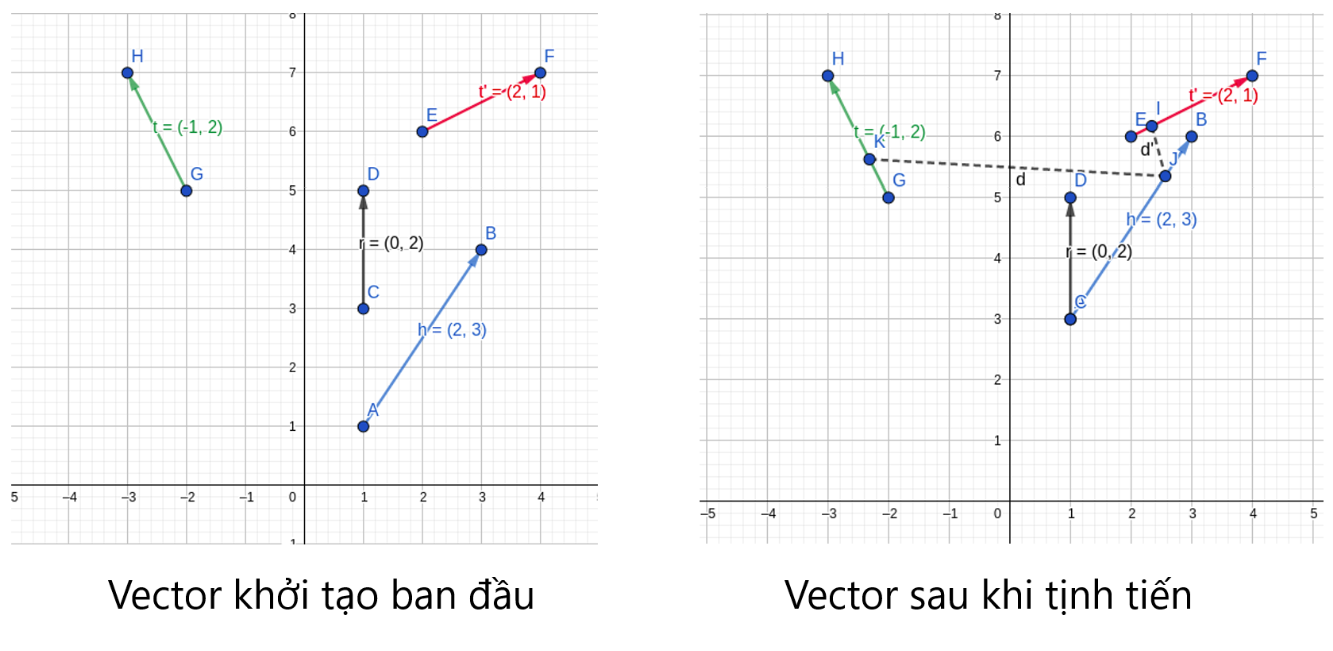
\includegraphics{images/transe.png}
	}
	\caption{TransE embedding model}
	\label{fig:TransEExplain}
\end{figure}

Here, $\gamma > 0$ is the margin, and $h'$ and $t'$ are entities sampled as defined in Equation \ref{eq:sampleTransE}. $\Delta$ and $\Delta'$ represent the difference vectors for the embeddings in valid and invalid triples, respectively, with $d = \big\|\Delta \big\|_{1} = \big\| \overrightarrow{h} + \overrightarrow{r} - \overrightarrow{t} \big\|_{1}$ and $d' = \big\|\Delta' \big\|_{1} = \big\| \overrightarrow{h'} + \overrightarrow{r} - \overrightarrow{t'} \big\|_{1}$, where $\|\cdot\|_{1}$ denotes the L1 norm.

As illustrated in \autoref{fig:TransEExplain}, if $d > d'$ or $d - d' > 0$, then $\overrightarrow{h} + \overrightarrow{r}$ is closer to $\overrightarrow{t}$ than to $\overrightarrow{t'}$. Since we want the embedding vectors to satisfy the condition in Equation \ref{eq:conditionTransE}, $\overrightarrow{h} + \overrightarrow{r}$ should be as close as possible to $\overrightarrow{t}$. That means, the closer $\overrightarrow{h} + \overrightarrow{r}$ is to $\overrightarrow{t'}$, the more incorrect it becomes.

Therefore, during training, we aim for $\Delta'$ to be as large as possible relative to $\Delta$. If $\Delta' > \Delta$ or $d' - d > 0$, there is no need to update the embedding weights further. Hence, in the loss function \ref{eq:KBGATLoss}, the term $[d - d' + \gamma]_{+}$ captures only the positive part because the negative part already satisfies the correctness of the condition in Equation \ref{eq:conditionTransE} during training.



\subsection{Encoder Model}
\label{sec:encodeKBGAT}

After obtaining the embedding vectors that capture spatial features of the knowledge graph, these embeddings are passed through the next embedding layer to further aggregate the neighborhood information of each entity.


\begin{figure}[htp]
	\centering
	\resizebox{\textwidth}{!}{%
		\begin{tikzpicture}[
			emb/.style={draw, circle,minimum width=.1em, thin, anchor=center},
			entityInit/.style={emb, fill=amber},
			relationInit/.style={emb, fill=azure},
			entityEmb/.style={emb, fill=gray},
			relationEmb/.style={emb, fill=deepcarminepink},
			entityPretrain/.style={emb, fill=deepmagenta},
			entityOut/.style={emb, fill=deepskyblue},
			box/.style={draw,rectangle, fill=none},
			embBox/.style={box ,rounded corners=0.2em, minimum width=1.3em},
			layerBox/.style={color=azure!80, box ,very thick,rounded corners=0.2em, minimum width=1.3em},
			textbox/.style={box,rounded corners=0.3em, fill=none,font=\sffamily, align=center},
			arrowStrong/.style={thick,->,>=stealth},
			arrowDash/.style={thick, ->,>=stealth, dash pattern=on 1.5mm off 0.7mm, postaction={decorate}},
			row/.style={draw, rectangle, font=\fontsize{0.6em}{1}\sffamily, align=center, text width=3.9em},
			arrowStyle/.style={-latex', font=\sffamily},
			mydot/.style={draw, circle, minimum size=0.1em, scale=0.2},
			]
			% 5
			% Root
			\draw node[textbox][text width=5.7em] (graphAttention2) {\small Graph Attention Layer $2_{\ref{eq:graphAttention2}}$};
			
			\draw node[textbox][minimum width=9.5em, minimum height=21em, left=1.5em of graphAttention2] (layer3) {};
			
			\draw node[embBox][minimum height=20.3em, left=2em of graphAttention2] (box10) {};
			\begin{scope}[every node/.style={below=0mm of box10.center}]
				\foreach \x in {1,...,12}
				{\draw node[entityEmb][yshift=(\x-4)*1.1em+0.55em] (ex10\x) {};}
				
				\foreach \x in {1,...,6}
				{\draw node[relationEmb](ey10\x)[yshift=-(\x+3)*1.1em+0.55em]{};}
			\end{scope}
			
			\draw node[embBox][minimum height=7em, left=2em of box10, yshift=5em] (box7) {};
			\draw node[embBox][minimum height=7em, left=2em of box10, yshift=-5em] (box9) {};
			\begin{scope}
				\foreach \x in {1,...,6}
				{\draw node[entityEmb](e7\x)[yshift=(\x-3)*1.1em, below=0mm of box7.center]{};}
				
				\foreach \x in {1,...,6}
				{\draw node[relationEmb](e9\x)[yshift=(\x-3)*1.1em, below=0mm of box9.center]{};}
			\end{scope}
			
			\draw node[embBox][minimum height=4em, left=2em of box7, yshift=2.5em] (box5) {};
			\draw node[embBox][minimum height=4em, left=2em of box7, yshift=-2.5em] (box6) {};
			\draw node[embBox][minimum height=5em, left=2em of box9] (box8) {};
			\begin{scope}
				\foreach \x in {1,...,3}
				{\draw node[entityEmb](e5\x)[yshift=(\x-2)*1.1em+0.55em, below=0mm of box5.center]{};}
				
				\foreach \x in {1,...,3}
				{\draw node[entityEmb](e6\x)[yshift=-(\x-2)*1.1em+0.55em, below=0mm of box6.center]{};}
				
				\foreach \x in {1,...,4}
				{\draw node[relationInit](e8\x)[yshift=(\x-2)*1.1em, below=0mm of box8.center]{};}
			\end{scope}
			\draw node[layerBox][minimum height=8em,minimum width=5.5em, left=1.5em of box10, yshift=-5em] (fc1) {};
			
			% Left
			\begin{scope}[every node/.style={left=2em of layer3}]
				\draw node[textbox][yshift=5.5em, text width=4em] (attentionHead1) {\small Attention Head 1};
				\draw node[textbox][yshift=-5.5em, text width=4em] (attentionHead2) {\small Attention Head 2};
			\end{scope}
			\draw node[textbox][left=1.5em of layer3, text width=5.5em, minimum width=5.8em, minimum height=16em] (graphAttention1) {\small Graph Attention Layer $1_{\ref{eq:graphAttention1}}$ };
			
			\draw node[textbox][minimum width=12.3em, minimum height=21em, left=1.5em of graphAttention1] (layer1) {};
			% Layer 1
			\draw node[embBox][minimum height=10.5em, yshift=1em,right=3em of layer1.center, left=2em of graphAttention1] (box4) {};
			\begin{scope}
				\foreach \x in {1,...,6}
				{\draw node[entityInit](ex4\x)[yshift=(\x-2)*1.1em-0.4em, above=0em of box4.center]{};}
				
				\foreach \x in {1,...,3}
				{\draw node[relationInit](e4y\x)[yshift=-(\x)*1.1em-0.6em, below=0mm of box4.center]{};}
			\end{scope}
			
			% Start Initial
			\draw node[embBox][minimum height=4em, yshift=4.5em, left=2em of box4] (box1) {};
			\foreach \x in {1,...,3}
			{\draw node[entityInit](e1\x)[yshift=(\x-2)*1.1em+0.5em, below=0mm of box1.center]{};}
			
			\draw node[embBox][minimum height=4em, left=2em of box4] (box2) {};
			\foreach \x in {1,...,3}
			{\draw node[relationInit](e2\x)[yshift=(\x-2)*1.1em+0.5em, below=0mm of box2.center]{};}
			
			\draw node[embBox][minimum height=4em, yshift=-4.5em, left=2em of box4] (box3) {};
			\foreach \x in {1,...,3}
			{\draw node[entityInit](e3\x)[yshift=(\x-2)*1.1em+0.5em, below=0mm of box3.center]{};}
			% Start Initial
			
			\begin{scope}[every node/.style={left=of box2, row}]
				\draw node (relation1) {president\_of};
				\draw node[above=0mm of relation1] (entity1) {Donald Trump};
				\draw node[above=0mm of entity1] (triple1) {Triple 1};
				\draw node[below=0mm of relation1] (entity2) {United States};	
			\end{scope}
			
			\begin{scope}[every node/.style={row}]
				\draw node[below=3em of entity2] (triple2) {Triple N};
				\draw node[below=0mm of triple2] (entity3) {Tom Cruise};
				\draw node[below=0mm of entity3] (relation2) {born\_in};
				\draw node[below=0mm of relation2] (entity4) {New York};	
			\end{scope}
			
			% Right
			\draw node[textbox][minimum height=16em, minimum width=2.3em, yshift=-4em, right=1.5em of graphAttention2] (layer4){};
			\draw node[embBox][minimum height=7em, right=2em of graphAttention2] (box11) {};
			\begin{scope}
				\foreach \x in {1,...,6}
				{\draw node[entityEmb](e11\x)[yshift=(\x-3)*1.1em, below=0mm of box11.center]{};}
			\end{scope}
			
			\draw node[embBox][minimum height=7em, below=0.7em of box11] (box12) {};
			\begin{scope}
				\foreach \x in {1,...,6}
				{\draw node[relationEmb](e12\x)[yshift=(\x-3)*1.1em, below=0mm of box12.center]{};}
			\end{scope}
			
			\draw node[embBox][minimum height=7em, above=1.5em of box11] (box13) {};
			\begin{scope}
				\foreach \x in {1,...,6}
				{\draw node[entityPretrain](e13\x)[yshift=(\x-3)*1.1em, below=0mm of box13.center]{};}
			\end{scope}
			
			\draw node[embBox][minimum height=5em, left=1.7em of box13] (box14) {};
			\begin{scope}
				\foreach \x in {1,...,4}
				{\draw node[entityInit](e14\x)[yshift=(\x-2)*1.1em, below=0mm of box14.center]{};}
			\end{scope}
			\draw node[layerBox][minimum height=8em, minimum width=5.5em, above=1.5em of box11, yshift=-0.5em, xshift=-1.5em] (fc2) {};
			
			\draw node[right=2em of box11, yshift=3.7em] (bigOTimes) {$\bigotimes^{\ref{eq:reInitEmbedding}}$};
			
			\draw node[textbox][minimum height=16em, minimum width=2.3em, yshift=-3.95em, right=1.5em of bigOTimes] (layer5) {};
			\draw node[embBox][minimum height=7em, above=1em of layer5.center, yshift=-0.5em] (box15) {};
			\begin{scope}
				\foreach \x in {1,...,6}
				{\draw node[entityOut](e15\x)[yshift=(\x-3)*1.1em, below=0mm of box15.center]{};}
			\end{scope}
			
			\draw node[embBox][minimum height=7em, below=1em of layer5.center, yshift=0.5em] (box16) {};
			\begin{scope}
				\foreach \x in {1,...,6}
				{\draw node[relationEmb](e16\x)[yshift=(\x-3)*1.1em, below=0mm of box16.center]{};}
			\end{scope}
			
			\draw node[textbox][right=1.5em of layer5] (final) {$\mathcal{L}_{\ref{eq:KBGATLoss}}$};
			%16
			% Arrow
			\draw [arrowStrong] (box10) -- (graphAttention2.west);
			
			\draw [arrowStrong] (entity1.east) -- (box1.west);
			\draw [arrowStrong] (relation1) -- (box2.west);
			\draw [arrowStrong] (entity2.east) -- (box3.west);
			
			\draw [arrowStrong] (graphAttention2.east) -- (box11.west);
			\draw [arrowStrong] (graphAttention2.east) -- (box12.west);
			
			\draw [arrowStrong] (box11.east) to ([xshift=0.35em] bigOTimes.west);
			\draw [arrowStrong] (box13.east) to ([xshift=0.35em] bigOTimes.west);
			
			\draw [arrowStrong] ([xshift=-1.7em] bigOTimes.east) -- (box15.west);
			
			\draw [arrowStrong] (box16.east) -- (final.west);
			\draw [arrowStrong] (box15.east) -- (final.west);
			
			\foreach \x in {1,2}
			\draw [arrowStrong] (layer1.east) -- (attentionHead\x.west);
			
			\foreach \x in {1,2}
			\draw [arrowStrong] (attentionHead\x.east) -- (layer3.west);
			
			\foreach \x in {1,2,3}
			\draw [arrowDash] (box\x.east) -- (box4.west);
			
			\foreach \x in {7,9}
			{\draw [arrowDash] (box\x) -- (box10.west);}
			
			\foreach \x in {5,6}
			{\draw [arrowDash] (box\x) -- (box7.west);}
			
			\foreach \x in {1, ..., 6}
			{\draw [thick] (e81) -- (e9\x);}
			\foreach \x in {1, ..., 6}
			{\draw [thick] (e82) -- (e9\x);}
			\foreach \x in {1, ..., 6}
			{\draw [thick] (e83) -- (e9\x);}
			\foreach \x in {1, ..., 6}
			{\draw [thick] (e84) -- (e9\x);}
			
			\foreach \x in {1, ..., 6}
			{\draw [thick] (e141) -- (e13\x);}
			\foreach \x in {1, ..., 6}
			{\draw [thick] (e142) -- (e13\x);}
			\foreach \x in {1, ..., 6}
			{\draw [thick] (e143) -- (e13\x);}
			\foreach \x in {1, ..., 6}
			{\draw [thick] (e144) -- (e13\x);}
			
			\draw node[mydot][below=1.1em of entity2] (dot1) {};
			\draw node[mydot][below=1.4em of entity2] (dot2) {};
			\draw node[mydot][below=1.7em of entity2] (dot3) {};
		\end{tikzpicture}
	}
	\caption{Illustration of the encoder layers in the KBGAT model}
	\label{fig:encoderKBGAT}
\end{figure}


The model transforms the entity embedding matrix

\[
\mathbf{E} = \Big\{\overrightarrow{e_1}, \overrightarrow{e_2}, ...,  \overrightarrow{e_{N_e}}\Big\} \xrightarrow{} \mathbf{E''} = \Big\{\overrightarrow{e''_1}, \overrightarrow{e''_2}, ...,  \overrightarrow{e''_{N_e}}\Big\},
\]
with $\mathbf{E} \in \mathbb{R}^{N_e \times D_{\text{in}}}$ and $\mathbf{E''} \in \mathbb{R}^{N_e \times D''}$.

Simultaneously, it transforms the relation embedding matrix

\[
\mathbf{R} = \Big\{\overrightarrow{r_1}, \overrightarrow{r_2}, ...,  \overrightarrow{r_{N_r}}\Big\} \xrightarrow{} \mathbf{R''} = \Big\{\overrightarrow{r''_1}, \overrightarrow{r''_2}, ...,  \overrightarrow{r''_{N_r}}\Big\},
\]
with $\mathbf{R} \in \mathbb{R}^{N_r \times P_{\text{in}}}$ and $\mathbf{R''} \in \mathbb{R}^{N_r \times P''}$.

Similar to the GAT model described in Section~\ref{sec:GAT}, the model transforms the entity embedding vectors from $D_{\text{in}}$ dimensions to $D''$ dimensions by aggregating neighborhood information through attention coefficients. $P_{\text{in}}$ and $P''$ are the input and output dimensions of the relation embedding vectors, respectively. $N_e$ and $N_r$ are the sizes of the entity and relation sets in $\mathcal{G}_{know}$, respectively.

The KBGAT model concatenates the entity and relation embedding vectors according to the following structure:

\begin{equation}
	\label{attentionWithRelation}
	\overrightarrow{t_{ijk}} = \mathbf{W_1} [\overrightarrow{e_i} || \overrightarrow{e_j} || \overrightarrow{r_k}]
\end{equation}

Here, $\overrightarrow{t_{ijk}}$ is the embedding vector representing the triple $t_{ij}^k = (e_i, r_k, e_j)$, where $e_j$ and $r_k$ are the neighboring entity and the relation connecting the source node $e_i$ to the node $e_j$. $\mathbf{W_1} \in \mathbb{R}^{D_k \times (2 D_{\text{in}} + P_{\text{in}})}$ is a weight matrix that performs a linear transformation of the concatenated input vectors into a new vector with dimensionality $D_k$. These weight matrices are either randomly initialized using a normal distribution or pre-trained using the TransE model~\cite{bordes2013translating}.

Similar to Equation~\ref{attentionCoeff} in the GAT model, we need to compute the attention coefficient for each edge with respect to a given node. Then, the \textit{softmax} function is applied to normalize these coefficients as follows:

\begin{equation}
	\label{attentionRelationCoeff}
	\begin{split}
		\alpha_{ijk}& = \text{softmax}_{jk}(\text{LeakyReLU}(\mathbf{W_2} \overrightarrow{t_{ijk}}))\\
		&= \frac{
			\text{exp} \Big( \text{LeakyReLU} \Big( \mathbf{W_2} \overrightarrow{t_{ijk}}\Big) \Big)
		}
		{
			\sum_{n\in \mathcal{N}_i} \sum_{r\in \mathcal{R}_{in}}
			\text{exp} \Big( \text{LeakyReLU} \Big( \mathbf{W_2} \overrightarrow{t_{inr}} \Big) \Big)
		}
	\end{split}
\end{equation}


%Trong đồ thị, mỗi cạnh của thực thể không chỉ được biểu diễn thông tin bởi thực thể đầu $e_\text{head}$ và thực thể đích $e_\text{tail}$ mà có các quan hệ giữa chúng. Hơn nữa trong một cạnh, các thực thể còn có thể đóng nhiều vai trò khác nhau phụ thuộc vào các loại quan hệ khác nhau. Vì vậy phương pháp KBGAT bổ sung thêm thông tin của một vector nhúng quan hệ vào một cạnh  nhúng $(\overrightarrow{e_\text{i}}, \overrightarrow{r_k}, \overrightarrow{e_\text{j}})$. Tuy nhiên một vector $\overrightarrow{e_i}$ hay $\overrightarrow{r_k}$ không thể biểu thị một cách đầy đủ tri thức của một thực thể $e_i$ hay quan hệ $r_k$ trong một đồ thị, vì một tri thức sẽ có thể có mối liên hệ với những tri thức lân cận hay nói cách khác một \textbf{thực thể nhúng} (entity embedding) hay một \textbf{quan hệ nhúng} (relation embedding) sẽ cần thêm thông tin của các vector nhúng của thực thể lân cận và quan hệ lân cận khác để có thể là một đại diện đầy đủ . Chính vì vậy phương pháp \textit{n-hop neighborhood} \cite{lin2018multi} sẽ giúp bổ sung thêm thông tin lân cận của thực thể $e_i$ và quan hệ $r_k$ bằng cách ghép chồng để tạo thành một vector mới theo công thức sau :
%\begin{align}
%{\overrightarrow{h_i} = [\overrightarrow{e_i} \bigparallel_{\text{axis}=1} \overrightarrow{e_{i_{\text{n-hop}}}}]} \hspace{0.5cm};\hspace{1.5cm}&
%{\overrightarrow{g_k} = [\overrightarrow{r_k} \bigparallel_{\text{axis}=1} \overrightarrow{r_{k_{\text{n-hop}}}}]}
%\end{align}
%
%Trong đó $\overrightarrow{h_i}$, $\overrightarrow{g_k}$ tương ứng là vector nhúng mới của thực thể $e_i$ và các thực thể lân cận ($e_{i_{\text{n-hop}}}$) hay quan hệ $r_k$ và các quan hệ lân cận ($r_{k_{\text{n-hop}}}$); ký hiệu $\bigparallel_{\text{axis}=1}$ biểu thị cho phép xếp chồng lên nhau. Các vector $\overrightarrow{e_{i_{\text{n-hop}}}}$ và $\overrightarrow{r_{k_{\text{n-hop}}}}$ được tính bằng tổng vector nhúng của các thực thể hoặc các quan hệ lân cận đi qua $n-hop$ độ sâu bắt đầu từ $e_i$ theo công thức sau : 
%
%\begin{align}
%{\overrightarrow{e_{i_{\text{n-hop}}}} = \bigparallel_{d=1}^{\text{n-hop}} \sum_{n \in \mathcal{N}_i} \overrightarrow{e_n^d}} \hspace{0.5cm};\hspace{1.5cm}&
%{\overrightarrow{r_{k_{\text{n-hop}}}} = \bigparallel_{d=1}^{\text{n-hop}} \sum_{m \in \mathcal{N}_k} \overrightarrow{r_m^d}}
%\end{align}
%
%Với mối thực thể $e_n$ hay quan hệ $r_m$ có độ sâu d (depth) bắt đầu từ thực thể $e_i$, ta sẽ tính tổng các vector nhúng và ghép chồng với nhau.
%
%Để biểu thị cho quá trình biến tuyến tính của vector nhúng, ta cho mỗi vector nhúng đi qua một ma trận trọng số : $\overrightarrow{h'_i} = \mathbf{W}_{\text{entity}} \overrightarrow{h_i}$ 
%và $\overrightarrow{g'_i} = \mathbf{W}_{\text{relation}} \overrightarrow{g_i}$. Tuy nhiên để thu được một trọng số mới biểu diễn bộ ba $t^k_{ij} = (e_{\text{head}}, relation, e_{\text{tail}})$ tương ứng với một cạnh trong trong KB. Ta thực hiện quá trình biến đổi tuyến tính đó bằng cách ghép cả thực thể và mối quan hệ với nhau rồi nhân với một ma trận trọng số chung như công thức sau :
%
%trong đó $\overrightarrow{t_{ijk}}$ là một vector nhúng biểu diễn cho một bộ ba $t^k_{ij}$. Các vector $\overrightarrow{h_i}$, $\overrightarrow{h_j}$ và $\overrightarrow{g_j}$ tương ứng là vector nhúng của các thực thể $e_i$, $e_j$ và quan hệ $r_k$. $\mathbf{W_1} \in \mathbb{R}^{3 T \times S^\text{batch}}$ . Để áp dụng cơ chế chú ý (attention mechanisms \cite{vaswani2017attention}), ta cần học sự quan trọng của một cạnh $t_{ij}^k$ bởi giá trị của $b_{ij}^k$. Để tham số hóa quá trình biến đổi tuyến tính ta nhân với ma trận trọng số $\mathbb{W}_{2}$ và lấy giá trị chú ý tuyệt đối bằng hàm $LeakyRelu$ theo công thức sau :
%
%\begin{align}
%b_{ijk} = \text{LeakyRelu}\Big( \mathbf{W_2} t_{ijk} \Big)
%\end{align}
%
%Sau đó, với mỗi độ lớn của $b^k_{ij}$ được cho qua hàm \textit{softmax} để tính giá trị thể hiện xác suất của từng giá trị chú ý $\alpha_{ijk}$ đối với từng bộ ba .
where $\mathcal{N}_i$ denotes the set of neighbors of the central node $e_i$ within $n_{\text{hop}}$ hops; $\mathcal{R}_{in}$ represents the set of all relations that exist along the paths connecting the source entity $e_i$ to a neighboring entity $e_n \in \mathcal{N}_i$. Similar to Equation~\ref{scaleAttentionCoef}, the embedding vectors $\overrightarrow{t^k_{ij}}$ are scaled by their corresponding normalized attention coefficients:

\begin{align}
	{\overrightarrow{e'_{i}}}&={\sigma\left(\sum_{j \in \mathcal{N}_i} \sum_{k \in \mathcal{R}_{ij}} \alpha_{ijk} \overrightarrow{t_{ijk}}\right)}
\end{align}

Similar to the multi-head attention mechanism in Equation~\ref{multiHeadAttention}, we concatenate $N_{\text{head}}$ attention heads to stabilize the learning process:

\begin{equation}
	\label{eq:graphAttention1}
	\overrightarrow{e'}_i=\bigparallel_{h=1}^{N_{\text{head}}} \sigma\left(\sum_{j\in \mathcal{N}_i}\alpha_{ijk}^{(h)} \overrightarrow{t^{(h)}_{ijk}}\right)
\end{equation}

Likewise, for relation embeddings, a weight matrix $\mathbf{W}_R$ is used to perform a linear transformation from the original relation embedding of dimension $P$ to a new dimension $P'$:

\begin{align}
	\mathbf{R'} = \mathbf{R} \mathbf{W}^R; \hspace{2cm} \text{where: } \mathbf{W}^R \in \mathbb{R}^{P \times P'}
\end{align}





At this stage, we have obtained two matrices: $\mathbf{H}' \in \mathbb{R}^{N_e \times D'}$ and $\mathbf{R}' \in \mathbb{R}^{N_r \times P'}$, which are the updated entity and relation embedding matrices, respectively, with new dimensions. The model proceeds through the final attention layer, taking as input the newly updated entity and relation embeddings as shown in Equation~\ref{multiHeadConcat}. However, if we apply multi-head attention at this final layer for prediction, the concatenation operation will no longer be \textit{sensitive} to the self-attention mechanism. Therefore, instead of concatenating, the model averages the outputs and then applies a final non-linear activation function:

\begin{equation}
	\label{eq:graphAttention2}
	\overrightarrow{e''_{i}}=\sigma\left(\frac{1}{N_{\text{head}}} \sum_{h=1}^{N_{\text{head}}} \sum_{j \in \mathcal{N}_i} \sum_{k \in \mathcal{R}_{ij}} \alpha'^{(h)}_{ijk} \overrightarrow{t'^{(h)}_{ijk}} \right)
\end{equation}

where $\alpha'^{(h)}_{ijk}$ and $t'^{(h)}_{ijk}$ denote the normalized attention coefficients and the triple embedding vectors for $(e_i, r_k, e_j)$ in attention head $(h)$, respectively.

Up to this point, the KBGAT model functions similarly to the GAT model in Section~\ref{sec:GAT}, but it additionally incorporates both entity embedding information and neighbor nodes up to $n_{\text{hop}}$ hops. This results in the final entity embedding matrix $\mathbf{E}'' \in \mathbb{R}^{N_e \times D''}$ and the final relation embedding matrix $\mathbf{R}'' \in \mathbb{R}^{N_r \times P''}$. 

However, after the embedding learning process, the final entity embedding matrix $\mathbf{E}''$ may lose the initial embedding information due to the \textbf{vanishing gradient} problem. To address this, the model employs residual learning, by projecting the initial embedding matrix $\mathbf{E}$ through a weight matrix $\mathbf{W}^E \in \mathbb{R}^{D_{\text{in}} \times D''}$, and then directly adding it to the final embedding, thus preserving the initial embedding information during training:

\begin{equation}
	\label{eq:reInitEmbedding}
	\mathbf{H} = \mathbf{W}^E \mathbf{E} + \mathbf{E''}
\end{equation}

Finally, the training datasets are sampled to generate valid triples and invalid triples, similar to the TransE model described above, in order to learn the embedding vectors. However, the distance between embedding vectors is computed using the L1 norm as follows:
\[
d_{t_{ij}} = \big|\big|\vec{h_i}+ \vec{g_k}-\vec{h_j}\big|\big|_1
\]

Similarly, we train the model using a margin-based loss function:

\begin{equation}
	L(\Omega)=\sum_{t_{ij} \in S} \sum_{t'_{ij} \in S'} \text{max}\{d_{t'_{ij}} - d_{t_{ij}} + \gamma , 0 \}
\end{equation}

where $\gamma > 0$ is the margin parameter, $S$ is the set of valid triples, and $S'$ is the set of invalid triples, defined as:

\begin{equation}
	{S'} ={\underbrace{\{ t^k_{i'j} | e'_i \in \mathcal{E}\setminus e_i\}}_{\text{head entity replacement}} \cup \underbrace{\{ t^k_{ij'} | e'_j \in \mathcal{E}\setminus e_j\}}_{\text{tail entity replacement}}}
\end{equation}

The output of the KBGAT model is the set of entity and relation embedding vectors, which are subsequently fed into the ConvKB model for final prediction.




\subsection{ConvKB Prediction Model}
\label{sec:predictionConvKB}

\begin{figure}[htp]
	\centering
	\resizebox{\textwidth}{!}{%
		\begin{tikzpicture}[
			emb/.style={draw, circle,minimum width=.1em, thin, anchor=center},
			head/.style={emb, fill=amber},
			relation/.style={emb, fill=azure},
			tail/.style={emb, fill=awesome},
			conv/.style={emb, fill=gray},
			box/.style={draw,rectangle, fill=none},
			embBox/.style={box ,rounded corners=0.2em},
			convBox/.style={box, minimum height=1.3em, minimum width=4.8em,rounded corners=0.2em},
			convolution/.style={box, minimum height=1.3em, minimum width=4.5em,rounded corners=0.2em},
			convLayer/.style={box, minimum height=1.05em, minimum width=5em, rounded corners=0.2em},
			textbox/.style={box,rounded corners=0.3em, fill=none,font=\sffamily, align=center},
			title/.style={fill=none, font=\sffamily, align=center},
			arrow/.style={thick,>=stealth},
			arrowStrong/.style={thick,->,>=stealth},
			arrowStyle/.style={-latex', font=\sffamily},
			mydot/.style={draw, circle, minimum size=0.1em, scale=0.2},
			]
			% 5
			%			\draw node[textbox] (lossConvKB) {$\mathcal{L}\ref{eq:lossConvKB}$};
			\draw node[textbox] (lossConvKB) {score};
			
			\draw node[embBox][minimum width=1.3em, minimum height=14em, left=2em of lossConvKB] (box9) {};
			\foreach \x in {1,...,4}
			{\draw node[head](e9\x)[yshift=-(\x-7)*1.1em, below=0mm of box9.center]{};}
			
			\foreach \x in {1,...,4}
			{\draw node[relation](e8\x)[yshift=(\x-2)*1.1em, below=0mm of box9.center]{};}
			
			\foreach \x in {1,...,4}
			{\draw node[tail](e7\x)[yshift=(\x-6)*1.1em, below=0mm of box9.center]{};}
			
			%
			\draw node[convBox][yshift=3.8em, left=2em of box9] (box6) {};
			\foreach \x in {1,...,4}
			{\draw node[head](e6\x)[yshift=0.5em, xshift=(\x-2)*1.1em-0.5em, below=0mm of box6.center]{};}
			
			\draw node[convBox][left=2em of box9] (box5) {};
			\foreach \x in {1,...,4}
			{\draw node[relation](e5\x)[yshift=0.5em, xshift=(\x-2)*1.1em-0.5em, below=0mm of box5.center]{};}
			
			\draw node[convBox][yshift=-3.8em, left=2em of box9] (box4) {};
			\foreach \x in {1,...,4}
			{\draw node[tail](e4\x)[yshift=0.5em, xshift=(\x-2)*1.1em-0.5em, below=0mm of box4.center]{};}
			
			%
			\draw node[convolution][left=2em of box5] (filterBox1) {};
			\foreach \x in {1,...,3}
			{\draw node[conv, fill=amber](filter1\x)[yshift=0.5em, xshift=(\x-2)*1.1em, below=0mm of filterBox1.center]{};}
			\foreach \x in {1,...,3}
			{\draw node[conv, fill=azure](filter2\x)[yshift=0.5em, xshift=(\x-2)*1.1em+0.2em, below=0mm of filterBox1.center]{};}
			\foreach \x in {1,...,3}
			{\draw node[conv, fill=awesome](filter3\x)[yshift=0.5em, xshift=(\x-2)*1.1em+0.4em, below=0mm of filterBox1.center]{};}
			
			\draw node[embBox][minimum width=1.3em, minimum height=5em, xshift=-1.5em, left=4em of filterBox1] (box1) {};
			\foreach \x in {1,...,4}
			{\draw node[head, fill=amber!30](e1\x)[yshift=(\x-2)*1.1em, below=0mm of box1.center]{};}
			\draw node[title][above=0mm of box1] (headText) {\small $\text{h}$};
			
			\draw node[embBox][minimum width=1.3em, minimum height=5em, left=4em of filterBox1] (box2) {};
			\foreach \x in {1,...,4}
			{\draw node[relation, fill=azure!30](e2\x)[yshift=(\x-2)*1.1em, below=0mm of box2.center]{};}
			\draw node[title][above=0mm of box2] (relationText) {\small $\text{r}$};
			
			\draw node[embBox][minimum width=1.3em, minimum height=5em, xshift=1.5em,left=4em of filterBox1] (box3) {};
			\draw node[title][above=0mm of filterBox1] (filterTitle) {\small $3.\omega^{\text{1} \times \text{3}}$};
			\foreach \x in {1,...,4}
			{\draw node[tail, fill=awesome!30](e3\x)[yshift=(\x-2)*1.1em, below=0mm of box3.center]{};}
			\draw node[title][above=0mm of box3] (tailText) {\small $\text{t}$};
			
			\draw node[convLayer, color=red][yshift=1.71em, left=2em of filterBox1] (conv1){};
			\draw node[convLayer, color=green][yshift=0.61em, left=2em of filterBox1] (conv2){};
			\draw node[convLayer, color=blue][yshift=-0.5em, left=2em of filterBox1] (conv3){};
			\draw node[convLayer, color=amber][yshift=-1.6em, left=2em of filterBox1] (conv4){};
			
			% Arrow
			\foreach \x in {1,...,4}
			\draw [arrowStrong] (conv\x.east) -- (filterBox1.west);
			
			\foreach \x in {4,...,6}
			\draw [arrowStrong] (filterBox1.east) -- (box\x.west);
			
			\draw [arrow] (box4.east) -- (box9.south west);
			\draw [arrow] (box5.east) -- (box9.west);
			\draw [arrow] (box6.east) -- (box9.north west);
			
			\foreach \x in {1,...,4}
			\draw [arrow] (e9\x.east) -- (lossConvKB.west);
			\foreach \x in {1,...,4}
			\draw [arrow] (e8\x.east) -- (lossConvKB.west);
			\foreach \x in {1,...,4}
			\draw [arrow] (e7\x.east) -- (lossConvKB.west);
			
		\end{tikzpicture}
	}
	\caption{Illustration of the decoder layers of the ConvKB model with 3 filters}
	\label{fig:decoderConvKB}
\end{figure}
s

After mapping entities and relations into a low-dimensional space, the model employs ConvKB \cite{nguyen2017novel} to analyze the global features of a triple $t_{ijk}$ across each dimension, thereby generalizing transformation patterns through convolutional layers. The scoring function with the learned feature mappings is defined as follows:

\begin{equation}
	f(t_{ijk}) = \Big( \bigparallel_{m=1}^{\Omega} \text{ReLU} ([\overrightarrow{e_i}, \overrightarrow{r_k}, \overrightarrow{h_j}] \ast \omega^m)\Big).\mathbf{W}
\end{equation}

where $\omega^m$ denotes the $m$-th convolutional filter,  
$\Omega$ is the hyperparameter representing the number of convolutional layers,  
$\ast$ denotes the convolution operation, and  
$\mathbf{W} \in \mathbb{R}^{\Omega k \times 1}$ is the linear transformation matrix used to compute the final score for the triple.  

The model is trained using a soft-margin loss function as follows:

\begin{equation}
	\label{eq:lossConvKB}
	\mathcal{L} = \sum_{t^k_{ij} \in \{S \cup S'\}} \text{log}(1 + \exp(l_{t^k_{ij}} \cdot f(t^k_{ij}))) + \frac{\lambda}{2} \parallel{\mathbf{W}}\parallel_2^2
\end{equation}

where 

\[
l_{t^k_{ij}} = 
\begin{cases}
	1 & \text{for } t^k_{ij} \in S \\
	-1 & \text{for } t^k_{ij} \in S' \\
\end{cases}
\]

The final output of the ConvKB model is the ranking score corresponding to each prediction.


%\chapter{EXPERIMENTS}
%\label{Chapter4}

%\chapter{Thực nghiệm}
\chapter{EXPERIMENTS}
\label{chap:Experiment}

%\begin{center}
%\begin{tikzpicture}
%	[every axis/.style={
	%		ybar,
	%		scale only axis,
	%		ymin=0, ymax= 50000,
	%		width=0.5\textwidth,
	%		height=0.4\textwidth,
	%		legend style={at={(20em,5em)}, anchor=east},
	%		bar width=1em,
	%		scaled y ticks=false,
	%		xtick=data,
	%		font=\scriptsize\sffamily,
	%		symbolic x coords={Dataset,FB15k,FB15k-237,WN18,WN18RR},
	%		nodes near coords,
	%		nodes near coords align={vertical},
	%	}]
%	\pgfplotsset{
	%		compat=newest,
	%		major grid style=blue,
	%		xlabel near ticks,
	%		ylabel near ticks
	%	}
%	
%	\begin{axis}[]
	%		\addplot [fill=awesome] coordinates {
		%			(FB15k,14951)
		%			(FB15k-237,14541)
		%			(WN18,40943)
		%			(WN18RR,40559)
		%			(YAGO3-10, 123182)
		%		};
	%		\addplot [fill=azure] coordinates {
		%			(FB15k,1345)
		%			(FB15k-237,237)
		%			(WN18,18)
		%			(WN18RR,11)
		%			(YAGO3-10,37)
		%		};
	%		\legend{Entities, Relations}
	%	\end{axis}
%\end{tikzpicture}
%\end{center}

\begin{figure}[h]
	\centering
		\label{fig:dataset}
		\begin{tikzpicture}
			[every axis/.style={
				ybar,
				scale only axis,
				ymin=0, ymax= 130000,
				width=0.5\textwidth,
				height=0.4\textwidth,
				legend style={at={(20em,5em)}, anchor=east},
				bar width=1em,
				scaled y ticks=false,
				xtick=data,
				font=\scriptsize,
				symbolic x coords={FB15k,FB15k-237,WN18,WN18RR,YAGO3-10},
				nodes near coords,
				nodes near coords align={vertical},
			}]
			\pgfplotsset{
				compat=newest,
				major grid style=blue,
				xlabel near ticks,
				ylabel near ticks
			}
			
			\begin{axis}[]
				\addplot [fill=awesome] coordinates {
					(FB15k,14951)
					(FB15k-237,14541)
					(WN18,40943)
					(WN18RR,40559)
					(YAGO3-10,123182)
				};
				\addplot [fill=azure] coordinates {
					(FB15k,1345)
					(FB15k-237,237)
					(WN18,18)
					(WN18RR,11)
					(YAGO3-10,37)
				};
				\legend{Entities, Relations}
			\end{axis}
		\end{tikzpicture}
	
\end{figure}


In this section, we describe the datasets used for our empirical evaluation, along with a comparison against notable existing methods as reported in \autoref{tab:graphEmbeddingTechCompare}. Additionally, we evaluate our two proposed approaches for injecting new knowledge into the knowledge graph. Specifically, we treat the test set as a batch of new knowledge to be added, and use the validation set to re-evaluate the effectiveness of our method. Detailed results are presented in \autoref{tab:resultOnFreeBase} and \autoref{tab:resultOnWordNet}.


\begin{table}[H]
	\begin{center}
%		\resizebox{\textwidth}{!}{%
			\begin{tabular}{llllll}
				\hline
				&          &           & \multicolumn{3}{l}{\# Edges}    \\ \cline{4-6}
				
				Dataset   & Entities & Relations & Training & Validation & Test    \\ \hline
				FB15k     & 14,951   & 1,345     & 483,142  & 50,000     & 59,071 \\
				FB15k-237 & 14,541   & 237       & 272,115  & 17,535     & 20,466  \\
				WN18      & 40,943   & 18        & 141,442  & 5,000      & 5,000   \\
				WN18RR    & 40,559   & 11        & 86,835   & 3,034       & 3,134    \\
				YAGO3-10    & 123,182   & 37        & 1,079,040   & 5,000       & 5,000  \\
				\hline
			\end{tabular}
%		}
		\caption{Dataset Information}
		\label{tab:datasetInfo}
	\end{center}
\end{table}

%\section{Các tập dữ liệu huấn luyện}
\section{Training Datasets}
\label{sec:DataTraining}

\begin{figure}[H]
	\centering
	\label{fig:dataset_split}
\pgfplotstableread[row sep=\\,col sep=&]{
	Dataset & Entities & Relations & Training & Validation & Test\\
	FB15k & 14951 & 1345 & 483142 & 50000 & 59071  \\
	FB15k-237 & 14541 & 237 & 272115 & 17535 & 20466  \\
	WN18 & 40943 & 18 & 141442 & 5000 & 5000  \\
	WN18RR & 40559 & 11 & 86835 & 3034 & 3134  \\
	YAGO3-10 & 123182 & 37 & 1079040 & 5000 & 5000  \\
}\mydata
\resizebox{\textwidth}{!}{%
	\begin{tikzpicture}
		\begin{axis}[
			xbar stacked,
			tick align = outside, xtick pos = left,
			scale only axis,
			scaled x ticks=false,
			every node near coord/.style={/pgf/number format/fixed},
			xticklabel style={/pgf/number format/fixed},
			width=\textwidth,
			height=0.3\textwidth,
			font=\scriptsize,
			legend style={at={(0.5,-0.15)}, anchor=north, legend columns=-1},
			bar width=1.5em,
			ytick=data,
			y dir = reverse,
			yticklabels from table={\mydata}{Dataset},
			]
			\addplot[fill=azure] table [y expr=\coordindex,x=Training]{\mydata};
			\addplot+[fill=awesome] table [y expr=\coordindex,x=Validation]{\mydata};
			\addplot+[fill=amber,
			point meta=x,
			nodes near coords = {\pgfmathprintnumber[precision=1]{\pgfplotspointmeta}},
			nodes near coords align={anchor=west},
			every node near coord/.append style={
				black,
				fill=white,
				fill opacity=0.75,
				text opacity=1,
				outer sep=\pgflinewidth
			}] table [y expr=\coordindex,x=Test]{\mydata};
			\legend{Training, Validation, Test};
		\end{axis}
	\end{tikzpicture}
}
\end{figure}


In our experiments, we evaluate our approach on four widely used benchmark datasets: FB15k, FB15k-237 (\cite{toutanova2015observed}), WN18, and WN18RR (\cite{dettmers2018convolutional}). Each dataset is divided into three subsets: training, validation, and test sets. Detailed statistics for these datasets are presented in \autoref{tab:datasetInfo}. 

Each dataset consists of a collection of triples in the form \(\langle head, relation, tail \rangle\). FB15k and WN18 are derived from the larger knowledge bases FreeBase and WordNet, respectively. However, they contain a large number of inverse relations, which allow most triples to be easily inferred. To address this issue and to better reflect real-world link prediction scenarios, FB15k-237 and WN18RR were constructed by removing such inverse relations.

\subsection{FB15k Dataset}

This dataset was constructed by the research group of A. Bordes and N. Usunier \cite{bordes2013translating} by extracting data from the Wikilinks database\footnote{https://code.google.com/archive/p/wiki-links/}. The Wikilinks database contains hyperlinks to Wikipedia articles, comprising over 40 million mentions of approximately 3 million entities. The authors extracted all facts related to a given entity that is mentioned at least 100 times across different documents, along with all facts associated with those entities (including child entities mentioned in the corresponding Wikipedia articles), excluding attributes such as dates, proper nouns, etc. 

Entities with degree \(n\) were normalized by converting multi-way edges into sets of binary relations—enumerating all edges and relations between each pair of nodes.

%\ The dataset is randomly split into three subsets: the training set includes 1345 relations, 14,834 head entities, and 14,903 tail entities; the test set includes 916 relations, 11,886 head entities, and 11,285 tail entities; and the validation set includes 961 relations, 12,297 head entities, and 11,825 tail entities.

\subsection{FB15k-237 Dataset}

This dataset is a subset of FB15k, constructed by Toutanova and Chen \cite{toutanova2015observed}, motivated by the observation that FB15k suffers from test leakage, where models are exposed to test facts during training. This issue arises due to the presence of duplicate or inverse relations in FB15k. FB15k-237 was created to provide a more challenging benchmark. The authors selected facts related to the 401 most frequent relations and eliminated all redundant or inverse relations. Additionally, they ensured that no entities connected in the training set were directly linked in the test and validation sets.

%\ The training set includes 237 relations, 13,781 head entities, and 13,379 tail entities; the test set includes 223 relations, 7,652 head entities, and 5,804 tail entities; and the validation set includes 224 relations, 8,171 head entities, and 6,376 tail entities.



\subsection{WN18 Dataset}

\begin{center}
	\resizebox{\textwidth}{!}{%
		\begin{tikzpicture}
			[every axis/.style={
				ybar,
				scale only axis,
				width=\textwidth,
				height=0.4\textwidth,
				xtick=data,
				x tick label style={rotate=45, anchor=east},
				legend style={at={(20em,5em)}, anchor=east},
				bar width=1em,
				scaled y ticks=false,
				font=\scriptsize,
				symbolic x coords={
					also\_see,
					derivationally\_related\_form,
					has\_part,
					hypernym,
					hyponym,
					instance\_hypernym,
					instance\_hyponym,
					member\_holonym,
					member\_meronym,
					member\_of\_domain\_region,
					member\_of\_domain\_topic,
					member\_of\_domain\_usage,
					part\_of,
					similar\_to,
					synset\_domain\_region\_of,
					synset\_domain\_topic\_of,
					synset\_domain\_usage\_of,
					verb\_group},
				nodes near coords,
				nodes near coords align={vertical},
			}]
			\pgfplotsset{
				compat=newest,
				major grid style=blue,
				xlabel near ticks,
				ylabel near ticks
			}
			
			\begin{axis}[]
				\addplot [fill=blue] coordinates {
					(also\_see,1299)
					(derivationally\_related\_form,29715)
					(has\_part,4816)
					(hypernym,34796)
					(hyponym,34832)
					(instance\_hypernym,2921)
					(instance\_hyponym,2935)
					(member\_holonym,7382)
					(member\_meronym,7402)
					(member\_of\_domain\_region,923)
					(member\_of\_domain\_topic,3118)
					(member\_of\_domain\_usage,629)
					(part\_of,4805)
					(similar\_to,80)
					(synset\_domain\_region\_of,903)
					(synset\_domain\_topic\_of,3116)
					(synset\_domain\_usage\_of,632)
					(verb\_group,1138)
				};
			\end{axis}
		\end{tikzpicture}
	}
\end{center}

This dataset was introduced by the authors of TransE \cite{bordes2013translating}, and is extracted from WordNet\footnote{https://wordnet.princeton.edu/}, a lexical knowledge graph ontology designed to provide a dictionary/thesaurus to support NLP tasks and automated text analysis. In WordNet, entities correspond to synsets (i.e., \textit{word senses}), and relations represent lexical connections among them (e.g., “hypernym”). 

To construct WN18, the authors used WordNet as a starting point and iteratively filtered out entities and relations that were infrequently mentioned.


%Tập dữ liệu được chia ngẫu nhiên thành 3 tập: tập training với 18 relations, 40504 head entities, và 40551 tail entities, tập test gồm 18 relations, 4262 head entities, and 4338 tail entities, tập vadiation gồm 18 relations, 4349 head entities, and 4263 tail entities.

\subsection{WN18RR Dataset}

This dataset is a subset of WN18, constructed by DeŠmers et al.\cite{dettmers2017convolutional}, who also addressed the issue of test leakage in WN18. To tackle this issue, they created the WN18RR dataset, which is significantly more challenging, by applying a similar methodology to that used in FB15k-237 \cite{toutanova2015observed}.

\section{Evaluation Metrics}

In this section, we describe the evaluation metrics, experimental environment, and datasets used to assess the proposed method. These metrics are widely adopted for evaluating link prediction models on knowledge graphs. We compare our approach against four other state-of-the-art methods reported in \cite{rossi2020knowledge}.

\subsubsection{Hits@K (H@K)}

This metric measures the proportion of correct predictions whose rank is less than or equal to the threshold \(K\):
\[
H@K = \frac{\mid \{ q \in Q : \text{rank}(q) \leq K \} \mid}{\mid Q \mid}
\]

\subsubsection{Mean Rank (MR)}

This metric calculates the average rank of the correct entity in the prediction. A lower value indicates better model performance:
\[
MR = \frac{1}{\mid Q \mid} \sum_{q \in Q} \text{rank}(q)
\]
Here, \(\mid Q \mid\) denotes the total number of queries, which equals the size of the test or validation set. During evaluation, we perform both head and tail entity predictions for each triple. For example, we predict both \(\langle ?,~ \text{relation},~ \text{tail} \rangle\) and \(\langle \text{head},~ \text{relation},~ ? \rangle\). The variable \(q\) denotes a query, and \(\text{rank}(q)\) indicates the rank position of the correct entity. The final MR score is the average rank over all head and tail predictions.

Clearly, this metric ranges from \([1,~|\text{number of entities}|]\), as a node can connect to at most \(n-1\) other nodes plus a self-loop. However, this metric is highly sensitive to outliers, as certain relations may yield extremely low rankings for correct entities. To address this issue, our method—as well as other recent works—also adopts the Mean Reciprocal Rank (MRR) metric.


\subsubsection{Mean Reciprocal Rank (MMR)}
This is the Mean Reciprocal Rank (MRR), calculated as the reciprocal of the average rank obtained for a correct prediction. Higher values indicate better model performance. Since this metric takes the reciprocal of each rank, it helps mitigate the noise sensitivity encountered in the Mean Rank (MR) metric:
\[
MRR =\frac{1}{\mid Q \mid} \sum_{q \in Q} \frac{1}{\text{rank}(q)}
\]

\section{Training Methodology}

%\subsection{Training with the AnyBURL Model}

\subsection{Training with the KBGAT Model}

We first initialize the entity and relation embeddings using the TransE model \cite{bordes2013translating}. To construct negative (invalid) triples, we randomly replace either the head or tail entity in a valid triple with another entity sampled from the entity set.

The training process is divided into two phases. The first phase serves as an encoder, transforming the initialized embeddings into new embeddings that aggregate neighborhood information using the KBGAT model. This produces updated embeddings for both entities and relations. The second phase serves as a decoder, performing link prediction by incorporating $n$-hop neighborhood information. This enables the model to better aggregate context from neighboring entities. Furthermore, we incorporate auxiliary relations to enrich the local structure in sparse graphs.

We use the Adam optimizer with a learning rate of $\mu = 0.001$. The final embedding dimension for both entities and relations is set to 200. The optimal hyperparameters are determined via grid search, as detailed in \autoref{appendix:Appendix1}.


\section{Experimental Results}
\label{sec:Experiment}

As previously mentioned, our rule-based model can be fully executed on a standard laptop. In our experiment, the machine configuration was as follows: T480, Core i5 8th Gen, 16GB RAM, 4 cores and 8 threads. The source code was implemented in Python version 3.6, utilizing only built-in Python functions without any third-party libraries. The experiments were conducted on four widely-used datasets: FB15k, FB15-237, WN18, and WN18RR. Detailed information about these datasets is provided in \autoref{sec:DataTraining} under the training datasets section.

As described in \autoref{alg:GenerateRules}, the AnyBURL algorithm learns rules generated within a user-configurable time interval. Here, we set the training time to 1000 seconds (approximately 17 minutes), with saturation (SAT) set to \(0.85\), confidence threshold Q set to \(0.05\), and sample size S configured as (\(\frac{1}{10}~ \text{of the training set}\)). With this setup, our Python version of the model produced results comparable to the Java version developed by Meilicke, Christian et al. \cite{burl}, which was configured similarly but trained for only 100 seconds. The difference in training time is primarily due to performance differences between Python and Java. We chose Python because it is the primary language used in many recent artificial intelligence models and provides convenience for performance comparison and evaluation with other deep learning methods, most of which are also implemented in Python.



\begin{table}[H]
	\begin{center}
		\caption{Experimental results on the FB15k and FB15k-237 datasets}
		\label{tab:resultOnFreeBase}%
		\resizebox{0.9\textwidth}{!}{%
			\begin{tabular}{l|l|l|l|l|l|l|l|l|}
				\cline{2-9}
				& \multicolumn{4}{c|}{\textbf{FB15k}}                   & \multicolumn{4}{c|}{\textbf{FB15k-237}}                   \\ \cline{2-9} 
				& \textbf{H@1} & \textbf{H@10} & \textbf{MR} & \textbf{MRR} & \textbf{H@1} & \textbf{H@10} & \textbf{MR} & \textbf{MRR} \\ \hline
				\multicolumn{1}{|l|}{ComplEx} & 81.56        & 90.53         & 34          & 0.848        & 25.72        & 52.97         & 202        & 0.349        \\ \hline
				\multicolumn{1}{|l|}{TuckER}  & 72.89        & 88.88         & 39          & 0.788        & 25.90        & 53.61         & 162         & 0.352        \\ \hline
				\multicolumn{1}{|l|}{TransE}  & 49.36        & 84.73         & 45          & 0.628        & 21.72        & 49.65         & 209         & 0.31        \\ \hline
				\multicolumn{1}{|l|}{RoteE}   & 73.93        & 88.10         & 42          & 0.791        & 23.83        & 53.06         & 178         & 0.336        \\ \hline
				\multicolumn{1}{|l|}{ConvKB}  & 59.46        & 84.94         & 51         & 0.688        & 21.90        & 47.62         & 281         &0.305        \\ \hline
				\multicolumn{1}{|l|}{\textbf{KBGAT}}     &  70.08            &     91.64    &  38    &   0.784    & 36.06     &    58.32   &  211  &    0.4353  \\ \hline
				\multicolumn{1}{|l|}{\textbf{AnyBURL}}    & 79.13        & 82.30         & 285         & \underline{0.824}        & 20.85        & 42.40         & 490         & 0.311        \\ \hline
			\end{tabular}
		}
	\end{center}
\end{table}


\begin{table}[H]
	\begin{center}
		\caption{Experimental results on the WN18 and WN18RR datasets}
		\label{tab:resultOnWordNet}%
		\resizebox{0.9\textwidth}{!}{%
			\begin{tabular}{l|l|l|l|l|l|l|l|l|}
				\cline{2-9}
				& \multicolumn{4}{c|}{\textbf{WN18}}                              & \multicolumn{4}{c|}{\textbf{WN18RR}}                            \\ \cline{2-9} 
				& \textbf{H@1}   & \textbf{H@10}  & \textbf{MR}  & \textbf{MRR}   & \textbf{H@1}   & \textbf{H@10}  & \textbf{MR}  & \textbf{MRR}   \\ \hline
				\multicolumn{1}{|l|}{ComplEx} & 94.53          & 95.50          & 3623         & 0.349          & 42.55          & 52.12          & 4909         & 0.458          \\ \hline
				\multicolumn{1}{|l|}{TuckER}  & 94.64          & 95.80          & 510          & 0.951          & 42.95          & 51.40          & 6239         & 0.459          \\ \hline
				\multicolumn{1}{|l|}{TransE}  & 40.56          & 94.87          & 279          & 0.646          & 2.79           & 94.87          & 279          & 0.646          \\ \hline
				\multicolumn{1}{|l|}{RoteE}   & 94.30          & 96.02          & 274          & 0.949          & 42.60          & 57.35          & 3318         & 0.475          \\ \hline
				\multicolumn{1}{|l|}{ConvKB}  & 93.89          & 95.68          & 413          & 0.945          & 38.99          & 50.75          & 4944         & 0.427          \\ \hline
				\multicolumn{1}{|l|}{\textbf{KBGAT}}     &                &        &        &                &       35.12         &        57.01         &      \underline{1974}       &  0.4301           \\ \hline
				\multicolumn{1}{|l|}{\textbf{AnyBURL}}    &  93.96 & 95.07 & \textbf{230} & \textbf{0.955} & \textbf{44.22} & 54.40 & 2533 & \underline{0.497} \\ \hline
			\end{tabular}
		}
	\end{center}
\end{table}


\autoref{tab:resultOnFreeBase} and \autoref{tab:resultOnWordNet} describe our experimental results with the \(H@K\) metrics along with the experimental results of other methods mentioned in the survey \cite{rossi2020knowledge}.


\begin{table}[H]
	\begin{center}
		\caption{Accuracy results of the two new knowledge addition strategies}
		\label{tab:CompareAccuracy}%
		\resizebox{0.8\columnwidth}{!}{%
			\begin{tabular}{ll|l|l|l|}
				\cline{3-5}
				&        & \textbf{AnyBURL} & \textbf{Batch edge AnyBURL} & \textbf{Edge AnyBURL} \\ \hline
				\multicolumn{1}{|l|}{\multirow{3}{*}{\textbf{FB-15k}}}    & hit@10 & 82.22                  & 82.48               & 83.08               \\ \cline{2-5} 
				\multicolumn{1}{|l|}{}                                    & MR     & 285                    & 250                 & 220                 \\ \cline{2-5} 
				\multicolumn{1}{|l|}{}                                    & MRR    & 0.824                  & 0.853               & 0.866               \\ \hline
				\multicolumn{1}{|l|}{\multirow{3}{*}{\textbf{FB15k-237}}} & hit@10 & 42.40                  & 43.40               & 43.51               \\ \cline{2-5} 
				\multicolumn{1}{|l|}{}                                    & MR     & 490                    & 472                 & 441                 \\ \cline{2-5} 
				\multicolumn{1}{|l|}{}                                    & MRR    & 0.311                  & 0.353               & 0.377               \\ \hline
				\multicolumn{1}{|l|}{\multirow{3}{*}{\textbf{WN18}}}      & hit@10 & 95.07                  & 95.09               & 95.19               \\ \cline{2-5} 
				\multicolumn{1}{|l|}{}                                    & MR     & 230                    & 229                 & 228                 \\ \cline{2-5} 
				\multicolumn{1}{|l|}{}                                    & MRR    & 0.955                  & 0.955               & 0.956               \\ \hline
				\multicolumn{1}{|l|}{\multirow{3}{*}{\textbf{WN18RR}}}    & hit@10 & 54.40                  & 54.63               & 54.70               \\ \cline{2-5} 
				\multicolumn{1}{|l|}{}                                    & MR     & 2533                   & 2346                & 2215                \\ \cline{2-5} 
				\multicolumn{1}{|l|}{}                                    & MRR    & 0.497                  & 0.553               & 0.581               \\ \hline
			\end{tabular}
		}
	\end{center}
\end{table}

\autoref{tab:CompareAccuracy} describes our experimental results for the two strategies of adding new knowledge into the graph. We evaluate the total number of generated rules, as well as the number of rules with confidence \(>= 50\%\) and \(>= 80\%\).

\begin{table}[H]
	\begin{center}
		\caption{Evaluation results on the number of rules of the two new knowledge addition strategies}
		\label{tab:CompareRule}%
		\resizebox{0.8\columnwidth}{!}{%
			\begin{tabular}{ll|l|l|}
				\cline{3-4}
				& & \textbf{Batch edge AnyBURL} & \textbf{Edge AnyBURL}  \\ \hline
				\multicolumn{1}{|c|}{\multirow{3}{*}{\textbf{FB15k}}}     & num rule        & 1011                       & 1367                      \\ \cline{2-4} 
				\multicolumn{1}{|c|}{}& confidence 50\% & 416 (41,14\%)              & 1185 (86,69\%)            \\ \cline{2-4} 
				\multicolumn{1}{|c|}{}& confidence 80\% & 284 (28, 09\%)             & 481 (35,18\%)             \\ \hline
				\multicolumn{1}{|l|}{\multirow{3}{*}{\textbf{FB15k-237}}} & num rule        & 1120                       & 756                       \\ \cline{2-4} 
				\multicolumn{1}{|l|}{}& confidence 50\% & 244 (21,79\%)              & 660 (87,30\%)             \\ \cline{2-4} 
				\multicolumn{1}{|l|}{}& confidence 80\% & 95 (8,48\%)                & 162 (21,43\%)             \\ \hline
				\multicolumn{1}{|l|}{\multirow{3}{*}{\textbf{WN18}}}      & num rule        & 533                        & 260                       \\ \cline{2-4} 
				\multicolumn{1}{|l|}{}& confidence 50\% & 270 (38, 46 \%)            & 252 (96,92\%)             \\ \cline{2-4} 
				\multicolumn{1}{|l|}{}& confidence 80\% & 240 (34,19\%)              & 225 (86,54\%)             \\ \hline
				\multicolumn{1}{|l|}{\multirow{3}{*}{\textbf{WN18RR}}}    & num rule        & 439                        & 106                       \\ \cline{2-4} 
				\multicolumn{1}{|l|}{}& confidence 50\% & 110 (25,05\%)              & 102 (96,22\%)             \\ \cline{2-4} 
				\multicolumn{1}{|l|}{}& confidence 80\% & 83 (18,91\%)               & 85 (81,19\%)              \\ \hline
			\end{tabular}
		}
	\end{center}
\end{table}


%\chapter{RESULTS AND EVALUATION}
\label{chap:evalution}

\section{Evaluation Methods}

The evaluation process is conducted through two main metrics: Mean Opinion Scores (MOS) and Fréchet Inception Distance (FID).

\subsection{Evaluation Based on Human Perception}

\subsubsection{Mean Opinion Scores (MOS)}

Currently, there is no standard metric for gesture generation, especially for gesture generation from speech. Therefore, this thesis relies on subjective human evaluation to conduct experimental assessments. 
Similar to previous methods \cite{yoon2022genea}, \cite{kucherenko2021large}, speech-driven gesture generation models still lack objective metrics that consistently reflect human subjective perception \cite{alexanderson2022listen}.

MOS is measured through three criteria:

\begin{itemize}
	\item Human-likeness
	\item Gesture-Speech Appropriateness
	\item Gesture-Style Appropriateness
\end{itemize}

One of the contributions of this thesis is the development of the \hyperlink{https://genea-workshop.github.io/leaderboard/}{GENEA Leaderboard} \footnote{ \url{https://genea-workshop.github.io/leaderboard} } \cite{nagy2024towards}. This system includes HEMVIP (\textbf{H}uman \textbf{E}valuation of \textbf{M}ultiple \textbf{V}ideos in \textbf{P}arallel), which is used to compare visual generation results between videos rendered by different models.

\begin{figure}[H]
	\centering
	\includegraphics[width=\textwidth]{hemvip}
	\caption{HEMVIP system used to evaluate rendering results of two models}
\end{figure}

Within the GENEA group (\textbf{G}eneration and \textbf{E}valuation of \textbf{N}on-verbal Behaviour for \textbf{E}mbodied \textbf{A}gents), we hire evaluators on Prolific and conduct a user study based on the rendered video results. Participants rate the results as \textit{Left Better}, \textit{Equal}, or \textit{Right Better}. The updated scores are $-1$, $0$, and $1$ for each model, including ground truth data. The comparative results for all models are updated using the Elo rating system.

The source code of the program is available at \hyperlink{https://github.com/hemvip/hemvip.github.io/}{github.com/hemvip.github.io}
\footnote{HEMVIP 2 \url{https://github.com/hemvip/hemvip.github.io}}.

\subsection{Evaluation Based on Quantitative Metrics}

\subsubsection{Mean Square Error (MSE)}

The mean square error between the predicted gesture sequence $\hat{\mathbf{y}}_i^{1:M \times D}$ and the ground-truth gesture sequence $\mathbf{y}_i^{1:M \times D}$ is computed as follows:

\begin{equation}
\text{MSE} = \frac{1}{n} \sum_{i=1}^n \left\| \mathbf{y}_i^{1:M \times D} - \hat{\mathbf{y}}_i^{1:M \times D} \right\|^2
\end{equation}

Where:
\begin{itemize}
	\item $n$ is the number of data samples.
	\item $\mathbf{y}_i^{1:M \times D}$ is the ground truth of the $i^{th}$ sample, with $M$ being the number of frames and $D$ the number of data dimensions.
	\item $\hat{\mathbf{y}}_i^{1:M \times D}$ is the predicted value of the $i^{th}$ sample, having the same size $M \times D$.
	\item $\left\| \mathbf{y}_i^{1:M \times D} - \hat{\mathbf{y}}_i^{1:M \times D} \right\|^2$ is the squared norm of the difference between the ground truth and the predicted matrix.
\end{itemize}

MSE measures the average squared difference between the actual and predicted gesture sequences. The smaller the value, the more accurate the model's predictions. Evaluation results are presented in \autoref{subsec:MSEResult}.

\subsubsection{Fréchet Gesture Distance (FGD)}

Similar to image generation methods that use the Fréchet Inception Distance (FID) to measure distributional differences between real and generated data, the Fréchet Gesture Distance (FGD) measures the similarity in distribution between generated gesture sequences $\hat{\mathbf{y}}_i^{1:M \times D}$ and real gesture sequences $\mathbf{y}_i^{1:M \times D}$:

\begin{equation}
	\text{FGD} = \left\| \hat{\mu} - \mu \right\|^2 + \operatorname{Tr}\left( \Sigma + \hat{\Sigma} - 2 \sqrt{\Sigma \hat{\Sigma}} \right)
	\label{eq:fidscore}
\end{equation}

Where $n$ is the number of samples, and the parameters are defined as:

\begin{itemize}
	\item $\mu = \frac{1}{n} \sum_{i=1}^n \mathbf{y}_i^{1:M \times D}$ and $\hat{\mu} = \frac{1}{n} \sum_{i=1}^n \hat{\mathbf{y}}_i^{1:M \times D}$ are the mean feature vectors of the real dataset $\mathbf{y}_i^{1:M \times D}$ and generated dataset $\hat{\mathbf{y}}_i^{1:M \times D}$, respectively.
	 
	\item $\Sigma = \frac{1}{n-1} \sum_{i=1}^n \left( \mathbf{y}_i^{1:M \times D} - \mu \right) \left( \mathbf{y}_i^{1:M \times D} - \mu \right)^T$ and
	
	$\hat{\Sigma} = \frac{1}{n-1} \sum_{i=1}^n \left( \hat{\mathbf{y}}_i^{1:M \times D} - \hat{\mu} \right) \left( \hat{\mathbf{y}}_i^{1:M \times D} - \hat{\mu} \right)^T$ are the covariance matrices of the features from the real and generated datasets, respectively.
	
	\item $\operatorname{Tr}(\cdot)$ denotes the matrix trace operator, which sums the diagonal elements.
	
	\item $\sqrt{\Sigma \hat{\Sigma}}$ denotes the matrix square root of the product of the two covariance matrices.
\end{itemize}

A low FGD score indicates that the distribution of generated gestures is close to the real gestures, while a high FGD suggests a large distributional difference and therefore lower gesture generation quality. In this thesis, the evaluation is performed on the predicted gesture sequence $\hat{\mathbf{x}}^{0} \in \mathbb{R}^{1:M \times D}$ and the ground-truth gesture sequence $\mathbf{x}_{0} \in \mathbb{R}^{1:M \times D}$.

\section{Evaluation Results}
\label{sec:result}

\subsection{User Study Evaluation Results}

\subsubsection{MOS Evaluation Results}

This thesis reuses the evaluation results of the baseline model \textbf{DiffuseStyleGesture} \cite{yang2023diffusestylegesture} for human perception metrics, as gesture generation remains a nascent field and the cost of evaluating multiple models is high. Therefore, this thesis does not include evaluation results for the proposed \textbf{OHGesture} model.

\begin{figure}[htbp]
	\centering
	\begin{subfigure}[b]{0.3\textwidth}
		\includegraphics[width=\textwidth]{BoxHumanLikeness.pdf}
		\caption*{(a) Human-likeness}
	\end{subfigure}
	\hfill
	\begin{subfigure}[b]{0.3\textwidth}
		\includegraphics[width=\textwidth]{BoxSpeechAppropriateness.pdf}
		\caption*{\small (b) Speech Appropriateness}
	\end{subfigure}
	\hfill
	\begin{subfigure}[b]{0.3\textwidth}
		\includegraphics[width=\textwidth]{BoxStyleAppropriateness.pdf}
		\caption*{(c) Style Appropriateness}
	\end{subfigure}
	
	\label{fig:compare }
\end{figure}

To understand the visual performance of the proposed method, this thesis conducts a user study comparing gestures generated by the proposed method with those from real motion capture data. The duration of the evaluated video clips ranges from 11 to 51 seconds, with an average length of 31.6 seconds — longer than clips used in the GENEA evaluation \cite{yoon2022genea} (8–10 seconds), as longer durations can provide clearer and more convincing results \cite{yang2022reprgesture}. Participants rated each video on a scale from 5 to 1, labeled $\texttt{excellent}$, $\texttt{good}$, $\texttt{fair}$, $\texttt{poor}$, and $\texttt{bad}$. 

\begin{table}[H]
	\centering
	\begin{tabular}{lcc}
		\hline
		\multicolumn{1}{c}{Name} &
		\begin{tabular}[c]{@{}c@{}}Human\\ likeness \end{tabular}$\uparrow$ &
		\begin{tabular}[c]{@{}c@{}}Gesture-speech\\ appropriateness\end{tabular}$\uparrow$ \\ \hline
		Ground Truth          & 4.15 $\pm$ 0.11          & 4.25 $\pm$ 0.09          \\
		Ours                  & \textbf{4.11 $\pm$ 0.08} & \textbf{4.11 $\pm$ 0.10} \\
		\quad$-$ WavLM             & 4.05 $\pm$ 0.10          & 3.91 $\pm$ 0.11          \\
		\quad$-$ Cross-local attention   & 3.76 $\pm$ 0.09          & 3.51 $\pm$ 0.15          \\
		\quad$-$ Self-attention    & 3.55 $\pm$ 0.13          & 3.08 $\pm$ 0.10          \\
		\quad$-$ Attention + GRU&
		3.10 $\pm$ 0.11 &
		2.98 $\pm$ 0.14 \\
		\quad$+$ Forward attention & 3.75 $\pm$ 0.15          & 3.23 $\pm$ 0.24          \\
		\hline
	\end{tabular}
	\caption{Evaluation results using MOS}
	\label{table:MOSScore}
\end{table}
% Results of the ablation studies. "$-$" indicates removed modules, "$+$" indicates added modules. Bold indicates best performance.

\subsection{Quantitative Evaluation Results}

\subsubsection{Evaluation Results using MSE}
\label{subsec:MSEResult}

In this thesis, the predicted gesture sequence is segmented over $M$ frames. Mean Square Error (MSE) is applied to the gesture sequence $\mathbf{x}^{1:M \times D}$.

\begin{table}[H]
	\centering
	\resizebox{\textwidth}{!}{%
		\begin{tabular}{lcccccc}
			\hline
			\multicolumn{1}{c}{Emotion} & Neutral & Sad & Happy & Relaxed & Elderly & Angry \\ \hline
			DiffuseStyleGesture  & 75.04 & 51.40 & 110.18 & 130.83     & 116.03    & 78.53     \\
			ZeroEGG & 136.33 & 81.22 & 290.47 & 140.24     & 102.44    & 181.07     \\
			\hline
			Proposed Model                     &         &         &         &           &          &                 \\
			\quad \textbf{OHGesture} & 161.22 & 89.58 & 279.95 & 156.93   & 99.86   & 215.24    \\
			\hline
		\end{tabular}%
	}
	\caption{Mean Square Error results across 6 emotion categories}
	\label{table:EvaluationMSE}
\end{table}

\subsubsection{Evaluation Results using FGD}

This thesis proposes Fréchet Gesture Distance (FGD), a gesture-based variant of FID, and develops the open-source tool \hyperlink{https://github.com/GestureScore/GestureScore}{GestureScore} \footnote{Github/GestureScore: \url{https://github.com/GestureScore/GestureScore}}. In GestureScore, an Inception V3 model is implemented to encode the frame sequence $\bx^{1:M \times D}$ into a latent feature vector of size $32 \times 32$, which is then used as input to \autoref{eq:fidscore}. The following \autoref{table:EvalFGD} shows the FGD evaluation results of the OHGesture model using GestureScore.

\begin{table}[H]
	\centering
	\begin{tabular}{lcc}
		\hline
		\multicolumn{1}{c}{Name} & FGD on Feature Vectors & \begin{tabular}[c]{@{}c@{}} FGD on Raw Data \end{tabular} \\ \hline
		Ground Truth             & -       & -          \\
		Ours                     &       & \\
		\quad OHGesture (Feature D=1141) & 2.058      & 9465.546 \\
		\quad OHGesture (Rotations) & 3.513       & 9519.129 \\
		\hline
	\end{tabular}
	\caption{Evaluation results of Fréchet Gesture Distance (FGD) on $\bx^{1:M \times D}$ (from frame 1 to frame M, with D features per frame)}
	\label{table:EvalFGD}
\end{table}

\begin{itemize}[]
	\item \textbf{Feature Vectors:} The BVH files are used to convert the entire skeleton of each frame into a feature vector of size $D = 1141$, as described in \autoref{eq:gesturevector}.
	
	\item \textbf{Rotations:} From the resulting BVH file, this thesis extracts the rotation angles, $D = 225$ ($225 = 75 \times 3$), from the gesture sequence of length $M$ frames for evaluation in the OHGesture row below.
\end{itemize}

\section{Building and Standardizing a Gesture Generation Evaluation System}

Currently, gesture generation is an active research area with many different models. However, there is no shared evaluation metric. Traditional metrics such as FID (Fréchet Inception Distance) or IS (Inception Score) fail to capture the human-likeness, speech appropriateness, and style appropriateness of generated gestures. Moreover, models are trained and evaluated on different datasets, making it difficult to compare results and determine which model is superior or state-of-the-art. This lack of a standardized evaluation protocol hampers progress in gesture generation research.

To address this, the thesis proposes building an online leaderboard system \cite{nagy2024towards} \hyperlink{https://genea-workshop.github.io/leaderboard/}{GENEA Leaderboard} \footnote{GENEA Leaderboard: \url{https://genea-workshop.github.io/leaderboard/}}, which ranks gesture generation models. The thesis collects and processes gesture data from multiple languages and datasets, standardizes them into a unified dataset, and invites authors of various models to train and infer on this standardized set. The resulting generated gestures are then evaluated by hired participants through Prolific. 

The thesis is also building an online system \hyperlink{https://github.com/hemvip/hemvip.github.io}{hemvip/hemvip.github.io} \footnote{HEMVIP2 \url{https://github.com/hemvip/hemvip.github.io}} to support the evaluation process via Prolific-based crowd-sourcing. Evaluation results for the OHGesture model will be added based on this system.

Through this evaluation system, the research aims to establish a common benchmark, thereby fostering advancement in gesture generation.


\chapter{CONCLUSION}
%\chapter{Kết luận}
\label{chap:Conclusion}

%Trong phần này chúng tôi sẽ trình bày các kết quả đạt được của mô hình chúng tôi, cũng như những phân tích của chúng tôi
%trên các kết quả của các tập dữ liệu khác nhau để giải thích những điểm tốt và điểm cần cải thiện trên mô hình của chúng tôi trên tập dữ liệu đó. Từ đó chúng tôi xác định những hướng nghiên cứu để cải tiến trong tương lai.
%% chúng tôi cố gắng tìm hiểu các đặc trưng của các bộ dữ liệu tương ứng để cố gắng lý  giải thích  tại sao mô hình của chúng tôi hoặc các công trình khác có được kết quả tốt trên tập dữ liệu tương ứng đó.
%% Những kết quả của hai đề xuất của chúng tôi cũng như các dịnh hướng nghiên cứu của chúng tôi trong tương lai.
%
%Mặc dù kết quả chúng tôi cho thấy phương pháp dựa trên luật của chúng tôi có hiệu suất tương đương với các mô hình học sâu hiện đại (state-of-art) và có ưu thế vượt trội trong thời gian đào tạo khoảng 17 phút so với thời gian hàng giờ của phương pháp học sâu khác nhưng không phải là các mô hình học sâu này không đáng nghiên cứu. Chúng tôi cũng nhận thấy, với tập dữ liệu có nhiều loại quan hệ khác nhau như FreeBase, mô hình KBGAT nhờ sử dụng cơ chế chú ý đạt được kết quả tốt hơn so với tập WorldNet với số lượng các loại quan hệ ít hơn.


In this section, we presented the results achieved by the proposed model, along with detailed analyses on different datasets to clarify both the strengths and the remaining limitations. From this, we identified potential research directions for improving the model in the future.

Although our rule-based method demonstrates performance comparable to modern deep learning models (state-of-the-art), and clearly outperforms them in terms of training time—only about 17 minutes compared to several hours for deep learning models—this does not imply that deep learning models are not worth studying. On the contrary, through performance analysis across different datasets, we observed that for datasets with diverse relations like FreeBase, the KBGAT model using attention mechanisms yielded significantly better results than on datasets like WordNet, which contain fewer relation types. This highlights the potential of leveraging deep learning mechanisms tailored to the specific characteristics of each dataset.

This shows that the attention mechanism, by incorporating relational embedding information, helps to better capture graph structures in datasets with a wide variety of relations.  
For datasets with many similar and inverse triples such as FB15k and WN18RR, the rule-based model AnyBURL achieved superior results, whereas deep learning methods only achieved average performance compared to other methods.  
The rule-based AnyBURL model performs better on datasets like FB15k and WN18RR; however, for datasets that have removed similar or inverse information, such as FB15k-237 and WN18RR, the rule-based method is less effective, since it relies on previously observed paths or links. In contrast, deep learning models represent relations and entities in a vector space to learn their interactions, allowing them to perform better on datasets like FB15k-237 and WN18RR than on FB15k and WN18.

One of the main advantages of the rule-based approach is that the generated rules are interpretable during training and require significantly less training time compared to other methods. However, after the training phase, the rule-based method must iterate through all learned rules to make predictions. This is an area where deep learning models show better performance, as models like KBGAT can use the learned weights and computational layers to transform inputs into probabilistic predictions much faster. The drawback of deep learning approaches is their lack of interpretability during training, as well as the high computational cost. Regarding our two proposed algorithms for adding new knowledge to the graph, we found them to significantly outperform deep learning methods.




% Ngược lại đối với các phương pháp dựa trên học sâu lại có ưu thế rất lớn trong các tập dữ liệu này do có thể dễ dàng tính toán độ gần của các luật mới cần đánh giá so với các luật đã học từ đó có một kết quả khá tốt.
% Do đó chúng tôi cũng sẽ tiếp tục nghiên cứu các phương pháp học sâu và sẽ dùng phương pháp này làm đường cơ sở (base line) để so sánh với các nghiên cứu của chúng tôi trong tương lai.
% Một điểm yếu nữa của mô hình đựa trên luật của chúng tôi là mặc dù thời gian học là vượt trội nhưng thời gian để tính toán đưa ra đự đoán khá lâu do phải duyệt qua tất cả các luật được sinh ra mới có thể đưa ra dự đoán.
% Không giống như các phương pháp nhúng đồ thị khác thao tác này có thể dễ dàng tính toán.


The graph embedding process helps represent the features of entities, relations, or the characteristics of the knowledge graph as lower-dimensional vectors (\autoref{sec:graphEmbedding}). However, in practice, a piece of knowledge represented by entities and relations is entirely independent between these components; thus, they should be embedded into vectors with different dimensionalities. The ratio of dimensions between entities and relations is also an important issue that requires further investigation. 

Additionally, in the real world, the temporal factor is a critical piece of information that can completely alter the meaning of a piece of knowledge. Therefore, integrating temporal information into the attention mechanism is one of the research directions we aim to pursue to ensure the semantic accuracy of the knowledge graph.

For the rule-based method AnyBURL, the reinforcement learning branch has recently seen significant progress, and the authors Meilicke, Christian and Chekol \cite{meilicke2020reinforced} have recently proposed a study to optimize the AnyBURL method using reinforcement learning. We also intend to explore this direction and aim to report our findings in the near future.


\pagebreak 
% TÀI LIỆU TRÍCH DẪN
% REFERENCES
\renewcommand{\bibname}{TÀI LIỆU TRÍCH DẪN} % Đổi tên phần tiêu đề của tài liệu tham khảo
%
\bibliographystyle{plain}
%\bibliographystyle{custombibstyle}
\bibliography{References/references}



%\renewcommand{\bibname}{DANH MỤC CÔNG TRÌNH CỦA HVCH}
%\bibliographystyle{plain}
%\bibliography{References/author}
%\printbibliography[heading=subbibliography,
%title={Web Related},
%keyword=web]
%
\appendix
\renewcommand{\chaptername}{Phụ lục}
%\chapter{Parameters in Diffusion}
%\label{appendix:Appendix1}

\chapter{Các siêu tham số tối ưu}
\label{appendix:Appendix1}

Trong phần này, chúng tôi trình bày tập hợp các siêu tham số tối ưu được sử dụng cho cả hai mô hình: mô hình dựa trên cơ chế chú ý và mô hình ConvKB. Quá trình tối ưu siêu tham số được thực hiện thông qua phương pháp tìm kiếm lưới (grid search) dựa trên chỉ số đánh giá Hits@10. Đối với mô hình chú ý, chúng tôi huấn luyện trên toàn bộ tập dữ liệu mà không thực hiện chia nhỏ. Trong khi đó, đối với mô hình ConvKB, chúng tôi áp dụng cùng một kích thước siêu tham số cho tất cả các tập dữ liệu. Chi tiết các siêu tham số được thể hiện trong bảng sau:

\begin{table}[htbp]
	\begin{center}
		\resizebox{\textwidth}{!}{%
			\begin{tabular}{llllllllll}
				\hline
				& $\mu$  & Weight decay & Epochs & negative ratio  & Dropouts  & $\alpha_{\text{LeakyRELU}}$ & $N_{\text{head}}$ & $D_{\text{final}}$ & $\gamma$ \\
				\hline
				FB15k     & 1e-3 & 1e-5 & 3000 & 2 & 0.3 & 0.2 & 2 & 200 & 1 \\
				FB15k-237 & 1e-3 & 1e-5 & 3000 & 2 & 0.3 & 0.2 & 2 & 200 & 1 \\
				WN18      & 1e-3 & 5e-6 & 3600 & 2 & 0.3 & 0.2 & 2 & 200 & 5 \\
				WN18RR    & 1e-3 & 5e-6 & 3600 & 2 & 0.3 & 0.2 & 2 & 200 & 5 \\
				\hline
			\end{tabular}
		}
	\end{center}
\end{table}

%\chapter{BVH Data Processing Pipeline}
\label{appendix:BVHData}

\section{Skeleton Structure of a Character}
\label{appendix:BVHData:skeleton}

Some skeleton joint names from the $75$ motion skeletons include:

{
\small
\texttt{Hips},
\texttt{Spine},
\texttt{Neck},
\texttt{Head},
\texttt{RightShoulder},
\texttt{RightArm},
\texttt{RightForeArm},
\texttt{RightHand},
\texttt{LeftShoulder},
\texttt{LeftArm},
\texttt{LeftForeArm},
\texttt{LeftHand},
\texttt{RightUpLeg},
\texttt{RightLeg},
\texttt{RightFoot},
\texttt{RightToeBase},
\texttt{LeftUpLeg},
\texttt{LeftLeg},
\texttt{LeftFoot},
\texttt{LeftToeBase},
...
}

\begin{figure}[H]
\centering
\includegraphics[height=10.5cm]{Bone}
\caption{Character skeleton}
\label{fig:Bone}
\end{figure}

\section{Structure of a BVH File}
\label{appendix:BVHData:BVHStructure}

A BVH (Biovision Hierarchy) file is a data format that contains information about the skeleton structure and motion data of bones in a skeletal system. A BVH file consists of two main parts: the skeleton hierarchy declaration and the bone motion data.

\begin{itemize}
	\item \textbf{HIERARCHY}:
	
	\begin{itemize}
		\item Defines the components and names of the skeleton joints, as well as the initial positions of the joints in the T-pose (motion capture actors extend their arms horizontally to form a "T").
		\item Defines the parent-child relationships from the root node to the leaf nodes of the skeleton, typically with the root node being the spine ($\texttt{Spine}$).
		\item Specifies the data to be recorded such as position or rotation angles along $X, Y, Z$ axes of each joint over time.
	\end{itemize}
	
	\item \textbf{MOTION}: A sequence of movements frame by frame, where each frame contains bone movement data as defined in the HIERARCHY section (e.g., rotation angles or positions).
\end{itemize}

\begin{figure}[htbp]
	\centering
	\begin{subfigure}{0.49\textwidth}
		\centering
		\includegraphics[width=\linewidth]{BVH1}
		\caption{HIERARCHY in BVH file}
		\label{fig:BVH1}
	\end{subfigure}
	\hfill
	\begin{subfigure}{0.49\textwidth}
		\centering
		\includegraphics[width=\linewidth]{BVH2}
		\caption{MOTION in BVH file}
		\label{fig:BVH2}
	\end{subfigure}
\end{figure}

$\mathbf{rotation}_i^{\operatorname{local}} = \{ \alpha ,\beta , \gamma \}$ represents the rotation angles around the $Z$, $Y$, and $X$ axes, respectively. The combined rotation in Euler space is:

\begin{equation}
R = R_Z(\alpha) R_Y(\beta) R_X(\gamma)
\end{equation}

Where:

1. \textbf{Rotation matrix around axis \(Z\)}:

\[
R_Z(\alpha) = 
\begin{bmatrix}
	\cos(\alpha) & -\sin(\alpha) & 0 \\
	\sin(\alpha) & \cos(\alpha) & 0 \\
	0 & 0 & 1
\end{bmatrix}
\]

2. \textbf{Rotation matrix around axis \(Y\)}:

\[
R_Y(\beta) = 
\begin{bmatrix}
	\cos(\beta) & 0 & \sin(\beta) \\
	0 & 1 & 0 \\
	-\sin(\beta) & 0 & \cos(\beta)
\end{bmatrix}
\]

3. \textbf{Rotation matrix around axis \(X\)}:

\[
R_X(\gamma) = 
\begin{bmatrix}
	1 & 0 & 0 \\
	0 & \cos(\gamma) & -\sin(\gamma) \\
	0 & \sin(\gamma) & \cos(\gamma)
\end{bmatrix}
\]

To compute the motion coordinates of a character, the following operation is applied:

\begin{equation}
	\mathbf{position}_{\text{global}} = R \cdot \mathbf{position}_{\text{local}} + \mathbf{t}
\end{equation}


\section{Conversion from Euler Angles to Quaternions}
\label{appendix:BVHData:QuaternionConvert}

To avoid Gimbal lock, Euler angle data must be converted into quaternion representation. Each bone's rotation from Euler angles in the ZYX order is represented as a quaternion $q = (q_w, q_x, q_y, q_z)$, with components calculated as follows:

First, compute the $\cos$ and $\sin$ values of half the rotation angles for each axis:

\begin{itemize}
	\item $c_{\alpha} = \cos\left(\frac{\alpha}{2}\right), \quad s_{\alpha} = \sin\left(\frac{\alpha}{2}\right)$
	\item $c_{\beta} = \cos\left(\frac{\beta}{2}\right), \quad s_{\beta} = \sin\left(\frac{\beta}{2}\right)$
	\item $c_{\gamma} = \cos\left(\frac{\gamma}{2}\right), \quad s_{\gamma} = \sin\left(\frac{\gamma}{2}\right)$
\end{itemize}

Based on the values above, the quaternion components are computed as:

\begin{itemize}
	\item $q_w = c_{\alpha} c_{\beta} c_{\gamma} + s_{\alpha} s_{\beta} s_{\gamma}$
	\item $q_x = c_{\alpha} c_{\beta} s_{\gamma} - s_{\alpha} s_{\beta} c_{\gamma}$
	\item $q_y = c_{\alpha} s_{\beta} c_{\gamma} + s_{\alpha} c_{\beta} s_{\gamma}$
	\item $q_z = s_{\alpha} c_{\beta} c_{\gamma} - c_{\alpha} s_{\beta} s_{\gamma}$
\end{itemize}

With the computed quaternion $q$, the global position of the bone $\mathbf{p}_{\text{global}}$ is determined by rotating the local position $\mathbf{p}_{\text{local}}$ using the formula:

\begin{equation}
	\mathbf{p}_{\text{global}} = q \cdot \mathbf{p}_{\text{local}} \cdot q^{-1} + \mathbf{t}
\end{equation}

where $\mathbf{t}$ is the origin position of the bone in global space.

%\input{Appendix/Appendix3}

\end{document}